\documentclass[
    twoside,         % oneside/twoside : Einseitiger oder zweiseitiger Druck?
    12pt,            % Bezug: 12-Punkt Schriftgre
    DIV15,           % Randaufteilung, siehe Dokumentation "KOMA"-Script
    BCOR17mm,        % Bindekorrektur: Innen 17mm Platz lassen. Copyshop-getestet.
    headsepline,     % Unter Kopfzeile Trennlinie (aus: headnosepline)
    footsepline,     % ber Fuzeile Trennlinie (aus: footnosepline)
    openright,       % Neue Kapitel im zweiseitigen Druck rechts beginnen lassen
    a4paper,         % Seitenformat A4
    abstracton,      % Abstract einbinden
    english,
    listof=totoc,version=first,      % Div. Verzeichnisse ins Inhaltsverzeichnis aufnehmen
    bibliography=totoc,version=first,        % Literaturverzeichnis ins Inhaltsverzeichnis aufnehmen
    titlepage,       % Titelseite aktivieren
    headinclude,     % Seiten-Head in die Satzspiegelberechnung mit einbeziehen
    footexclude,     % Seiten-Foot nicht in die Satzspiegelberechnung mit einbeziehen
    numbers=noenddot,version=first % Gliederungsnummern ohne abschlieenden Punkt darstellen
] {scrreprt}       % Dokumentenstil: "Report" aus dem KOMA-Skript-Paket

\usepackage[active]{srcltx}
%\usepackage[activate=normal]{pdfcprot\documentclass[options]{class}} % Optischer Randausgleich -> pdflatex!
\usepackage{ifthen}
\usepackage[english,vietnamese]{babel}
%\usepackage[fixlanguage]{babelbib}
%\setbiblanguage{english}
\usepackage[utf8]{inputenc}
% \usepackage[latin1]{inputenc}
\usepackage[T1]{fontenc}
\usepackage{fontawesome5}
\usepackage[T1]{url}
\usepackage{ae}
\usepackage[final]{graphicx}
\usepackage[automark]{scrlayer-scrpage}
\usepackage{setspace}
\usepackage{subcaption}
\usepackage{floatflt} 
\usepackage{rotating} 
\usepackage{wrapfig}
%\usepackage{subfig}
\usepackage{graphicx}
%\usepackage[first,light]{draftcopy} % Fr Probedruck
\usepackage{lineno}
\usepackage[plainpages=false,pdfpagelabels,hypertexnames=false]{hyperref}
\usepackage{pdfpages} %include pdf files
\usepackage{listings} %include sourcecode
\usepackage{color}
\usepackage{multirow}
\usepackage{verbatim}
\usepackage{amsmath}
\usepackage{amssymb}
\usepackage{amsfonts}
\usepackage{bbm}
\usepackage{enumitem}
\usepackage{array}
\usepackage{nomencl}
\usepackage{xcolor}
\usepackage{xfrac}
\usepackage{longtable}
\usepackage{url}
\usepackage{subcaption}
%\usepackage{paralist}
\usepackage{tipa}
\usepackage{csquotes}
%\usepackage{textcomp}  %mit \textcent geht Cent-Symbol
\usepackage{diagbox}
\usepackage[linesnumbered,ruled]{algorithm2e}
\usepackage{geometry}
\geometry{
    a4paper,
    % total={170mm,257mm},
    left=35mm,
    right=25mm,
    top=20mm,
    bottom=25mm,
}


% Tiefe der Kapitelnummerierung beeinflussen
\setcounter{secnumdepth}{3} % Tiefe der Nummerierung
\setcounter{tocdepth}{3}    % Tiefe des Inhaltsverzeichnisses

% Hier in die zweite geschweifte Klammer jeweils
% die persnlichen Daten eintragen:
\newcommand{\typeofelaboration}{Master Thesis}
\newcommand{\nameofauthor}{Tran Hoang Nhat}
\newcommand{\emailofauthor}{hnhat.tran@gmail.com}
\newcommand{\idofauthor}{CBC19005}
\newcommand{\majorofauthor}{Control Engineering and Automation}

\newcommand*\en{\fontencoding{T1}\selectfont\selectlanguage{english}}
\newcommand*\vn{\fontencoding{T5}\selectfont\selectlanguage{vietnamese}}
\makeatletter
\newcommand{\capitalize}[1]{%
    \edef\@tempa{\expandafter\@gobble\string#1}%
    \edef\@tempb{\expandafter\@car\@tempa\@nil}%
    \edef\@tempa{\expandafter\@cdr\@tempa\@nil}%
    \uppercase\expandafter{\expandafter\def\expandafter\@tempb\expandafter{\@tempb}}%
    \@namedef{\@tempb\@tempa}{\expandafter\MakeUppercase\expandafter{#1}}
}
\makeatother

\newcommand{\markup}[1]{\textbf{#1}}
\newcommand{\github}[1]{\href{#1}{\faGithubSquare\ \textit{#1}}}

% Seitenlayout festlegen. Hier nichts ndern!
\pagestyle{scrplain}
\ihead[]{\scriptsize \headmark}
\ohead[]{\scriptsize \typeofelaboration}
\chead[]{}
\ifoot[]{\scriptsize \nameofauthor\ - \idofauthor}
\ofoot[]{\pagemark}
\cfoot[]{}
\newcommand{\resethead}{\newpage%
    \ihead[]{\scriptsize \headmark}%
    \ohead[]{\scriptsize \typeofelaboration}%
    \chead[]{}%
}
\newcommand{\resetfoot}{\newpage%
    \ifoot[]{\scriptsize \nameofauthor\ - \idofauthor}%
    \ofoot[]{\pagemark}%
    \cfoot[]{}%
}
\renewcommand{\titlepagestyle}{scrheadings}
\renewcommand{\partpagestyle}{scrheadings}
\renewcommand{\chapterpagestyle}{scrheadings}
\renewcommand{\indexpagestyle}{scrheadings}

% Abschnittsweise Nummerierung anstatt fortlaufend. Hier nichts ndern!
\makeatletter
\@addtoreset{equation}{chapter}
\@addtoreset{figure}{chapter}
\@addtoreset{table}{chapter}
\renewcommand\theequation{\thechapter.\@arabic\c@equation}
\renewcommand\thefigure{\thechapter.\@arabic\c@figure}
\renewcommand\thetable{\thechapter.\@arabic\c@table}\makeatother


% Quelltextrahmen, klein. Hier nichts ndern!
\newsavebox{\inhaltkl}
\def\rahmenkl{\sbox{\inhaltkl}\bgroup\small\renewcommand{\baselinestretch}{1}\vbox\bgroup\hsize\textwidth}
\def\endrahmenkl{\par\vskip-\lastskip\egroup\egroup\fboxsep3mm%
\framebox[\textwidth][l]{\usebox{\inhaltkl}}}

% Quelltextrahmen, normale Groesse. Hier nichts ndern!
\newsavebox{\inhalt}
\def\rahmen{\sbox{\inhalt}\bgroup\renewcommand{\baselinestretch}{1}\vbox\bgroup\hsize\textwidth}
\def\endrahmen{\par\vskip-\lastskip\egroup\egroup\fboxsep3mm%
\framebox[\textwidth][l]{\usebox{\inhalt}}}


% Sonstige Befehlsdefinitionen hier ablegen.
\newcommand{\entspricht}{\stackrel{\wedge}{=}}
\definecolor{light-gray}{gray}{0.95}
\addto\captionsenglish{\renewcommand{\contentsname}{Table of Contents}}
%\makenomenclature
\makeglossary
\DeclareMathOperator*{\argmin}{argmin}
\DeclareMathOperator*{\argmax}{argmax}

\newcommand{\listofabbreviations}{%!TEX root = ../main.tex

\cleardoublepage
\ihead[]{\scriptsize{List of Abbreviations}}
\addcontentsline{toc}{chapter}{List of Abbreviations}
\chapter*{List of Abbreviations}

\begin{longtable}{p{.2\textwidth} p{.8\textwidth}}
    \textbf{ANN} & Artificial Neural Network\\
    \textbf{AP} & Average Pooling\\
    \textbf{CCA} & Canonical Correlation Analysis\\
    \textbf{CNN} & Convolutional Neural Network\\
    \textbf{DNN} & Deep Neural Network\\
    \textbf{GRU} & Gated Recurrent Unit\\
    \textbf{HAR} & Human Action Recognition\\
    \textbf{HoG} & Histogram of oriented Gradient\\
    \textbf{iDT} & improved Dense Trajectories\\
    \textbf{KCCA} & Kernel Canonical Correlation Analysis\\
    \textbf{kNN} & k-Neareast Neighbor\\
    \textbf{LDA} & Linear Discriminant Analysis\\
    \textbf{LSTM} & Long Short-Term Memory\\
    \textbf{MICA} & Multimedia, Information, Communication \& Applications International Research Institute\\
    \textbf{MLP} & Multilayer Perceptron\\
    \textbf{MST-AOG} & Multi-view Spatio-Temporal AND-OR Graph\\
    \textbf{MvA} & Multi-view Analysis\\
    \textbf{MvCCA} & Multi-view Canonical Correlation Analysis\\
    \textbf{MvCCDA} & Multi-view Common Component Discriminant Analysis\\
    \textbf{MvDA} & Multi-view Discriminant Analysis\\
    \textbf{MvDA-vc} & Multi-view Discriminant Analysis with View-Consistency\\
    \textbf{MvFDA} & Multi-view Fisher Discriminant Analysis\\
    \textbf{MvMDA} & Multi-view Modular Discriminant Analysis\\
    \textbf{MvML-LA} & Multi-view Manifold Learning with Locality Alignment\\
    \textbf{MvPLS} & Multi-view Partial Least Square\\
    \textbf{pc-LDA} & Pairwise-Covariance Linear Discriminant Analysis\\
    \textbf{pc-MvDA} & Pairwise-Covariance Multi-view Discriminant Analysis\\
    \textbf{RNN} & Recurrent Neural Network\\
    \textbf{SOTA} & State Of The Art\\
    \textbf{SSM} & Self Similarity Matrix\\
    \textbf{TA} & Temporal Attention\\
    % \textbf{SVM} & Support Vector Machine\\
\end{longtable}

\resethead
}
\bibliographystyle{IEEEbib}

\begin{document}

    \onehalfspacing
    \clubpenalty=10000
    \widowpenalty=10000
    \selectlanguage{english}
    %!TEX root = ../main.tex

\thispagestyle{empty}
\begin{center}
\textbf{\large{Hanoi University of Science and Technology}} \\
% \large{School of Electrical Engineering}
\end{center}

\vspace{0.15cm}

% \begin{figure}[htbp]
    % \centering
    % \subfloat[]{
\includegraphics[width=0.25\textwidth]{figs/hust-logo.jpg}}
    % \subfloat[]{\includegraphics[width=0.25\textwidth]{images/idmt_logo.pdf}}
% \end{figure}

\begin{figure}[htbp]
\begin{center}$
\begin{array}{cc}
    
\includegraphics[width=0.25\textwidth]{figs/hust-logo.jpg} &
    % \includegraphics[width=0.25\textwidth]{images/idmt_85mm_p334}
\end{array}$
\end{center}
\end{figure}

\vspace{0.3cm}

\begin{center}
\textbf{\Huge{Master Thesis}}
\end{center}
\vspace{0.6cm}
\begin{center}
%\renewcommand{\baselinestretch}{1.50}\normalsize       %Zeilenabstand
%\vspace{0.25cm}
\textbf{\Large{Human Action Recognition using Deep Learning and Multiview Discriminant Analysis}} \\
\end{center}
%\renewcommand{\baselinestretch}{1.00}\normalsize


\vspace{3.0cm}
\begin{center}
\begin{flushleft}
\small
\renewcommand{\arraystretch}{1.5} 
\begin{tabular}{lll}
    \textbf{Submitted by:} & & Hoang-Nhat Tran\\
    \textbf{Date \& place of birth:} & & December 28, 1996, Hanoi\\
    \textbf{Submission date:} & & October 16, 2020 \\
    % \textbf{Course of study:} & & Media Technology\\
    % \textbf{Specialisation:} & & Audio-Visual Technology\\
    % \textbf{Matriculation Number:} & & 39909 \\
    & & \\
\end{tabular}
\begin{tabular}{lll}
%\textbf{Verantwortlicher Hochschullehrer:} & & Prof. Dr.-Ing. Karlheinz Brandenburg\\
\textbf{Advisor:} & & Assoc. Prof. Dr. Thanh-Hai Tran \\
\textbf{Reviewers:} & & Prof. Van-Hai Duong \\
%& & Dr.-Ing. Sebastian Stober \\

%\end{tabular}
%\begin{tabular}{lll}
%\textbf{Faculty Advisors:}  & & Advisor 1 \\ & & Advisor 2 \\ & & Advisor 3\\
\end{tabular}
\end{flushleft}
\end{center}


    \cleardoublepage
    \footnotesize
    \pagenumbering{roman}
    \pagestyle{scrheadings}

    \normalsize
    %!TEX root = ../main.tex

%\renewcommand{\abstractname}{Kurzfassung}
\begin{abstract}
    % \addcontentsline{toc}{chapter}{Abstract}
    % \chapter*{Abstract}

    Human action recognition (HAR) under different viewpoints is one of the most critical requirements for practical deployment.


    % Human action recognition (HAR) under different viewpoints is one of the most critical requirement for practical deployment.
    % In this thesis, I propose a novel method that leverages successful deep features for action representation and multi-view discriminant analysis to make robust HAR under viewpoint change.
    % Specifically, various deep learning techniques, from 2D CNNs to 3D CNNs are investigated to capture spatial and temporal characteristics of actions at each individual view.
    % We then build a common space which tries to keep view-invariant features among views.
    % This is carried out by learning a set of linear transformations that project separated view features to common view space.
    % To this end, we first adopt Multi-view Discriminant Analysis (MvDA).
    % We then introduce pairwise-covariance of classes into the objective function that takes extra-class discriminance into account, namely pc-MvDA.
    % Both separated view features and common view features are integrated in an unified framework.
    % Two cross-view and multi-view evaluation protocols have been applied.
    % Experimental results on three datasets (IXMAS, MuHAVI, MICAGes) show that combination of ResNet-50 3D with proposed pc-MvDA gives the highest recognition accuracy in almost cases.
    % In addition, our proposed Pairwise-Covariance Discriminant Analysis (pc-MvDA) outperforms the original MvDA 5.29\% in average.
    % Cross-recognition results have been much better than the one without view discriminant analysis.
    % It demonstrates that practical deployment could be more feasible by using our proposed framework in reality.

    % The research field of Music Information Retrieval is concerned with the automatic analysis of musical characteristics. One aspect that has not received much attention so far is the automatic analysis of sung lyrics. On the other hand, the field of Automatic Speech Recognition has produced many methods for the automatic analysis of speech, but those have rarely been employed for singing. This thesis analyzes the feasibility of applying various speech recognition methods to singing, and suggests adaptations. In addition, the routes to practical applications for these systems are described. Five tasks are considered: Phoneme recognition, language identification, keyword spotting, lyrics-to-audio alignment, and retrieval of lyrics from sung queries.\\
    % The main bottleneck in almost all of these tasks lies in the recognition of phonemes from sung audio. Conventional models trained on speech do not perform well when applied to singing. Training models on singing is difficult due to a lack of annotated data. This thesis offers two approaches for generating such data sets. For the first one, speech recordings are made more ``song-like''. In the second approach, textual lyrics are automatically aligned to an existing singing data set. In both cases, these new data sets are then used for training new acoustic models, offering considerable improvements over models trained on speech.\\
    % Building on these improved acoustic models, speech recognition algorithms for the individual tasks were adapted to singing by either improving their robustness to the differing characteristics of singing, or by exploiting the specific features of singing performances. Examples of improving robustness include the use of keyword-filler HMMs for keyword spotting, an i-vector approach for language identification, and a method for alignment and lyrics retrieval that allows highly varying durations. Features of singing are utilized in various ways: In an approach for language identification that is well-suited for long recordings; in a method for keyword spotting based on phoneme durations in singing; and in an algorithm for alignment and retrieval that exploits known phoneme confusions in singing.\\
\end{abstract}


% \begin{otherlanguage}{ngerman}
% %\renewcommand{\abstractname}{Kurzfassung}
% %\newcommand{\dtabstract}{\hyphenpenalty=10000}
% %{\dtabstract
% \begin{abstract}
% Das Gebiet des Music Information Retrieval befasst sich mit der automatischen Analyse von musikalischen Charakteristika. Ein Aspekt, der bisher kaum erforscht wurde, ist dabei der gesungene Text. Auf der anderen Seite werden in der automatischen Spracherkennung viele Methoden für die automatische Analyse von Sprache entwickelt, jedoch selten für Gesang. Die vorliegende Arbeit untersucht die Anwendung von Methoden aus der Spracherkennung auf Gesang und beschreibt mögliche Anpassungen. Zudem werden Wege zur praktischen Anwendung dieser Ansätze aufgezeigt. Fünf Themen werden dabei betrachtet: Phonemerkennung, Sprachenidentifikation, Schlagwortsuche, Text-zu-Gesangs-Alignment und Suche von Texten anhand von gesungenen Anfragen.\\
% Das größte Hindernis bei fast allen dieser Themen ist die Erkennung von Phonemen aus Gesangsaufnahmen. Herkömmliche, auf Sprache trainierte Modelle, bieten keine guten Ergebnisse für Gesang. Das Trainieren von Modellen auf Gesang ist schwierig, da kaum annotierte Daten verfügbar sind. Diese Arbeit zeigt zwei Ansätze auf, um solche Daten zu generieren. Für den ersten wurden Sprachaufnahmen künstlich gesangsähnlicher gemacht. Für den zweiten wurden Texte automatisch zu einem vorhandenen Gesangsdatensatz zugeordnet. Die neuen Datensätze wurden zum Trainieren neuer Modelle genutzt, welche deutliche Verbesserungen gegenüber sprachbasierten Modellen bieten.\\
% Auf diesen verbesserten akustischen Modellen aufbauend wurden Algorithmen aus der Spracherkennung für die verschiedenen Aufgaben angepasst, entweder durch das Verbessern der Robustheit gegenüber Gesangscharakteristika oder durch das Ausnutzen von hilfreichen Besonderheiten von Gesang. Beispiele für die verbesserte Robustheit sind der Einsatz von Keyword-Filler-HMMs für die Schlagwortsuche, ein i-Vector-Ansatz für die Sprachenidentifikation sowie eine Methode für das Alignment und die Textsuche, die stark schwankende Phonemdauern nicht bestraft. Die Besonderheiten von Gesang werden auf verschiedene Weisen genutzt: So z.B. in einem Ansatz für die Sprachenidentifikation, der lange Aufnahmen benötigt; in einer Methode für die Schlagwortsuche, die bekannte Phonemdauern in Gesang mit einbezieht; und in einem Algorithmus für das Alignment und die Textsuche, der bekannte Phonemkonfusionen verwertet.
% \end{abstract}
% \end{otherlanguage}

    %!TEX root = ../main.tex

\cleardoublepage
\ihead[]{Acknowledgements}
%\ohead[]{\pagemark}

% \addcontentsline{toc}{chapter}{Acknowledgements}
% \chapter*{Acknowledgements}

\begin{center}
\textbf{Acknowledgements}
\end{center}

This thesis would not have been possible without the help of many people.
First of all, I would like to express my gratitude to my primary advisor, Prof. Tran Thi Thanh Hai, who guided me throughout this project.
I would like to thank Prof. Le Thi Lan and Prof. Vu Hai for giving me deep insight, valuable recommendations and brilliant idea.

I am grateful for my time spent at MICA International Research Institute, where I learnt a lot about research and enjoyed a very warm and friendly working atmosphere.
In particular, I wish to extend my special thanks to PhD candidate. Nguyen Hong Quan and Dr. Doan Huong Giang who directly supported me.

Finally, I wish to show my appreciation to all my friends and family members who helped me finalizing the project.
\\\\


\bigskip

\begin{otherlanguage}{vietnamese}
\begin{flushright}
\textit{Kì này mà không ra được trường là tại Samsung hết!}\\
(The author, ``Sogno di Liberté'')
\end{flushright}
\end{otherlanguage}


%\textit{Everything will be okay in the end. If it's not okay, it's not the end.}\\
%(John Lennon)
%\textit{It's only a paper moon\\Sailing over a cardboard sea\\But it wouldn't be make-believe\\If you believed in me.}\\
%(``It's Only A Paper Moon'')


%\textit{Blackbird singing in the dead of night\\Take these broken wings and learn to fly\\All your life\\You were only waiting for this moment to arise.}\\
%(The Beatles, ``Blackbird'')
%no other road, no other way, no day but today

%Words are flowing out / Like endless rain into a paper cup / They slither while they pass / They slip away across the universe
%There's nothing you can do that can't be done / Nothing you can sing that can't be sung / Nothing you can say, but you can learn how to play the game / It's easy / All you need is love
%It's only a paper moon\\Sailing over a cardboard sea\\But it wouldn't be make-believe\\If you believed in me
%The world always seems brighter when you’ve just made something that wasn’t there before.

\resethead


    \footnotesize
    \tableofcontents
    \normalsize

    \cleardoublepage
    \pagenumbering{arabic}
    \listoffigures
    \listoftables
    \listofabbreviations

    \cleardoublepage
    \input{sections/introduction}
    %!TEX root = ../../main.tex

\chapter{Technical Background and Related Works} \label{chap:background}
    \section{Introduction}
        This chapter provides the basic knowledge as well as related works regarding to the research topic of this thesis.
        Section \ref{sec:technical_background} introduces briefly the general architecture of deep neural networks for deep feature extraction; then describes in detail some dimensionality reduction algorithms and multi-view analysis algorithms.
        Section \ref{sec:related_works} summarizes approaches introduced in existing works to tackle problems in human action and gesture recognition and multi-view strategy.

    %!TEX root = ../../../main.tex

\section{Technical Background} \label{sec:technical_background}
    %!TEX root = ../../../main.tex

\subsection{Deep Neural Networks}
    \subsubsection{Artificial Neural Networks}
        Artificial neural networks (ANNs), sometimes a.k.a. multi-layer perceptron (MLP) or feed-forward neural network, are inspired by ``real'' neural networks - i.e. the human brain and nervous system.
        They consist of neurons grouped in multiple connected layers, each of which subsequently transformed by an activation function.

        \paragraph{Linear Layer}
            The \textit{linear layer}, or generally known as \textit{fully-connected layer}, basically composes of several perceptron units.
            Mathematically, it is simply a linear function of input features with 2 learnable parameters weight $W = \{\omega_1,\omega_2,...,\omega_d\}$ as coefficient of multiplication and bias $b$ as additional term, simulating the biological group of $d$ perceptrons:

            \begin{equation}
                y = W \cdot x + b
            \end{equation}

        \paragraph{Activation Layer}
            The non-linear \textit{activation layers} are responsible to create complex smooth mappings between the input and the output.
            They are element-wise operators responsible to squash the value of each element within the boundaries of specified function.
            Some common activation functions are:

            \begin{itemize}
                \item Sigmoid: $sigmoid\left(x\right) = \frac{1}{1 + e^{-x}}$
                \item Hyperbolic tangent: $tanh\left(x\right) = \frac{e^{x} - e^{-x}}{e^{x} + e^{-x}}$
                \item Rectifier: $relu\left(x\right) = \max\left(0, x\right)$
                \item Swish: $swish\left(x\right) = x \cdot sigmoid\left(x\right)$
            \end{itemize}

            For classification layer (the last linear layer), the number of neurons is equal to the number of classes to be recognized and a \textit{softmax} operator (Equation \eqref{eq:softmax}) is usually applied as activation function to get the probabilities of each classes.

            \begin{equation}
                \sigma_i = \frac{e^{y_i}}{\sum_{n=1}^{N}e^{y_n}}
                \label{eq:softmax}
            \end{equation}


        \paragraph{Training}
        Neural network training is usually performed via backpropagation algorithm.
        This algorithm is based on the calculation of a loss function $L$ which represents the difference between the network output and the expected output.
        Partial derivatives of the cost $\frac{\partial L}{\partial p_i}$ are calculated with regards to each trainable parameters $p_i$ using the chain rule.
        Then, each parameter is adjusted accordingly:

        \begin{equation}
            \Delta p_i = -\eta\frac{\partial L}{\partial p_i}
        \end{equation}

        where $\eta$ is called learning rate, which must be choosen carefully to ensure convergence.

        Loss functions are usually applied on the last layer.
        The most common criterion for classification tasks is \textit{Cross Entropy Loss}:

        \begin{equation}
            L_{CE} = -\frac{1}{N}\sum_{k=1}^{N}\log\frac{e^{W_{class(x_k)}x_k + b_{class(x_k)}}}{\sum_{i=1}^{c}e^{W_i x_k + b_i}}
        \end{equation}

        where $N$ is number of samples, $c$ is number of classes; $W$ and $b$ are parameters of classification layer, $W_i$ and $b_i$ denote the $i^{th}$ column of the weight $W$ and bias $b$ respectively; $x_k$ denotes the deep feature of $k^{th}$ sample belonging to the $class(x_k)$ class.

    \subsubsection{Convolutional Neural Networks}
        Convolutional neural networks (CNNs), inspired from the biological process in the visual cortex of animals, have emerged as the most efficient approach for image recognition and classification tasks.
        They are able to extract and aggregate highly abstract information from images and videos.
        As a result of huge research and engineering efforts, the effectiveness and performance of such algorithms have considerably improved, outperforming handcrafted methods for visual information embedding and becoming the state-of-the-art in image and video recognition.

        There are 5 main building blocks in architecture of a modern CNN:

        \paragraph{Convolution Layer}
            The \textit{convolutional layer} implements sliding kernel on the input tensor and for every position perform the summation of element-wise multiplication between sliced input and learnable weight matrices to compute the output.
            It can have multiple numbers of kernels such that more features from the input tensor can be extracted.

            The mathematical operation performed by each 2D convolutional kernel is:

            \begin{equation}
                o_{i,j}^l = \sum_{c=0}^{Ch}\sum_{h=0}^{K_H}\sum_{w=0}^{K_W}\left(\omega_{c,h,w}^l \cdot x_{c,i+h,j+w}\right) + b^l
            \end{equation}

            2D convolution is limited to spatial data and requires extra steps to manipulate temporarily continuous sequence of images.
            On the other hand, 3D convolution could intrinsically comprehend and establish abstract spatio-temporal relationship in 3D input tensor.
            The mathematical operation performed by each 3D convolutional kernel is:

            \begin{equation}
                o_{i,j,k}^l = \sum_{c=0}^{Ch}\sum_{d=0}^{K_D}\sum_{h=0}^{K_H}\sum_{w=0}^{K_W}\left(\omega_{c,d,h,w}^l \cdot x_{c,i+d,j+h,k+w}\right) + b^l
            \end{equation}

        \paragraph{Batch Normalization Layer}
            The \textit{batch normalization layer} introduced in \cite{ioffe2015batchnorm} is a pervasive component in modern CNN architectures.
            It generally escorts after every convolution layer and before an activation layer, responsible for bringing all the pre-activated features to the same scale.
            The mathematical equation is as follow:

            \begin{equation}
                y = \frac{x - \operatorname{E}[x]}{\sqrt{\operatorname{Var}[x] + \epsilon}} \cdot \gamma + \beta
            \end{equation}

            where $\operatorname{E}[x]$ and $\operatorname{Var}[x]$ stands for mean and standard deviation calculated per-dimension over the input mini-batches $x$; $\gamma$ and $\beta$ are learnable parameters and $\epsilon$ is a small number added to the denominator to ensure numerical stability.

        \paragraph{Activation Layer}
            Similar to activiation in ANNs, \textit{activation layer} in CNNs are element-wise operators that apply for each pixel of input tensor.

        \paragraph{Pooling Layer}
            The \textit{pooling layer} is usually inserted after one or a group of convolutional layers.
            The purpose of pooling is to progressively decrease the size of the elaborated data and make sure that only the most relevant features will be forwarded to the next layers.
            It follows the sliding kernel principle of convolution, but uses a much simpler operator without learnable parameter, such as:

            \begin{itemize}
                \item Max Pooling: Select the pixel with maximum value.
                \item Min Pooling: Select the pixel with minimum value.
                \item Average Pooling: Compute the mean of the sliced input pixels.
            \end{itemize}

            A special class of pooling layer is called \textit{global pooling}, which has flexible filter sizes and shifts exact to the shape of input tensor, squeezing each channel to a single scalar value.
            This type of pooling is generally used in the very end of a large-scale CNN, transforming high-level features of possibly unascertained shapes to a single vector of fixed length.
            After that, the output feature vector can be forwarded to further linear layers without being flattened or perform classification directly.

        \paragraph{Linear Layer}
            Similarly, \textit{linear layer} is the essential building block of classical ANNs, but might be optional in CNNs in case of fully convolutional neural networks.

    \subsubsection{Recurrent Neural Networks}
        A recurrent neural network (RNN) is a feed-forward neural network that takes previous time steps into account.
        The input of RNNs is a sequentially ordered collection of samples.
        Therefore, they excel in tasks in which order is important, e.g. time series forecasting, natural language processing.
        Relating to the research topic of this thesis, they can be used to handle chronical relationship of high-level representation of frames extracted from videos.

        In practice, either Long-Short-Term Memory (LSTM) or Gated Recurrent Unit (GRU) are used instead. 
        The main difference is that information that is deemed important is allowed to pass on to later time-steps without too much interference from hidden dot products and activation functions.

        \paragraph{Long Short-Term Memory}
        The LSTM architecture, contrary to regular RNNs, has an additional hidden state that is never directly outputted (see Figure \ref{fig:lstm_cell}). 
        This additional hidden state can then be used by the network solely for remembering previous relevant information. 
        Instead of having to share its ``memory'' with its output, these values are now separate. 
        During the training process, an LSTM learns what should be remembered for the future and what should be forgotten, which is achieved by using its internal weights.

        \begin{figure}[h!]
            \begin{center}
                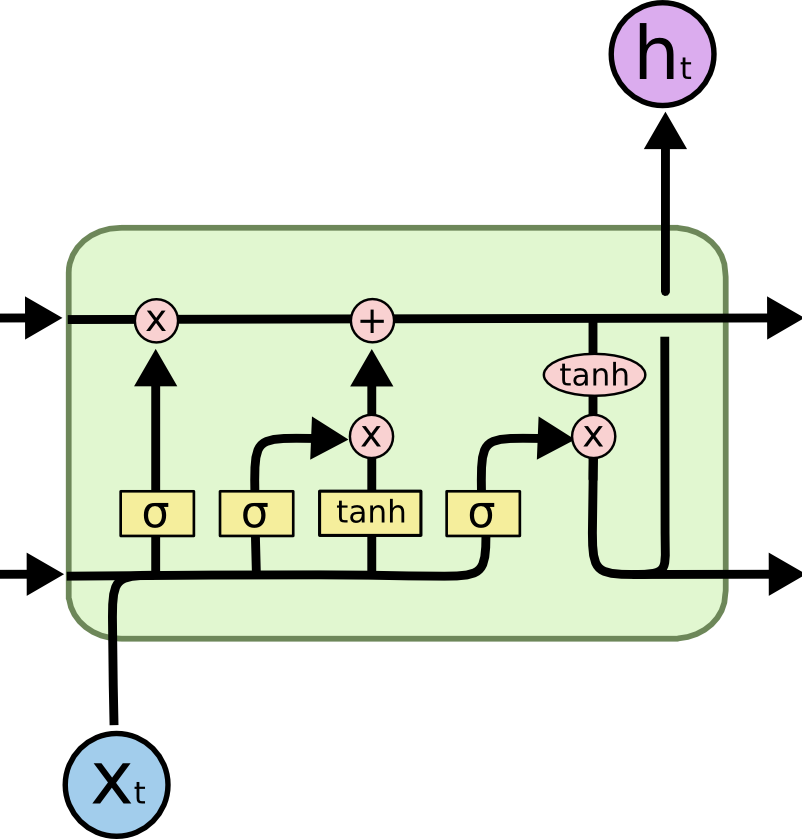
\includegraphics[scale=0.5]{figs/lstm_cell.png}
            \end{center}
            \caption{A single LSTM cell. From \cite{olah2015understanding}.}
            \label{fig:lstm_cell}
        \end{figure}

        As can be seen in the Figure \ref{fig:lstm_cell}, there are quite a few more parameters in this cell than in a normal RNN cell. 
        The calculation of the output vector and the hidden vector involves several operations.
        First of all the network determines how much of the hidden state to forget, also called the forget gate. 
        This is done by pushing both the previous iteration's output ($c_{t-1}$) and the forget gate vector ($f_t$) through a matrix multiplication, allowing the network to forget values at specific indices in the previous iteration's output vector. 
        $f_t$ can be obtained by using formula in Equation \eqref{eq:forget_vector_lstm}, where $W$ contains the weights for the input and $U$ contains the weights for the previous iteration's output vector, $x_t$ refers to the input, $h_{t-1}$ to the previous iteration's output vector and $b$ is bias:
        \begin{equation}
            f_t = \sigma(W_f x_t + U_f h_{t-1} + b_f)
            \label{eq:forget_vector_lstm}
        \end{equation}

        The network then determines what to remember from the input vector.
        This, commonly referred to as the input gate, is done by pushing the previous forget gate's output as well as the input gate through a matrix addition. 
        The output of the input gate ($i_t$) can be found by using the following formula:

        \begin{equation}
            i_t = \sigma(W_i x_t + U_i h_{t-1} + b_i)
            \label{eq:input_vector_lstm}
        \end{equation}

        The final hidden state vector ($c_t$) can then be found by using the previous two results as follows:

        \begin{equation}
            c_t = f_t \circ c_{t-1} + i_t \circ \sigma(W_c x_t + U_c h_{t-1} + b_c)
            \label{eq:hidden_state_vector_lstm}
        \end{equation}

        where $\circ$ denotes the Hadamard product (where each value at index $ij$ is the product of the values at the indices $ij$ in the two input matrices).
        This vector is then passed on to the next iteration. 
        Now the output gate vector $o_t$ and the output state $h_t$ can be optained:

        \begin{align} 
            o_t &= \sigma(W_o x_t + U_o h_{t-1} + b_o) \label{eq:output_gate_lstm}\\
            h_t &= o_t \circ \sigma(c_t) \label{eq:hidden_output_gate_lstm}
        \end{align}

        This results in a version of an RNN that is able to remember more and is more liberal in choosing what information it wants to keep in the hidden state and what it wants to discard. 
        This makes LSTM networks better suited for tasks involving series of data and become the predominant RNN architecture. 

        \paragraph{Gated Recurrent Units} Another RNN architecture is the GRU, introduced in \cite{cho2014learning}. 
        This architecture combines the input and forget gates into a single so-called ``update gate'' and also merges the cell state and hidden state (see Figure \ref{fig:gru_cell}). 
        The calculation of the merged output vector once again consists of several operations.
        The network first computes the ``reset gate'' $r_t$ using the following function, where $W_r$ are the weights for the reset gate and $[h_{t-1}, x_t]$ signifies the concatenation of $h_{t-1}$ and $x_t$:

        \begin{figure}[h!]
            \begin{center}
                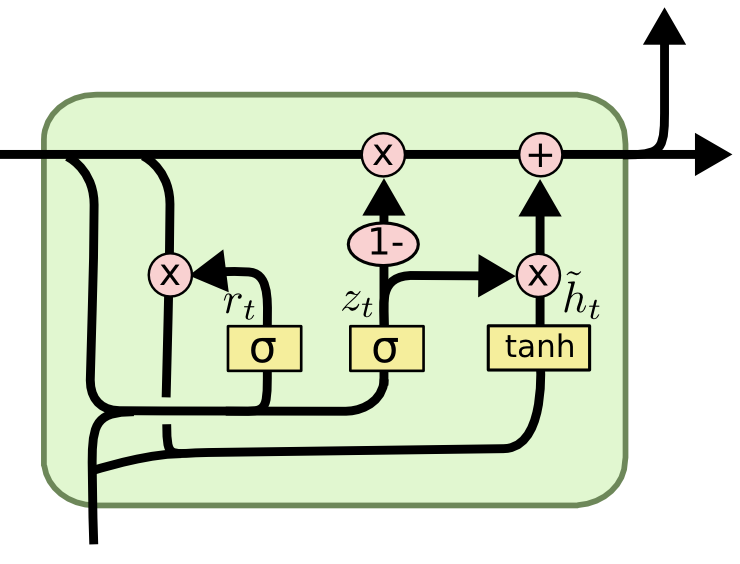
\includegraphics[scale=0.5]{figs/gru_cell.png}
            \end{center}
            \caption{A single GRU variation cell. From \cite{olah2015understanding}.}
            \label{fig:gru_cell}
        \end{figure}

        \begin{equation}
            r_t = \sigma\left(W_r [h_{t-1}, x_t]\right)
            \label{eq:gru_reset_gate}
        \end{equation}

        After this, the ``update gate'' $z_t$ is computed as follows, where $W_z$ holds the weights of the update gate:

        \begin{equation}
            z_t = \sigma\left(W_z [h_{t-1}, x_t]\right)
            \label{eq:gru_update_gate}
        \end{equation}

        The output vector $h_t$ (representing both the cell's output and its state) can then be computed by the following formula:

        \begin{equation}
            h_t = (1 - z_t) * h_{t-1} + z_t * \tilde{h_t}
            \label{eq:gru_output}
        \end{equation}

        where $\tilde{h_t} = \tanh(W * [r_t * h_{t-1}, x_t])$.

        % \paragraph{Bidirectional RNNs} It should be mentioned that when RNNs are used, they are often wrapped with a bidirectional layer.
        % This simply reverts the input sequence and enters the sequence in both the original and the reverse direction to two separate RNNs, usually LSTM or GRU.
        % % The usefulness of this is particularly intuitive when looking at the network in Figure \ref{fig:rnn}. 
        % When processing the entry $x^{(j)}$, only the entries $t < j$ are known. 
        % However, tokens later in the sequence might have an impact on the previous outputs of the model. 
        % Bidirectional RNNs are able to capture patterns that are overlooked by regular RNNs.

    %!TEX root = ../../main.tex

\subsection{Dimensionality Reduction Algorithms}
    Dimensionality reduction techniques are important in many applications related to machine learning.
    They aim to find low-dimensional embedding that should preserve sufficient information from the original dimension.
    Let's define $X = \{\boldsymbol{x}_{ik}|i=(1,..,c);k=(1,..,n_{i})\}$ as training samples where $\boldsymbol{x}_{ik} \in R^{d}$ is the $k^{th}$ sample of the $i^{th}$ class, $d$ is the original dimension of data, $m$ is the desired dimension of data after transformation such that $m < d$.

    \subsubsection{Linear discriminant analysis}
        The linear discriminant analysis (LDA) technique is developed to linearly transform the features into a lower dimensional space where the ratio of the between-class variance to the within-class variance is maximized, thereby guaranteering the optimal class separability.
        The projection results of $X$ on the lower dimensional space is denoted by $Y = \{\boldsymbol{y}_{ik} = w^T\boldsymbol{x}_{ik}|i=(1,..,c); k=(1,...,n_{i})\}$. $\boldsymbol{S}_B^y$ and $\boldsymbol{S}_W^y$ are computed as follows: 

        \begin{align}
            \boldsymbol{S}_W^y &= \sum_{i=1}^{c}\sum_{k=1}^{n_{i}}(y_{ik}-\boldsymbol{\mu}_i)(y_{ik}-\boldsymbol{\mu}_i)^T \label{eq:LDA_Sw_y}\\
            \boldsymbol{S}_B^y &= \sum_{i=1}^{c}n_i(\boldsymbol{\mu}_i - \boldsymbol{\mu})(\boldsymbol{\mu}_i - \boldsymbol{\mu})^T \label{eq:LDA_Sb_y}
        \end{align}

        where $\boldsymbol{\mu}_i=\frac{1}{n_i}{\sum_{k=1}^{n_{i}}}{\boldsymbol{y}_{ik}}$ is the mean of all samples of the $i^{th}$ class in the lower dimensional space; $\boldsymbol{\mu}=\frac{1}{n}\sum_{i=1}^{c}{\sum_{k=1}^{n_{i}}{\boldsymbol{y}_{ik}}}$ is the mean of all samples of all classes; $n=\sum_{i=1}^{c}n_i$ is the total number of data samples.
        The between-class $\boldsymbol{S}_B^y$ and within-class $\boldsymbol{S}_W^y$ covariance matrices in new dimension are not known yet but can be formulated as the linearly transformed versions of their counterparts $\boldsymbol{S}_B^x$ and $\boldsymbol{S}_W^x$ in original dimension.

        \begin{align}
            \boldsymbol{S}_W^y &= \omega^T\boldsymbol{S}_W^x\omega\\
            \boldsymbol{S}_B^y &= \omega^T\boldsymbol{S}_B^x\omega
        \end{align}

        $\boldsymbol{S}_B^x$ and $\boldsymbol{S}_W^x$ are easily calculable as follow:

        \begin{align}
            \boldsymbol{S}_W^x &= \sum_{i=1}^{c}\sum_{k=1}^{n_{i}}(x_{ik}-\boldsymbol{\mu}_i^{(x)})(x_{ik}-\boldsymbol{\mu}_i^{(x)})^T \label{eq:LDA_Sw_x}\\
            \boldsymbol{S}_B^x &= \sum_{i=1}^{c}n_i(\boldsymbol{\mu}_i^{(x)} - \boldsymbol{\mu}^{(x)})(\boldsymbol{\mu}_i^{(x)} - \boldsymbol{\mu}^{(x)})^T \label{eq:LDA_Sb_x}
        \end{align}

        Then the objective function is formulated by a Rayleigh quotient:

        \begin{equation}
            \boldsymbol{\omega}^* = \operatorname*{argmax}_{\boldsymbol{\omega}}\frac{trace(\boldsymbol{S}_B^y)}{trace(\boldsymbol{S}_W^y)} = \operatorname*{argmax}_{\boldsymbol{\omega}}\frac{trace(\omega^T\boldsymbol{S}_B^x\omega)}{trace(\omega^T\boldsymbol{S}_W^x\omega)}
            \label{eq:LDA}
        \end{equation}

        The Fisher's criterion in Equation \eqref{eq:LDA} can be reformulated as:

        \begin{equation}
            \boldsymbol{S}_W^x\omega = \lambda\boldsymbol{S}_B^x\omega
        \end{equation}

        where $\lambda$ represents the eigenvalues of the transformation matrix $\omega$. The analytical solution of $\boldsymbol{\omega}^*$ is optained by calculating the eigenvectors $V = \{v_1,v_2,...,v_m\}$ sorted by the scalar values of corresponding eigenvalues $\lambda = \{\lambda_1,\lambda_2,...,\lambda_m\}$ of the matrix $\boldsymbol{S} = {\boldsymbol{S}_W^x}^{-1}\boldsymbol{S}_B^x$.

    \subsubsection{Pairwise-covariance linear discriminant analysis}
        Pairwise-covariance linear discriminant analysis (pc-LDA) is an extension of LDA introduced in \cite{kong2014pairwise} that overcomes it's drawbacks by formulating pairwise distances between pairs of classes.
        The pairs of $a$ and $b$ classes are regarded as two Gaussian distributions $\mathcal{N}_a(\mu_a,{\boldsymbol{S}_W^y}_a), \mathcal{N}_b(\mu_b,{\boldsymbol{S}_W^y}_b)$ and the objective distance between two classes is defined as their Kullback-Leibler divergence \cite{kullback1951}:

        \begin{equation}
            D_{KL}\left(\mathcal{N}_a\parallel\mathcal{N}_b\right)=\frac{1}{2}\left(\mu_a-\mu_b\right)^{T}{\left({\boldsymbol{S}_W^y}_{ab}\right)}^{-1}\left(\mu_a-\mu_b\right),
        \end{equation}

        where ${\boldsymbol{S}_W^y}_{ab}$ is pairwise covariance matrix (Equation \eqref{eq:pc-LDA_Sw_ab}), calculated as the $\beta$ parameterized convex sum of global within-class scatter matrix $\boldsymbol{S}_W^y$ used in LDA with the within-class scatter matrix of each class ${\boldsymbol{S}_W^y}_i$ (Equation \eqref{eq:pc-LDA_Sw_i}).
        The author theorizes it would better represent the data distribution within two classes.

        \begin{align}
            {\boldsymbol{S}_W^y}_i &= \sum_{j=1}^{v}\sum_{k=1}^{n_{ij}}{\left(y_{ik}-\mu_i\right)\left(y_{ik}-\mu_i\right)^T} \label{eq:pc-LDA_Sw_i}\\
            {\boldsymbol{S}_W^y}_{ab} &= \beta\frac{n_a{\boldsymbol{S}_W^y}_a+n_b{\boldsymbol{S}_W^y}_b}{n_a+n_b}+\left(1-\beta\right){\boldsymbol{S}_W^y}
            \label{eq:pc-LDA_Sw_ab}
        \end{align}

        where $n_a$ and $n_b$ are number of samples belonging to class $a$ and $b$. The final objective is properly weighted to focus on classes with more samples:

        \begin{equation}
            \operatorname*{min}_{\boldsymbol{\omega}}{J}=\sum_{a=1}^{c}\sum_{b=a+1}^{c}{\frac{n_an_b}{{[2D_{KL}\left(\mathcal{N}_a\parallel\mathcal{N}_b\right)]}^q}},\ \ s.t.\ \omega^T\omega=\boldsymbol{I}
            \label{eq:pc-LDA}
        \end{equation}

        here $q\ge1$ is a hyper-parameter that controls how much the pairs of classes with smaller objective distances are biased over the others.

        The new model of pc-LDA is solved with a variant of gradient descent described in \cite{kong2014pairwise}, where $\nabla J\left(\omega\right)$ is computed and $\omega$ is updated as Equation \eqref{eq:pc-LDA_omega} in order to enforce $\omega$ on the Stiefel manifold. Every several iterations, due to numerical error, the learnt transformation is unitarized $\omega \leftarrow \omega{\left(\omega^T\omega\right)}^{-\frac{1}{2}}$ to ensure that the constraint $\omega^T\omega = \boldsymbol{I}$ is satisfied.

        \begin{equation}
            \omega \leftarrow \omega - \eta\left(\nabla J - \omega{[\nabla J]}^T\omega\right)
            \label{eq:pc-LDA_omega}
        \end{equation}

    %!TEX root = ../../../main.tex

\subsection{Multi-view Learning Algorithms}

    The motivation of multi-view learning (MvL) algorithms is to construct a common low-dimensional embedding that should preserve sufficient information or even be more informative than each individual view.

    Let's define $X = \{\boldsymbol{x}_{ijk}|i=(1,..,c);j = (1,..,v);k=(1,..,n_{ij})\}$ as samples from $v$ views where $\boldsymbol{x}_{ijk} \in R^{d_j}$ is the $k^{th}$ sample from the $j^{th}$ view of the $i^{th}$ class, $d_j$ is the dimensions of data at the $j^{th}$ view.
    Here ${\boldsymbol x}_{ijk}$ is a feature vector extracted from the $k^{th}$ sample from the $j^{th}$ view of the $i^{th}$ class.
    Different methods for features extraction from single view have been presented in previous sections. 

    \subsubsection{Multi-view discriminant analysis}
        Multi-view discriminant analysis (MvDA) is an extension of LDA for multi-view scenario \cite{kan2015multi}.
        It tries to determine a set of $v$ linear transformations to project all action samples from each view $j = (1,..,v)$ to a common space.
        The projection results of $X$ on the common space is denoted by $Y = \{\boldsymbol{y}_{ijk} = w_j^T\boldsymbol{x}_{ijk}|i=(1,..,c); j=(1,..,v); k=(1,...,n_{ij})\}$.
        The common space is built by maximizing the between-class variation $\boldsymbol{S}_B^y$ while minimizing the within-class variation $\boldsymbol{S}_W^y$ from all views. $\boldsymbol{S}_B^y$ and $\boldsymbol{S}_W^y$ are computed as follows: 

        \begin{align}
            \boldsymbol{S}_W^y &= \sum_{i=1}^{c}\sum_{j=1}^{v}\sum_{k=1}^{n_{ij}}(y_{ijk}-\boldsymbol{\mu}_i)(y_{ijk}-\boldsymbol{\mu}_i)^T \label{eq:MvDA_Sw}\\
            \boldsymbol{S}_B^y &= \sum_{i=1}^{c}n_i(\boldsymbol{\mu}_i - \boldsymbol{\mu})(\boldsymbol{\mu}_i - \boldsymbol{\mu})^T \label{eq:MvDA_Sb}
        \end{align}

        where $\boldsymbol{\mu}_i=\frac{1}{n_i}\sum_{j=1}^{v}{\sum_{k=1}^{n_{ij}}}{\boldsymbol{y}_{ijk}}$ is the mean of all samples of the $i^{th}$ class from all views in the common space; $\boldsymbol{\mu}=\frac{1}{n}\sum_{i=1}^{c}\sum_{j=1}^{v}{\sum_{k=1}^{n_{ij}}{\boldsymbol{y}_{ijk}}}$ is the mean of all samples of all classes from all views in the common space; $n=\sum_{i=1}^{c}n_i$ is the total data samples from all views.

        In order to separate the unknown transformation vectors, the between-class and within-class scatter matrices are reformulated as:

        \begin{align}
            \boldsymbol{S}_W^y &= W^{T}X\left(\boldsymbol{I} - \boldsymbol{E}\right)X^{T}W\\
            \boldsymbol{S}_B^y &= W^{T}X\left(\boldsymbol{E} - \frac{1}{n}\boldsymbol{\mathbbm{1}}\right)X^{T}W
        \end{align}
        where $W = \{\omega_1,\omega_2,...,\omega_v\}$ is concatenation of transformation vectors of all views; $\boldsymbol{I} \in \mathbb{R}^{n\times n}$ is identity matrix; $\boldsymbol{\mathbbm{1}} \in \mathbb{R}^{n\times n}$ is matrix of ones; $\boldsymbol{E} \in \mathbb{R}^{n\times n}$ is a square matrix whose elements satisfy:
        \begin{equation}
            \boldsymbol{E}_{kl} = \left\{\begin{array}{lr}
                \frac{1}{n_i}, & \text{if } class(x_k) = class(x_l) = i\\
                0, & \text{otherwise}
                \end{array}\right\}
        \end{equation}

        Then the objective function is formulated by a Rayleigh quotient:

        \begin{align}
            (\boldsymbol{\omega}_1^*,\boldsymbol{\omega}_2^*, ..., \boldsymbol{\omega}_v^*) &= \operatorname*{argmax}_{\boldsymbol{\omega}_1, \boldsymbol{\omega}_2,..., \boldsymbol{\omega}_v}\frac{trace({S}_B^y)}{trace({S}_W^y)}\\
            \boldsymbol{W}^* &= \operatorname*{argmax}_{\boldsymbol{W}}\frac{trace(W^{T}[X\left(\boldsymbol{E} - \frac{1}{n}\boldsymbol{\mathbbm{1}}\right)X^{T}]W)}{trace(W^{T}[X\left(\boldsymbol{I} - \boldsymbol{E}\right)X^{T}]W)}
            \label{eq:MvDA}
        \end{align}

        According to \cite{kan2016multi}, the problem satisfies the optimization form of generalized eigenvalue problem and could be analytically solved through eigenvalue decomposition.
        The concatenated $\boldsymbol{W}^* = \{\boldsymbol{\omega}_1^*,\boldsymbol{\omega}_2^*, ..., \boldsymbol{\omega}_v^*\}$ could be computed using the same procedure as $\boldsymbol{\omega}^*$ in LDA.
        Similarly, MvDA can be used as a dimensionality reduction algorithm by choosing $m$ eigenvectors corresponding to $m$ leading eigenvalues.

    \subsubsection{Multi-view discriminant analysis with view-consistency}

        In \cite{kan2016multi}, the authors observed that as multiple views correspond to the same objects, there should be some correspondence between multiple views.
        They then introduce a view consistency constraint into the objective function, that means if $X_j, X_r$ are observed at $j^{th}$ and $r^{th}$ views, there exists a certain transformation $\boldsymbol{R}$ such that $X_j = \boldsymbol{R}X_r$.
        As a result, the transformations obtained from two views (i.e. the projection of features extracted from singe view to common view) should have similar relationship: ${\omega}_j = \boldsymbol{R}{\omega}_r$.
        Let's define $\beta_i$ that captures the structure of the transformation ${\omega}_i$.

        \begin{equation}
            \omega_i = X_i\boldsymbol\beta_i
            \label{eq:MvDA-vc_beta}
        \end{equation}

        Then the $\beta_j$ and $\beta_r$ capturing the structures of two transformations of two views $j$ and $r$ should be identical ${\beta}_j = {\beta}_r$.

        Generalizing to $v$ views, suppose that ${\boldsymbol\beta}_j, j=(1,..,v)$ captures the structures of $v$ transformations ${w}_j$.
        Following the above observation, the $\boldsymbol{\beta}_r, r=(1,..,v)$ should resemble mutually.
        That means the similarity between the pair of $\boldsymbol{\beta}_j$ and $\boldsymbol{\beta}_r$ should be minimized. 

        \begin{equation}
            \sum_{j,r=1}^{v}||\boldsymbol{\beta_j} - \boldsymbol{\beta_r}||_2^2
            \label{eq:MvDA-vc_vc}
        \end{equation}

        From Equation \eqref{eq:MvDA-vc_beta}, we have:

        \begin{equation}
            \boldsymbol\beta_i = {\left(X_i^{T}X_i\right)}^{-1}X_i^{T}\omega_i \triangleq \boldsymbol{P}_iw_i
        \end{equation}

        Replacing in Equation \eqref{eq:MvDA-vc_vc} we can reformulate it as:

        \begin{equation}
            \sum_{j,r=1}^{v}||\boldsymbol{\beta_j} - \boldsymbol{\beta_r}||_2^2 = trace\left(W^{T}\boldsymbol{P}^{T}\left(2((v - 1)\boldsymbol{I} - \boldsymbol{\mathbbm{1}})\right)\boldsymbol{P}W\right)
        \end{equation}
        where $\boldsymbol{P} = \{\boldsymbol{P}_1,\boldsymbol{P}_2,...,\boldsymbol{P}_v\}$; $\boldsymbol{I} \in \mathbb{R}^{n\times n}$ is identity matrix; $\boldsymbol{\mathbbm{1}} \in \mathbb{R}^{n\times n}$ is matrix of ones.
        This term is called in \cite{kan2016multi} {\itshape view consistency} and will be added to the denominator of Equation \eqref{eq:MvDA}

        \begin{align}
            (\boldsymbol{\omega}_1^*,\boldsymbol{\omega}_2^*, ..., \boldsymbol{\omega}_v^*) &= \operatorname*{argmax}_{\boldsymbol{\omega}_1, \boldsymbol{\omega}_2,..., \boldsymbol{\omega}_v}\frac{trace({S}_B^y)}{trace({S}_W^y) + \alpha\sum_{j,r=1}^{v}||\boldsymbol{\beta_j} - \boldsymbol{\beta_r}||_2^2}\\
            \boldsymbol{W}^* &= \operatorname*{argmax}_{\boldsymbol{W}}\frac{trace(W^{T}[X\left(\boldsymbol{E} - \frac{1}{n}\boldsymbol{\mathbbm{1}}\right)X^{T}]W)}{trace(W^{T}[X\left(\boldsymbol{I} - \boldsymbol{E}\right)X^{T} + 2\alpha\boldsymbol{P}^T\left((v - 1)\boldsymbol{I} - \boldsymbol{\mathbbm{1}}\right)\boldsymbol{P}]W)}
            \label{eq:MvDA-vc}
        \end{align}

        This optimization problem could also be analytically solved by relaxing to the trace ratio optimization problem as Equation \eqref{eq:MvDA}.
        In the Equation \eqref{eq:MvDA-vc}, $\alpha$ is an empirically chosen parameter that puts a weight on the view-consistency assumption.
        When $\alpha = 0$, the MvDA-vc becomes the original MvDA. 


    %!TEX root = ../../main.tex

\section{Related Works} \label{sec:related_works}

    \subsection{Human action and gesture recognition}
        Action recognition has been an attractive research topic since the last decade \cite{zhang2019comprehensive}.
        Early methods represented human actions by extracting 2D/3D key-points such as Harris-3D, SIFT-3D, HOG-3DHOF \cite{laptev2008learning}, ESURF \cite{willems2008efficient} then computed a descriptor from the detected key-points.
        Action representation  by a set of key-points could loose the temporal information. Therefore, Wang and Schmid in \cite{wang2013action} proposed a feature named improved dense trajectories (iDT) that densely sample and track optical flow points along trajectories.
        iDT has become state-of-the-art hand-crafted features and widely used for many video-based tasks.
        However, when working with large-scale datasets, iDT becomes intractable on due to its expensive computational cost and poor performance. 

        To work with more challenging datasets, effective action recognition approaches rely on powerful learning methods, particularly the deep learning techniques.
        Early works applied 2D CNN on frames of video sequence and then aggregated the information using pooling techniques \cite{karpathy2014large}.
        To exploit the temporal information, different architectures such as LSTM with the internal mechanisms called gates that can deal with short-term memory are proposed \cite{sun2017lattice}.
        Recently, instead of using 2D convolutional operators, different 3D CNN have been proposed \cite{ji20123d, tran2015learning, varol2017long}.
        Besides, to boost the recognition performance, different approaches tried to combine multiple streams \cite{wang2015towards, feichtenhofer2016convolutional, khong2018improving} or to combine both multiple features \cite{wang2015action, christoph2016spatiotemporal}. %trajectory-pooled deep-convolutional
        %descriptor - TDD;  ST-ResNet+iDT
        %Recently, many other architectures such as temporal Segment Networks - TSN \cite{wang2016temporal}, ST-VLMPF \cite{duta2017spatio}, P3D ResNet \cite{qiu2017learning}, I3D\cite{carreira2017quo}, 3D ResNeXt \cite{hara2018can}, R(2+1) D-TwoStream \cite{tran2018closer}, CO2FI+ASYN \cite{lin2018action}, and DML \cite{chen2017deep} have shown state-of-the-art performances in action recognition.
        %Previous section briefly gives a survey of different techniques for features extraction and action recognition from common views.

        These aforementioned approaches focus on single view action recognition, cross-view action recognition is more challenging and requires additional techniques to be taken into account. 
        Junejo et al. in \cite{junejo2008cross} proposed a descriptor, namely self-similarity matrix (SSM), which is an exhaustive table of distances between image features taken by pair from the image sequences.
        Liu et al. \cite{liu2011cross} employed cuboids extracted from each video and BoW model to build video descriptor for each single view. Then, a bipartite graph is built to model two view-dependent vocabularies.
        Li et al. \cite{li2012discriminative} described each video by concatenating spatio-temporal interest-point-based descriptor with shape flow descriptor. Then, to deal with cross-view, they construct ‘virtual views’, each is a linear transformation between action descriptors from one viewpoint and those from another.
        The method in \cite{zheng2012cross, zheng2013learning} employed the same video representation manner as in \cite{li2012discriminative}.
        However, a transferable dictionary between source and target view has been learnt to force features of the same action extracted from two views having the same sparse representation. 
        %In \cite{ulhaq2017space}, the authors proposed an advanced space-time filtering framework for recognizing human actions despite large viewpoint variations. Specifically, they used 3D tensor structure at each pixel, which characterizes the most common local motion in action sequences. Discrete tensor Fourier transform is then applied to achieve frequency domain representations. Then, they form view clusters from multiple-view action data and use space-time correlation filtering to achieve robust view representations. 

        Previous cross-view action recognition techniques usually connect source and target views with a set of linear transformations, that are unable to capture the non-linear manifolds on which real actions lie. In \cite{rahmani2017learning}, the authors find a shared high-level non-linear virtual path that connects multiple source and target views to the same canonical view. This virtual path is learnt by a deep neural network. In \cite{kong2017deeply}, a deep learning technique that stacks multiple layers of feature learners is designed to incorporate both private and shared view features. 
        In \cite{liu2018hierarchically}, the authors concatenated both private and shared view features and learnt transferable dictionary pair from a pair of views. In \cite{zhang2018action}, the authors proposed a framework to jointly learn a a view-invariant transfer dictionary and a view-invariant classifier using synthetic data during the pre-training phase to extract view-invariance between 3D and 2D videos.

        %As we have analyzed, multi-view  analysis has been actively studied. Several innovative ideas have been proposed. As a result, performance of multi-view classification is significantly improved. However, most of these methods are experimented on still images. The question of how still good those methods a special time-series data (i.e. video data) has been not addressed. In this paper, we contribute to improve the model of common feature space. In addition, we will evaluate the proposed method on video data, where both temporal and spatial features must be taken into account.

    \subsection{Multi-view analysis and learning techniques}
        As many objects in the real-world can be observed from different viewpoints, to exploit the consensual and complementary information between different views, Multi-view analysis (MvA) techniques are employed.
        MvA is a strategy for fusing data from different sources or subsets.

        Canonical Correlation Analysis (CCA) \cite{Hotelling} can be considered as the first approach of MvL with the aim to find pairs of projections for two views so that the correlations between these views are maximized.
        As CCA can only handle the linear correlation, Kernel CCA (KCCA) was proposed to take non-linear correlation relationship of data into account \cite{Akaho2006}.
        However, both CCA and KCCA are unsupervised methods and can not leverage the label information.
        In \cite{diethe2008multiview}, a supervised approach named Multi-view Fisher discriminant analysis (MvFDA) was proposed for binary classification problem.
        All of aforementioned methods are only applicable for two views problem.

        To extend to multiple view cases, a natural extension is to maximize the sum of the pairwise correlations.
        In a general case, it would be better to build a common shared feature space that captures latent information of the object from all observed views.
        For this propose, Multi-view CCA (MvCCA) is proposed in 2010 to build a common feature space of all views \cite{rupnik2010multi}. 
        %MCCA tried to find $v$ transformations by maximizing the correlation of every two views. 
        However, MvCCA did not consider the discrepancy information but only maximizing the correlation between every two views, so that it may be ineffective for classification across views. 
        %Generalized Multi-view Analysis (GMA) preserves the supervised structure of each view while keeping the projections of different views close to each other in the latent common space. GMA is considered as an extension of Fisher Discriminant analysis (FDA) for cross-view problem. It considers class label information so it could be good for multi-view classification. However, GMA considers only the the discriminant information in each individual view, not inter-view so it could decrease cross-view recognition.
        %Multi-view Uncorrelated Linear Discriminant Analysis (MULDA) \cite{sun2015multi-view} learnt uncorrelated discriminant features by using Uncorrelated Linear Discriminant Analysis (ULDA). Multi-view Modular Discriminant Analysis (MvMDA) \cite{cao2017generalized} was proposed to separate class centers across different views. 

        In \cite{kan2015multi}, Multi-view discriminant analysis (MvDA), an extension of linear discriminant analysis (LDA) for multi-view problem was proposed.
        MvDA tries to optimize jointly view correlation, intra-view and inter-view discriminability. 
        An extension of MvDA which considers view-consistency was also introduced and achieved significant performance improvement.

        In \cite{zhao2018multi}, the authors proposed multi-view manifold learning with locality alignment (MvML-LA) framework to realize manifold learning under multi-view scenario. 
        %Locality alignment in the latent space learning is considered to enhance its discriminative capability and developed two specific algorithms in supervised and unsupervised scenarios, respectively. 

        Most recently, \cite{you2019multi} proposed Multi-view Common Component Discriminant Analysis (MvCCDA) technique that both integrates supervised information and local geometric information into the common component extraction process.
        This helps to effectively handle view discrepancy, discriminability and non-linearity in a joint manner.


    \section{Summary}
        In this chapter, various related works were briefed.
        The general concepts of deep neural networks, especially 3D CNN because of its outstanding performance in action recognition for video data, are explained.
        Also, the underlying mathematical model behind LDA and two utilized multi-view analysis algorithms inspired by it (MvDA \& MvDA-vc) were clarified.
        In addition, an extension of LDA called pc-LDA that enhances it with better class discrepancy constraints were introduced.

    %!TEX root = ../../main.tex

\chapter{Proposed method} \label{chap:method}
    \section{Introduction}
        This chapter represents the methodology proposed in this thesis.
        Section \ref{sec:general_framework} gives an overview of the multi-view human action and gesture recognition framework.
        Section \ref{sec:feature_extraction} provides the details on different CNN architectures used in feature extraction for individual view.
        Section \ref{sec:common_feature_space} describes the proposed improvement of MvDA for building common feature space across multiple views.

    %!TEX root = ../../main.tex

\section{General Framework} \label{sec:general_framework}
    We propose a framework for cross-view action recognition as illustrated in Figure \ref{fig:frw}. It composes of two phases: training phase and recognition phase. 
    \begin{itemize}
        \item \textbf{Training phase}: Suppose we have $v$ views. The training phase consists of three main steps: 
        \begin{enumerate}
            \item \textit{Feature extraction at separated view}: All training samples from each separated view will be passed though a feature extraction step. Different deep techniques will be investigated, including 2D CNNs based feature extraction combined with aggregation techniques and 3D CNNs based feature extraction, to output the final descriptor for each video sample. Let's call the features extracted at this step as features at single views or separated view features. 
            \item \textit{Common space construction}: This step builds a common feature space so that samples belonging to the same class will be close to each other even they are captured from different viewpoints. It takes all separated view features extracted from training set from the previous step and find a set of $v$ linear transformations $({\omega}_1, {\omega}_2, ..., {\omega}_v)$ that minimize within-class variation while maximizing between-class variation of features in the projected space (common space). 
            \item \textit{Training classifier}: Once $v$ transformations have been computed, the projected features in the common space of each view will be utilized to train a simple predictive model $F$ (i.e. kNN).
        \end{enumerate}
        \item \textbf{Recognition phase}. Multi-view recognition consists of two following steps:
        \begin{enumerate}
            \item \textit{Feature extraction} Features of the testing sample $x_j$ from the view $V_j$ are extracted. This feature will be projected in the pre-built common space by the corresponding transformation ${\omega}_j$. The projected feature is denoted as $y_j = {\omega}^T_j*x_j$.
            \item \textit{Class prediction}: The projected feature $y_j$ will be passed into the classifier $F(y_j)$ that outputs the label of action.
        \end{enumerate}
    \end{itemize}

    \begin{figure}[htbp]
        \centering
        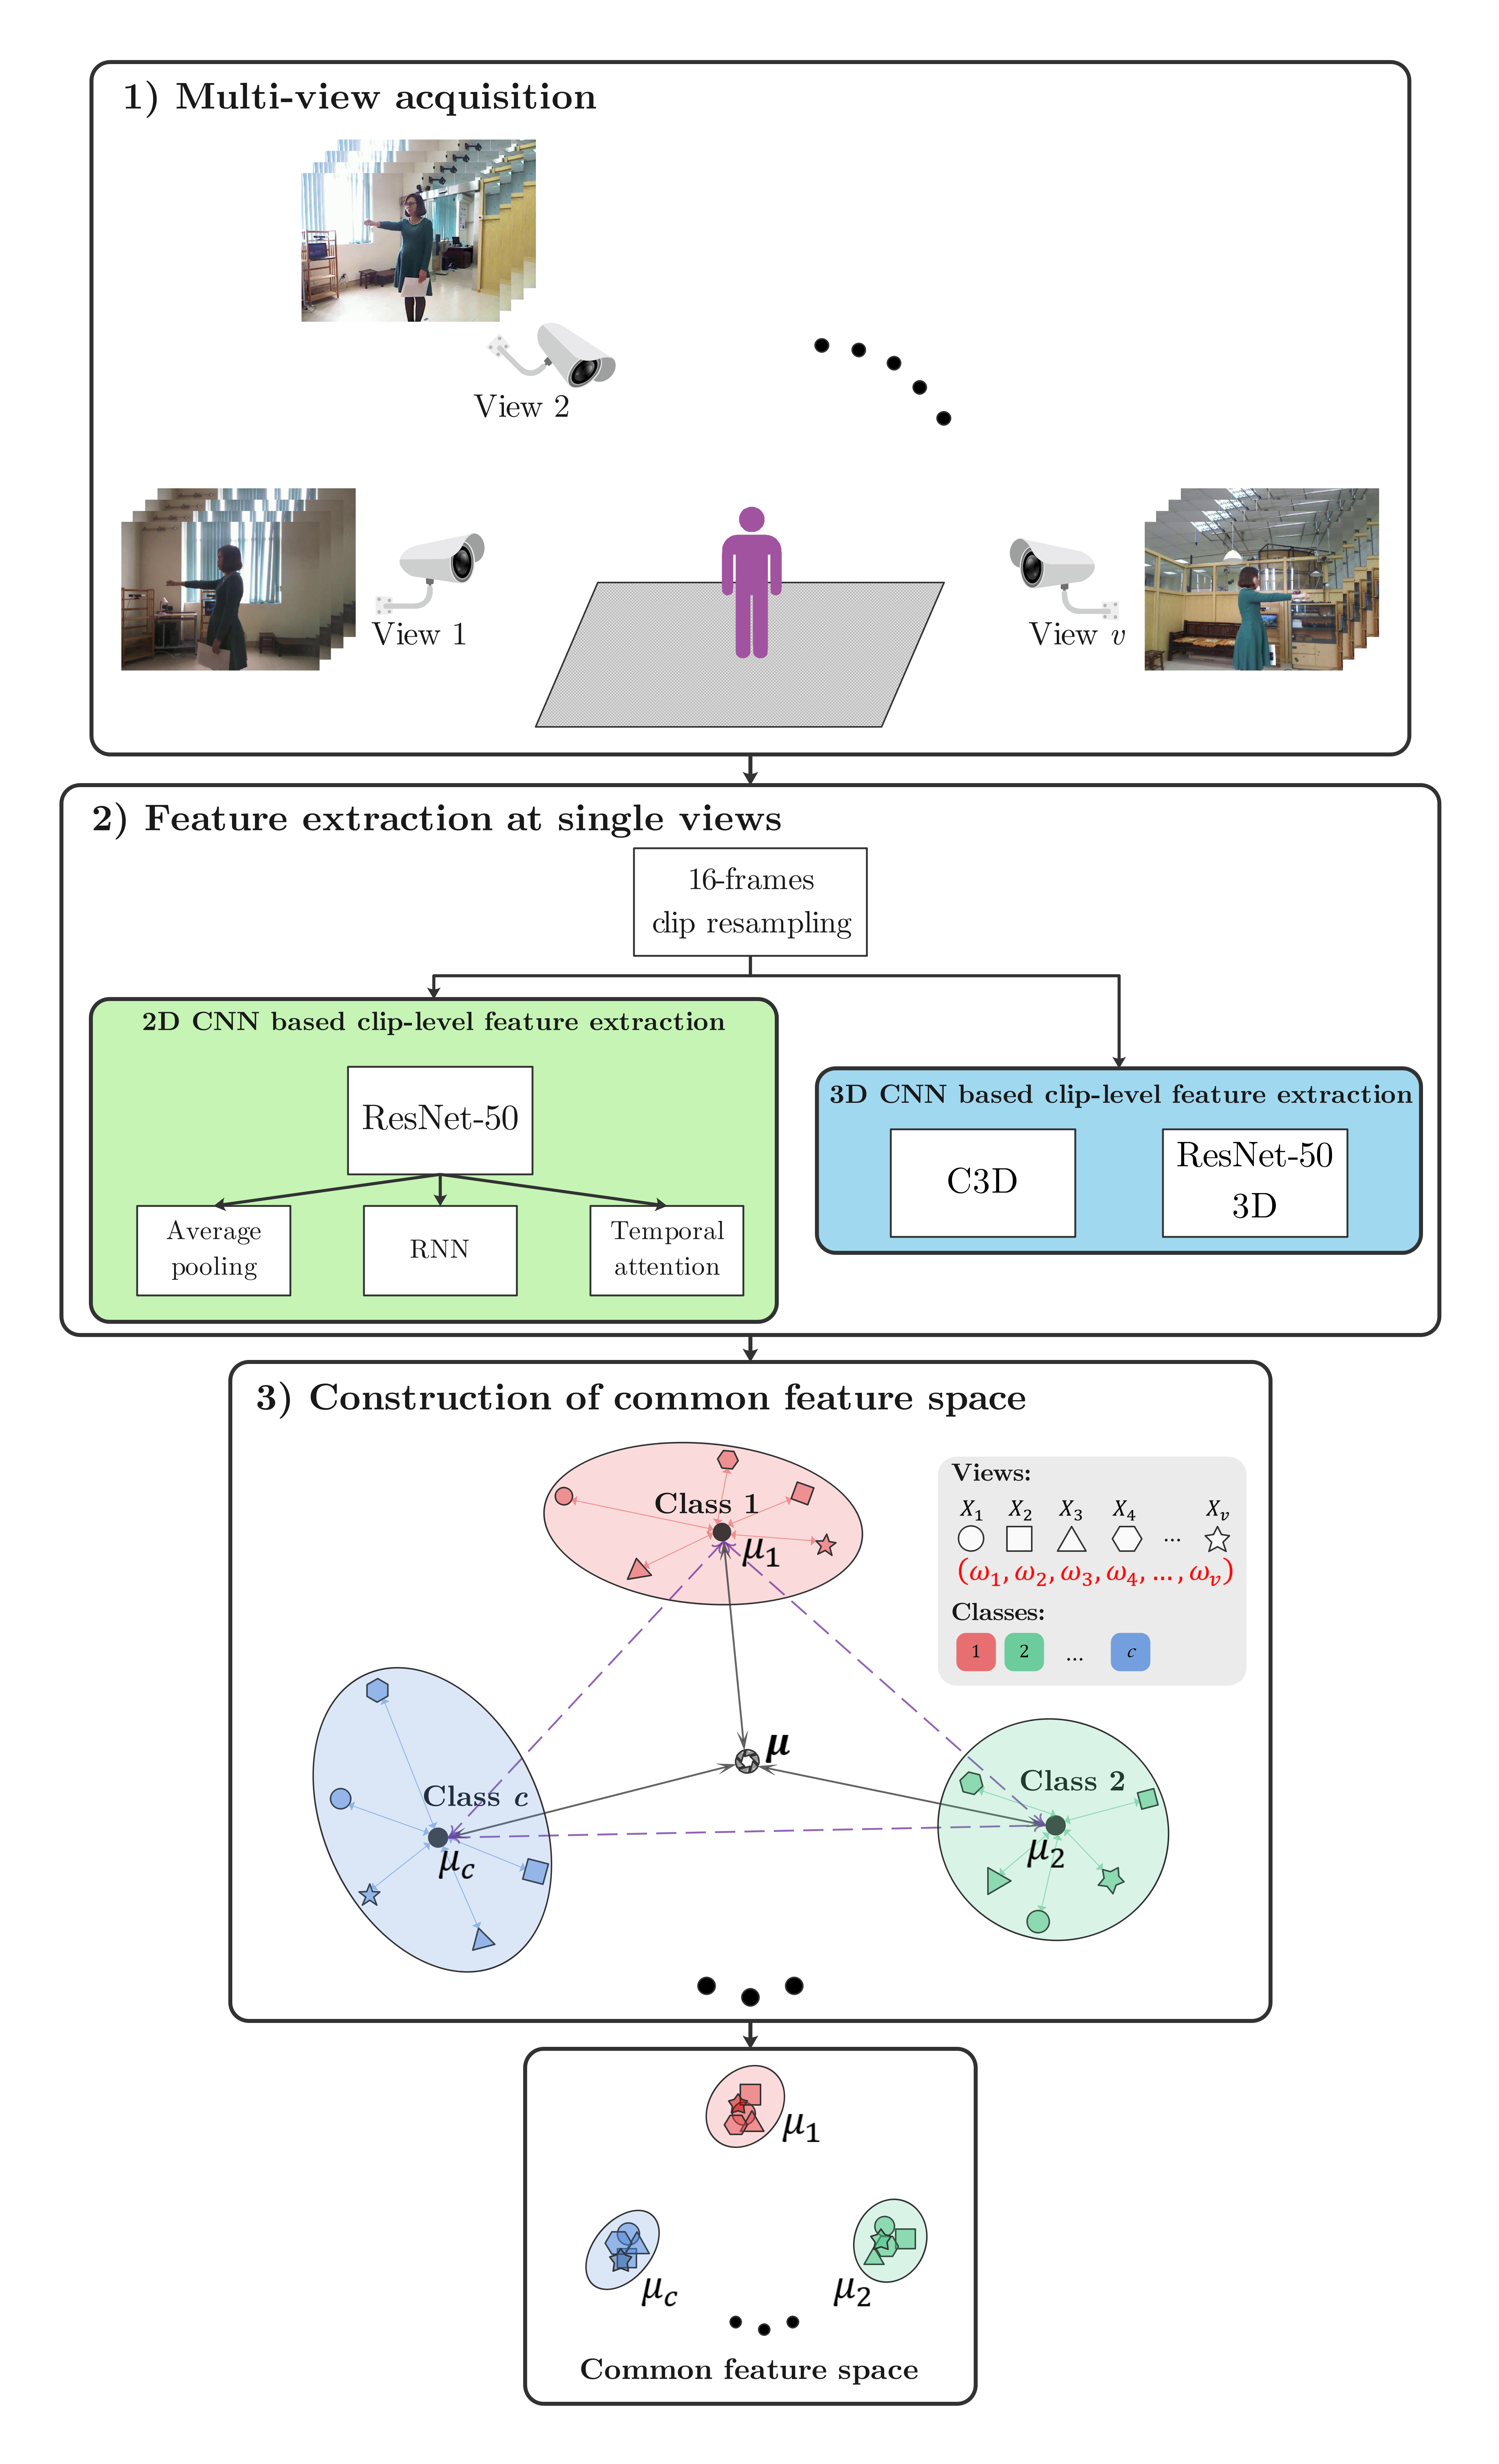
\includegraphics[width=0.85\linewidth]{figs/Framework.png}
        \caption{Proposed framework for building common feature space with pairwise-covariance multi-view discriminant analysis (pc-MvDA).}
        %\vspace{-0.3cm}
        \label{fig:frw}
    \end{figure}
    %In the following, I will detail the step of feature extraction at separated view in subsection \ref{sub:private}, the step of building the common feature space in subsection \ref{sub:common}. 

    %!TEX root = ../../../main.tex

\section{Feature extraction at individual view using deep learning techniques} \label{sec:private}
    %!TEX root = ../../../main.tex

\subsection{2D CNN based clip-level feature extraction}
    First, the ResNet-50 Convolution Neural Network \cite{he2016deep} is used as a 2D CNN network to extract spatial features of each frame in video. Fig.\ref{fig:resnet50} illustrates the architecture of ResNet-50 which composes of five convolutional blocks stacked on top of each other. The network is pre-trained on ImageNet then fine-tuned using training sets described in Section \ref{sec:experimentalresult}. Deep residual features are extracted from the output of the last convolutional block of the network which is a 2048-D feature vector. 
    \begin{figure}[htbp]
        \centering
        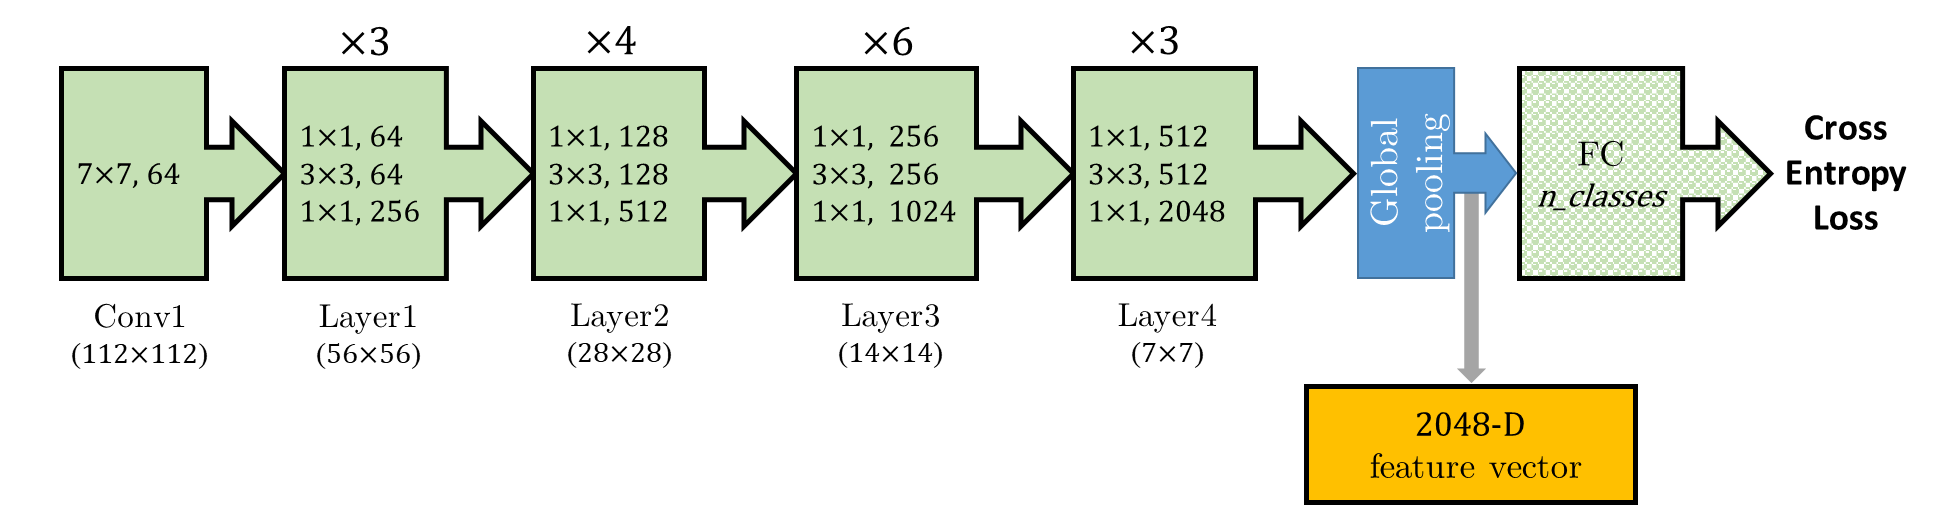
\includegraphics[width=1\linewidth]{Figs/Resnet50.png}
        \caption{Architecture of ResNet-50 utilized in our work for feature extraction at each separated view}
        %\vspace{-0.3cm}
        \label{fig:resnet50}
    \end{figure}
    We then aggregate frame-level features to create video-level features. In this work, we implement three temporal modeling techniques: 1) average pooling (AP); 2) recurrent neural network (RNN) and 3) temporal attention (TA). Fig.\ref{fig:pooling} illustrates three techniques.
    \begin{figure}[htbp]
        \centering
        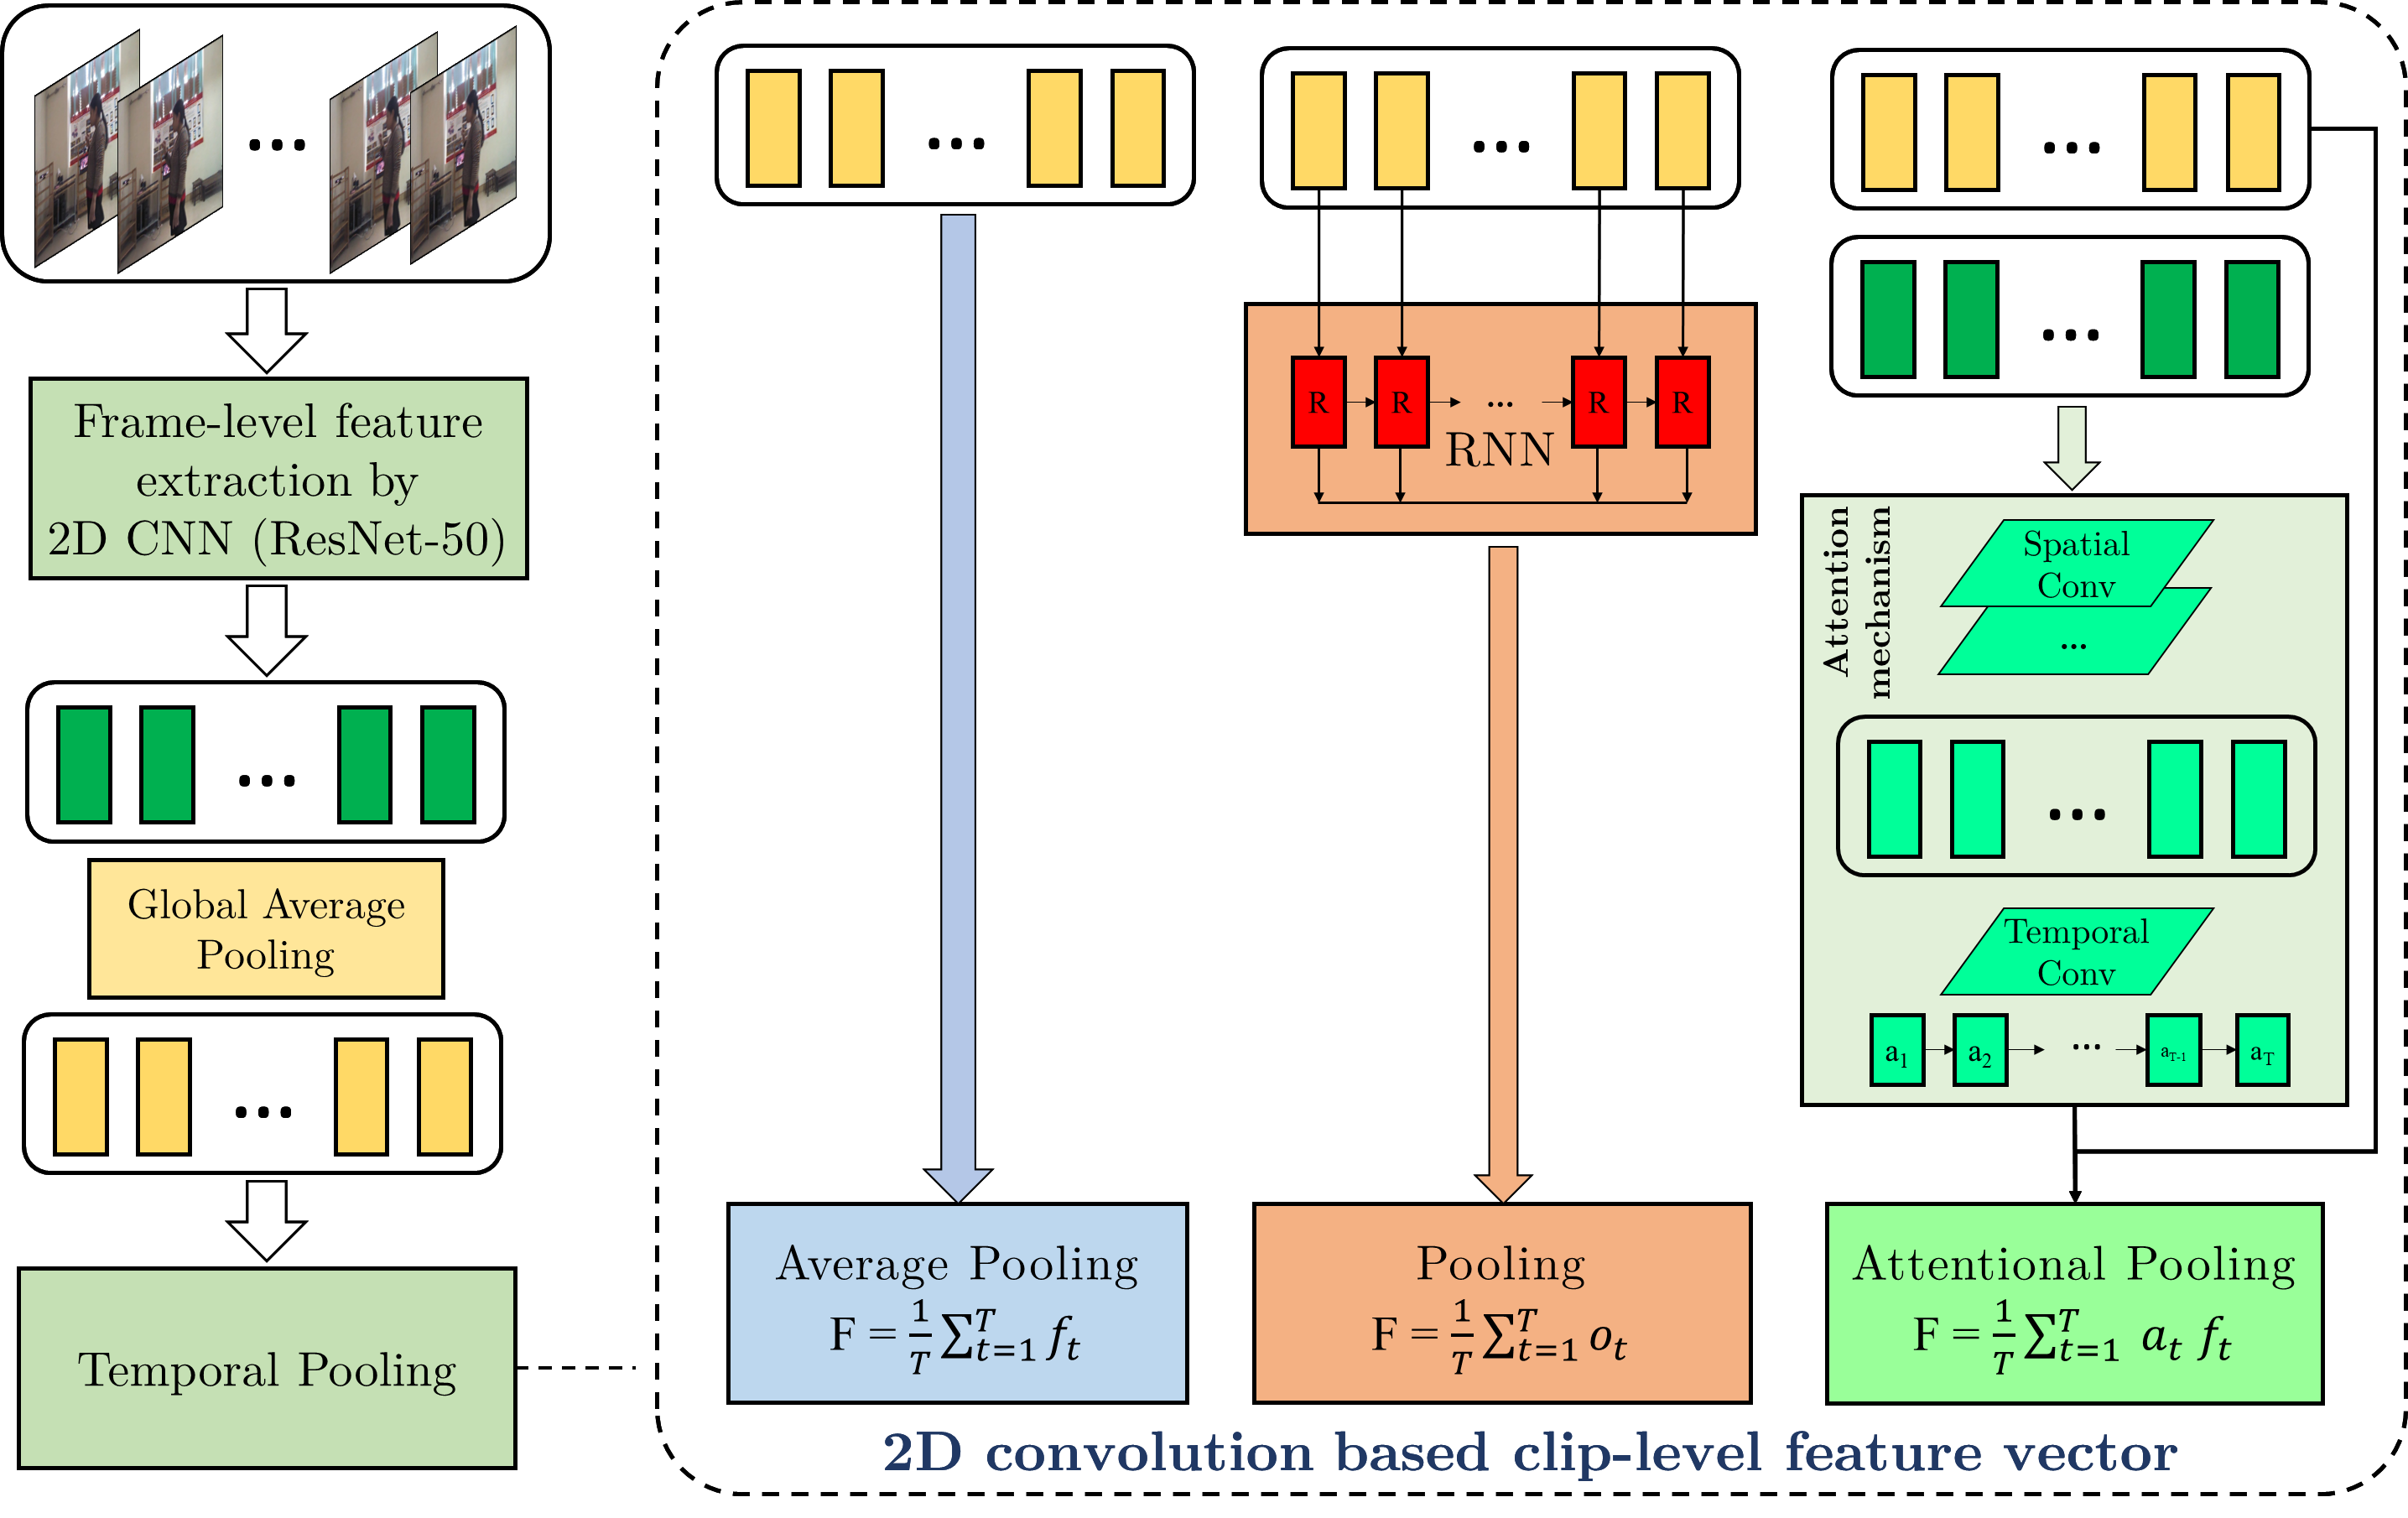
\includegraphics[width=1\linewidth]{Figs/Pooling.png}
        \caption{Three pooling techniques: Average Pooling (AP), Recurrent Neural Network (RNN) and Temporal Attention Pooling (TA)}
        %\vspace{-0.3cm}
        \label{fig:pooling}
    \end{figure}

    \textbf{Average Pooling - AP}: Let ${f}$ be the video-level feature, ${f_t}$ be the frame-level feature at time ${t}$, $T$ be the number of frames in video. Average pooling technique simply averages all frame-level features uniformly to create the video-level feature:
    \begin{equation}
    f=\frac{1}{T}\sum_{t=1}^T{f_t}
    \end{equation}
    As a frame-level feature is a 2048-D vector, the video-level feature is of the same dimension.\\
    \textbf{Recurrent Neural Network - RNN}: An RNN cell encodes a $t^{th}$ frame-level feature at time $t$ of the sequence and passes the hidden state $h_t$ into the next time step. In our work, a cell is a LSTM (Long Short Term Memory). The RNN is a single-layer with $T$ cells. Each cell outputs a 512-D feature vector that contains information of the current frame and the previous ones. We aggregate a sequence of frame-level features into a video-level feature $f$ by calculating the average of the RNN outputs $o_t = R(f_t, o_{t-1})$;$t \in [1;T]$. 
    \begin{equation}
    f=\frac{1}{T}\sum_{t=1}^T{o_t}
    \end{equation}
    \textbf{Temporal Attention - TA}: In the above pooling techniques, frame-level features are equally aggregated. In reality, some frames may have more important roles than remaining ones in recognizing an action. In temporal attention model, we learn a weight $a_t$ for each frame $f_t$ and apply an attention weighted average on the sequence of frame-level features as follows.
    \begin{equation}
    f=\frac{1}{T} \sum_{t=1}^{T}a_{t}f_{t}
    \end{equation}
    To learn the weights $a_t, t \in [1,T]$, we adopt the attention generation network proposed by Jiyang Gao et al. \cite{gao2018revisiting}. The network takes a sequence of frame-level features $[T, w, h, 2048]$, each is tensor extracted from the last convolution layer of ResNet-50. The network architecture consists of two main components: Spatial Convolution and Temporal Convolution. First, a conv layer with shape $\{w,h,2048,d_t\}$ is applied, then we get a $d_t$-dimensional feature for each frame of the clip ($d_t$ = input channel). Then we apply a temporal conv layer $\{3,d_t, 1\}$ on these frame-level features to generate temporal attentions $s_c^t$. Once we have $s_c^t$, the final attention score $a_t$ is computed by Softmax function: 
    \begin{equation}
    a_t = \frac{e^{s_c^t}}{\sum_{k=1}^{T}e^{s_c^k}}
    \end{equation}
    %In all scenarios of pooling, we train the whole net (including a ResNet-50 combined with RNN, TA or AP) on our training set according to the evaluation protocols presented in section \ref{sec:experimentalresult}.

    %!TEX root = ../../../main.tex

\subsection{3D CNN based clip-level feature extraction}
    3D convolution network architectures is increasingly concerned with video based problems. 
    %The main idea of 3D CNN is to utilize 3D convolution operators $(x,y,t)$ instead of 2D operators $(x, y)$, where $x, y$ are spatial dimensions and $t$ is temporal dimension. As a result, 3D CNNs can directly extract video-level features that contain both spatial and temporal information. 
    In this thesis, two 3D CNN architectures are deployed: C3D \cite{duta2017spatio} and ResNet-50 3D \cite{hara2018can}. 

    \textbf{ResNet 3D}: ResNet-50 3D adopts 3D convolution kernels with ResNet-50 architecture. %We apply transfer learning by using Kinetics pre-trained weights \cite{kay2017kinetics}. Like most of the methods presented above, we also get a 2048-dimensional feature vector for each video with input tensor shape $[3, 16, 224, 224]$. They are the number of channels per image (c), the number of frames in the video (s), the width (w) and the height (h) of the frame respectively. 
    The architecture of ResNet-50 3D network is described in the Figure \ref{fig:resnet50_3d}. It has similar architecture as the ResNet-50 but the convolution layers uses 3D operation.  
    \begin{figure}[htbp]
        \centering
        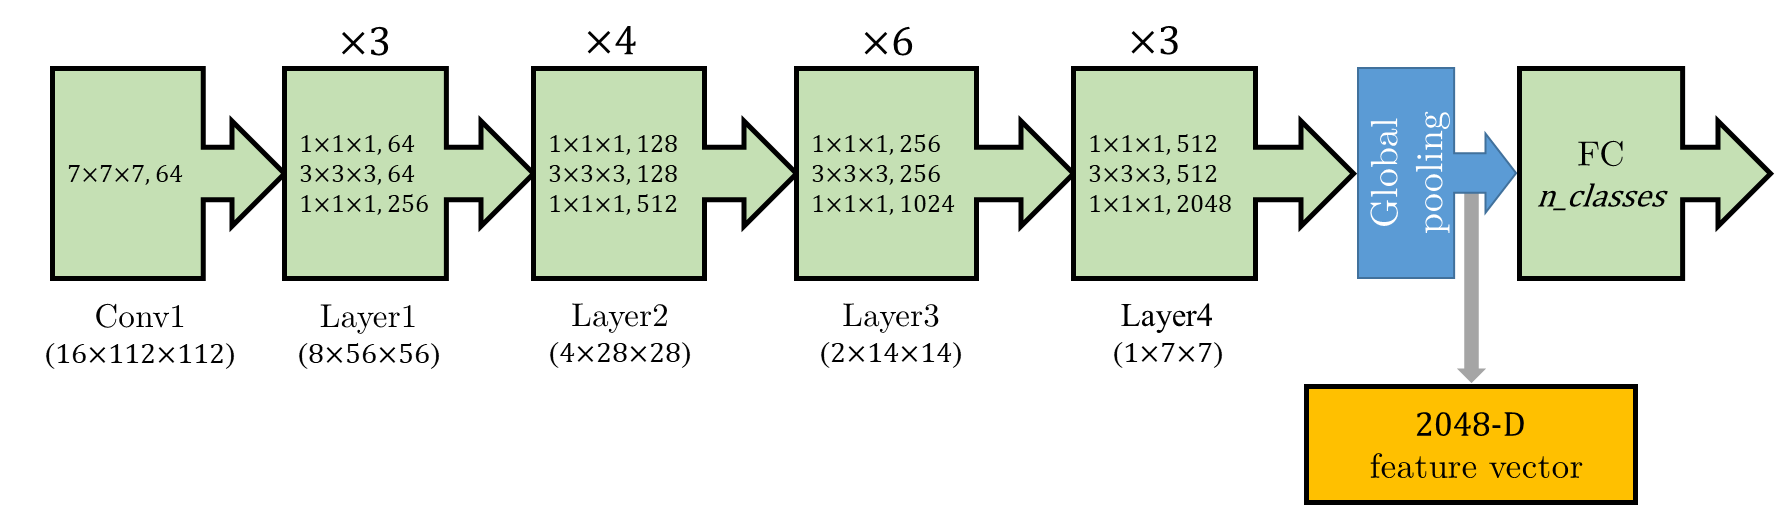
\includegraphics[width=1\linewidth]{Figs/Resnet50_3D.png}
        \caption{Architecture of ResNet-50 3D utilized in this work for feature extraction}
        %\vspace{-0.3cm}
        \label{fig:resnet50_3d}
    \end{figure}

    \textbf{C3D}: 3D deep convolution neural network, which was introduced in \cite{tran2015learning}, has shown to be very efficient for action recognition tasks. C3D takes input as an image sequence instead of a static image, computes the 3D convolution on each 3D cubes from video clip. By doing so, C3D captures both spatial and temporal characteristics of action at the same time.
    \begin{figure}[htbp]
        \centering
        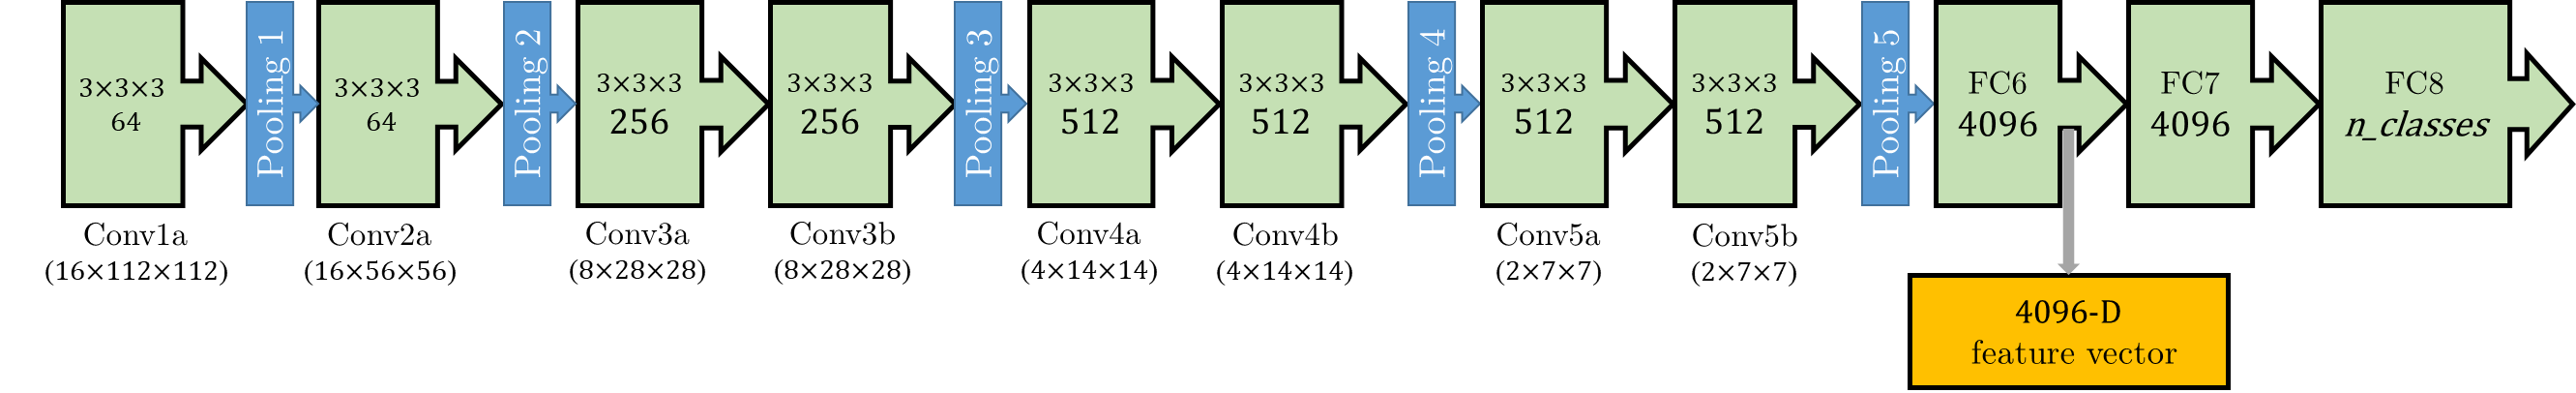
\includegraphics[width=1\linewidth]{Figs/C3D.png}
        \caption{Architecture of C3D utilized in this work for feature extraction}
        %\vspace{-0.3cm}
        \label{fig:C3D}
    \end{figure}
    A C3D network contains 8 convolution, 5 max-pooling and 2 fully connected layers as illustrated in Figure \ref{fig:C3D}. 
    % The number of filters of convolution layers from Conv1 to Conv5 are 64, 128, 256, 512, 512 respectively. All 3D convolution kernels are of size $3\times3\times3$ with stride $1\times1\times1$ and followed by a 3D batch normalization layer. 
    % We utilize the network pre-trained on Sports-1M and fine-tuned on Kinetics dataset.
    The feature vector of 4096 dimensions extracted from FC\-6 layer will be served for training and testing classifiers in further steps.

    To apply in the proposed framework of action and gestures recognition, transfer learning technique is applied for pretrained models on each data stream corresponding to each individual view.
    Details of pre-trained weights and training process of the networks will be presented in Section \ref{sec:experimental_setup}.


    %!TEX root = ../../../main.tex

\section{Construction of common feature space} \label{sec:common}
    %!TEX root = ../../../main.tex

\subsection{Brief summary of Multi-view Discriminant Analysis}
    Suppose that actions belonging to $c$ classes are observed from $v$ views, the number of samples from the $j^{th}$ view of the $i^{th}$ class is $n_{ij}$. We define $X = \{\boldsymbol{x}_{ijk}|i=(1,..,c);j = (1,..,v);k=(1,..,n_{ij})\}$ as samples from $v$ views where 
    $\boldsymbol{x}_{ijk} \in R^{d_j}$ is the $k^{th}$ sample from the $j^{th}$ view of the $i^{th}$ class, $d_j$ is the dimensions of data at the $j^{th}$ view. Here ${\boldsymbol x}_{ijk}$ is a feature vector extracted from the $k^{th}$ sample from the $j^{th}$ view of the $i^{th}$ class. Different methods for features extraction from single view have been presented in previous sections. 

    \textbf{Multi-view discriminant analysis (MvDA)}
    MvDA was an extension of LDA for multi-view scenario \cite{kan2015multi}. It tries to determine a set of $v$ linear transformations to project all action samples from each view $j = (1,..,v)$ to a common space. The projection results of $X$ on the common space is denoted by $Y = \{\boldsymbol{y}_{ijk} = w_j^T\boldsymbol{x}_{ijk}|i=(1,..,c); j=(1,..,v); k=(1,...,n_{ij})\}$. The common space is built by maximizing the between-class variation $\boldsymbol{S}_B^y$ while minimizing the within-class variation $\boldsymbol{S}_W^y$ from all views. $\boldsymbol{S}_B^y$ and $\boldsymbol{S}_W^y$ are computed as follows: 
    \begin{align}
        \boldsymbol{S}_W^y &= \sum_{i=1}^{c}\sum_{j=1}^{v}\sum_{k=1}^{n_{ij}}(y_{ijk}-\boldsymbol{\mu}_i)(y_{ijk}-\boldsymbol{\mu}_i)^T \label{eq:MvDA_Sw}\\
        \boldsymbol{S}_B^y &= \sum_{i=1}^{c}n_i(\boldsymbol{\mu}_i - \boldsymbol{\mu})(\boldsymbol{\mu}_i - \boldsymbol{\mu})^T \label{eq:MvDA_Sb}
    \end{align}
    where $\boldsymbol{\mu}_i=\frac{1}{n_i}\sum_{j=1}^{v}{\sum_{k=1}^{n_{ij}}}{\boldsymbol{y}_{ijk}}$ is the mean of all samples of the $i^{th}$ class from all views in the common space; $\boldsymbol{\mu}=\frac{1}{n}\sum_{i=1}^{c}\sum_{j=1}^{v}{\sum_{k=1}^{n_{ij}}{\boldsymbol{y}_{ijk}}}$ is the mean of all samples of all classes from all views in the common space; $n=\sum_{i=1}^{c}n_i$ is the total data samples from all views.
    Then the objective function is formulated by a Rayleigh quotient:
    \begin{equation}
        (\boldsymbol{\omega}_1^*,\boldsymbol{\omega}_2^*, ..., \boldsymbol{\omega}_v^*) = \operatorname*{argmax}_{\boldsymbol{\omega}_1, \boldsymbol{\omega}_2,..., \boldsymbol{\omega}_v}\frac{trace({S}_B^y)}{trace({S}_W^y)}
        \label{eq:MvDA}
    \end{equation}
    According to \cite{kan2016multi}, the optimization problem could be analytically solved through generalized eigenvalue decomposition. 

    %\textbf{Multi-view discriminant analysis with view consistency (MvDA-vc):}
     In \cite{kan2016multi}, the authors observed that as multiple views correspond to the same objects, there should be some correspondence between multiple views. They then introduce a view consistency constraint into the objective function. The method is called as MvDA-vc. In this paper, we will also compare with MvDA-vc but our method improves the MvDA, so we will not detail MvDA-vc in this section. 
     
     %According to the experimental results presented in the next section, MvDA-vc helps to improves significantly performance of recognition. However, it is difficult to explain explicitly and intuitively how view consitency helpts
     
    %  , that means if $\boldsymbol{X}_j, \boldsymbol{X}_r$ are observed at $j^{th}$ and $r^{th}$ views, then there exists a certain transformation $\boldsymbol{R}$ such that $\boldsymbol{X}_j = \boldsymbol{R}\boldsymbol{X}_r$. As a result, the transformations obtained from two views (i.e. the projection of features extracted from singe view to common view) should have similar relationship: ${\omega}_j = \boldsymbol{R}{\omega}_r$. Let us define $\beta_i$ that captures the structure of the transformation ${\omega}_i$. Then the $\beta_j$ and $\beta_r$ capturing the structures of two transformations of two views $j$ and $r$ should be identical ${\beta}_j = {\beta}_r$.
     
    %  Generalizing to $v$ views, suppose that ${\boldsymbol\beta}_j, j=(1,..,v)$ captures the structures of $v$ transformations ${w}_j$. Following the above observation, the $\boldsymbol{\beta}_r, r=(1,..,v)$ should resemble mutually. That means the similarity between the pair of $\boldsymbol{\beta}_j$ and $\boldsymbol{\beta}_r$ should be minimized. 
    % \begin{equation}
    %      \sum_{j,r=1}^{v}||\boldsymbol{\beta_j} - \boldsymbol{\beta_r}||_2^2
    % \end{equation}
    %  This term is called in \cite{kan2016multi} {\itshape view consistency} and will be added to the denominator of Eq.\eqref{eq:MvDA}
    % \begin{equation}
    % \small
    %     (\boldsymbol{\omega}_1^*,\boldsymbol{\omega}_2^*, ..., \boldsymbol{\omega}_v^*) = \operatorname*{argmax}_{\boldsymbol{\omega}_1, \boldsymbol{\omega}_2,..., \boldsymbol{\omega}_v}\frac{trace({S}_B^y)}{trace({S}_W^y) + \alpha\sum_{j,r=1}^{v}||\boldsymbol{\beta_j} - \boldsymbol{\beta_r}||_2^2} 
    %     \label{eq:MvDA-vc}
    % \end{equation}
    % Similarly, this optimization problem could be analytically solved by relaxing to the ratio trace problem as Eq.\eqref{eq:MvDA}. In the Eq.\eqref{eq:MvDA-vc}, $\alpha$ is an empirically chosen parameter. It puts a weight on the view-consistency assumption. When $\alpha = 0$, the MvDA-vc becomes the original MvDA. 

    %!TEX root = ../../../main.tex

\subsection{Pairwise-covariance Multi-view Discriminant Analysis pc-MvDA}
    MvDA emphasizes on finding a common space with minimal within-class variation while the distances between class means and global mean are jointly maximized. However, the distances between some pairs of classes can be disregarded. In this paper, to obtain this property, we modified MvDA with reformulated between and with-in class scatter matrices terms in a pairwise manner. First, let us define a new inter-class scatter matrix formula that takes paired distance into account:
    \begin{equation}
        \boldsymbol{S}_B^y=\sum_{a=1}^{c}\sum_{b=a+1}^{c}{\left(\mu_a-\mu_b\right)\left(\mu_a-\mu_b\right)^T}
    \end{equation}
    where $a$, $b$ are two distinct classes. For each pairs of class $a$ and class $b$, the between covariance is calculated as:
    \begin{equation}
        {\boldsymbol{S}_B^y}_{ab}={\left(\mu_a-\mu_b\right)\left(\mu_a-\mu_b\right)^T}
        \label{eq:Sb_ab}
    \end{equation}

    The intra-class scatter matrix $\boldsymbol{S}_W^y$ of MvDA is calculated as simple summation of all covariance matrices of each $i^{th}$ class, $i = {1,...,c}$:
    \begin{equation}
        {\boldsymbol{S}_W^y}_i=\sum_{j=1}^{v}\sum_{k=1}^{n_{ij}}{\left(y_{ijk}-\mu_i\right)\left(y_{ijk}-\mu_i\right)^T}
    \end{equation}

    Mathematically, it assumes data samples from each class among all views are identically Gaussian distributed, and contribute evenly to the minimization of intra-class scatter. In reality, it is hardly the case as data variations of samples from different classes and different view points are usually drastically diverse and may also have different dimensions.

    To better represent the distribution of data, pc-MvDA uses a paired intra-scatter matrix which is denoted as
    \begin{equation}
        {\boldsymbol{S}_W^y}_{ab}=\beta\frac{n_a{\boldsymbol{S}_W^y}_a+n_b{\boldsymbol{S}_W^y}_b}{n_a+n_b}+\left(1-\beta\right){\boldsymbol{S}_W^y}
        \label{eq:Sw_ab}
    \end{equation}
    where $0\le\beta\le1$ is a hyper-parameter for regularization between the original global intra-covariance ${\boldsymbol{S}_W^y}$ and the novel two local class covariances ${\boldsymbol{S}_W^y}_a$ and ${\boldsymbol{S}_W^y}_b$. This formulation is closer to the value of covariances of both classes than the standard intra-covariance.

    Instead of solving the vanilla generalized eigen value problem for the whole dataset, we split it into sub-problems for each pairs of class $a$ and $b$, in which we define the objective distance to be minimized between two corresponding classes.
    \textbf{Difference of our proposed method compared to pairwise LDA (pc-LDA)}
    In pc-LDA \cite{kong2014pairwise}, the pairs of $a$ and $b$ classes are regarded as two Gaussian distributions $\mathcal{N}_a(\mu_a,{\boldsymbol{S}_W^y}_a), \mathcal{N}_b(\mu_b,{\boldsymbol{S}_W^y}_b)$ and the objective distance between two classes is defined as their Kullback-Leibler divergence \cite{kullback1951}:
    \begin{equation}
        D_{KL}\left(\mathcal{N}_a\parallel\mathcal{N}_b\right)=\frac{1}{2}\left(\mu_a-\mu_b\right)^{T}{\left({\boldsymbol{S}_W^y}_{ab}\right)}^{-1}\left(\mu_a-\mu_b\right),
    \end{equation}
    Then the final objective is properly weighted to focus on classes with more samples:
    \begin{equation}
        \operatorname*{min}_{\boldsymbol{\omega}_1, \boldsymbol{\omega}_2,...,
        \boldsymbol{\omega}_v}{J}=\sum_{a=1}^{c}\sum_{b=a+1}^{c}{\frac{n_an_b}{{[2D_{KL}\left(\mathcal{N}_a\parallel\mathcal{N}_b\right)]}^q}}
        \label{eq:pc-LDA}
    \end{equation}
    here $q\ge1$ is a hyper-parameter that controls how much the pairs of classes with smaller objective distances are biased over the others.

    In our observation, the minimization of KL divergence for each pairs of classes $a$ and $b$ can be substituted by a generalized eigenvalue problem with the pairwise ${\boldsymbol{S}_W^y}_{ab}$ and the ${\boldsymbol{S}_B^y}_{ab}$ we defined. Although these sub-problems do not have an unified analytical solution to be solved concurrently, the criteria can be formulated in various differentiable ways like in \cite{fukunaga1990441} so we can use gradient descent algorithm:
    \begin{equation}
        J_1=\frac{tr(S_B)}{tr(S_W)};\quad 
        J_2=tr\left(\frac{S_B}{S_W}\right);\quad
        J_3=tr\left|\left|\frac{S_B}{S_W}\right|\right|;\quad
        J_4=\frac{det(S_B)}{det(S_W)}
    \end{equation}

    We choosed the former Fisher loss as the ratio of scalar values is computationally cheaper. Comparing to the objective of pc-LDA in Eq.\eqref{eq:pc-LDA}, our proposed model is obviously more efficient since it contains only simple operators and the need to inverse a singular-prone matrix is negated. Therefore, it is better fit in the scenario where we want to train the model multiple iterations over multi-view high dimensional output.

    Our final objective function of pairwise-covariance multi-view discriminant analysis is sum of all pairwise Fisher criteria with normalized weights:
    \begin{equation}
        \operatorname*{min}_{\boldsymbol{\omega}_1, \boldsymbol{\omega}_2,..., \boldsymbol{\omega}_v}{J}=\sum_{a=1}^{c}\sum_{b=a+1}^{c}{\frac{n_an_b}{n_{cc}^2}{\left[{\frac{trace\left({\boldsymbol{S}_W^y}_{ab}\right)}{trace\left({\boldsymbol{S}_B^y}_{ab}\right)}}\right]}^{q}}
        \label{eq:pc-MvDA}
    \end{equation}
    where $n_{cc}$ is the number of common components as coined in \cite{you2019multi} or simply number of samples in each view. This added normalization term assures that the objective does not depend on size of dataset.

    Let's look at the Fig.\ref{fig:frw}, the nominator of MvDA(-vc) $\boldsymbol{S}_B^y$ is the sum of all distances from mean of every class $\mu_i$, $i = {1,...,c}$ to the mean of all classes $\mu$. This helps to push class far away from the mean of all classes (the dotted green lines in Fig.\ref{fig:frw}). However, it may not ensure that the classes will be far from each other (Fig.\ref{fig:pc-MvDA}a). In this work, we take the pairwise distance into account and integrate them in an multi-view framework (the dotted violet lines in Fig.\ref{fig:frw}). Thanks to this, the classes will be more discriminated (Fig. \ref{fig:pc-MvDA}b). The algorithm for solving pc-MvDA is presented in supplemental materials. 

    \textbf{Illustrative examples:} We illustrate the advantage of pc-MvDA on artificial datasets. Firstly, using function provided by scikit-learn library, we generate several isotropic Gaussian blobs equal to desired number of classes as data samples from one single view. To generate other views, we clone and apply translation, point-wise noise and rotation with random orthogonal group multiplication to the first view.

    In Fig.\ref{fig:synthetic1}, MvDA and pc-MvDA results on 2D synthetic dataset of 180 data points in 2-D space. There are three classes, observed at three viewpoints. We show data distribution and 1-D projection results using MvDA and pc-MvDA respectively. We notice that data points of two classes (the first and the third classes) are close together in original space. When we project in common space by MvDA, these classes are still close together. In contrast, these classes are more discriminant when projected by pc-MvDA.

    Similar to the first example, in the second example, we generate 300 data points of 5 classes observed from 3 different views (Fig.\ref{fig:synthetic2}). We observe that the five clusters of pc-MvDa common space contract strongly and become more separated as compared to the MvDA results (especially the first and the fourth classes).

    \begin{figure}[htbp]
        \centering
        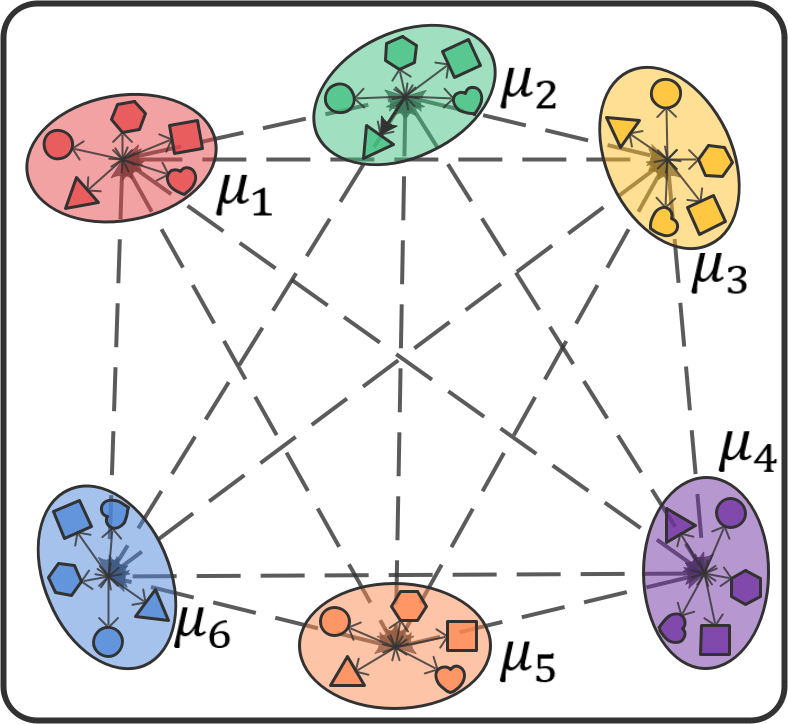
\includegraphics[width=0.7\linewidth]{Figs/pc-MvDA.png}
        \caption{a) MvDA does not optimize the distance between paired classes in common space. b) pc-MvDA takes pairwise distances into account then distinguish better the classes.}
        %\vspace{-0.3cm}
        \label{fig:pc-MvDA}
    \end{figure}

    \begin{figure}[htbp]
        \centering
        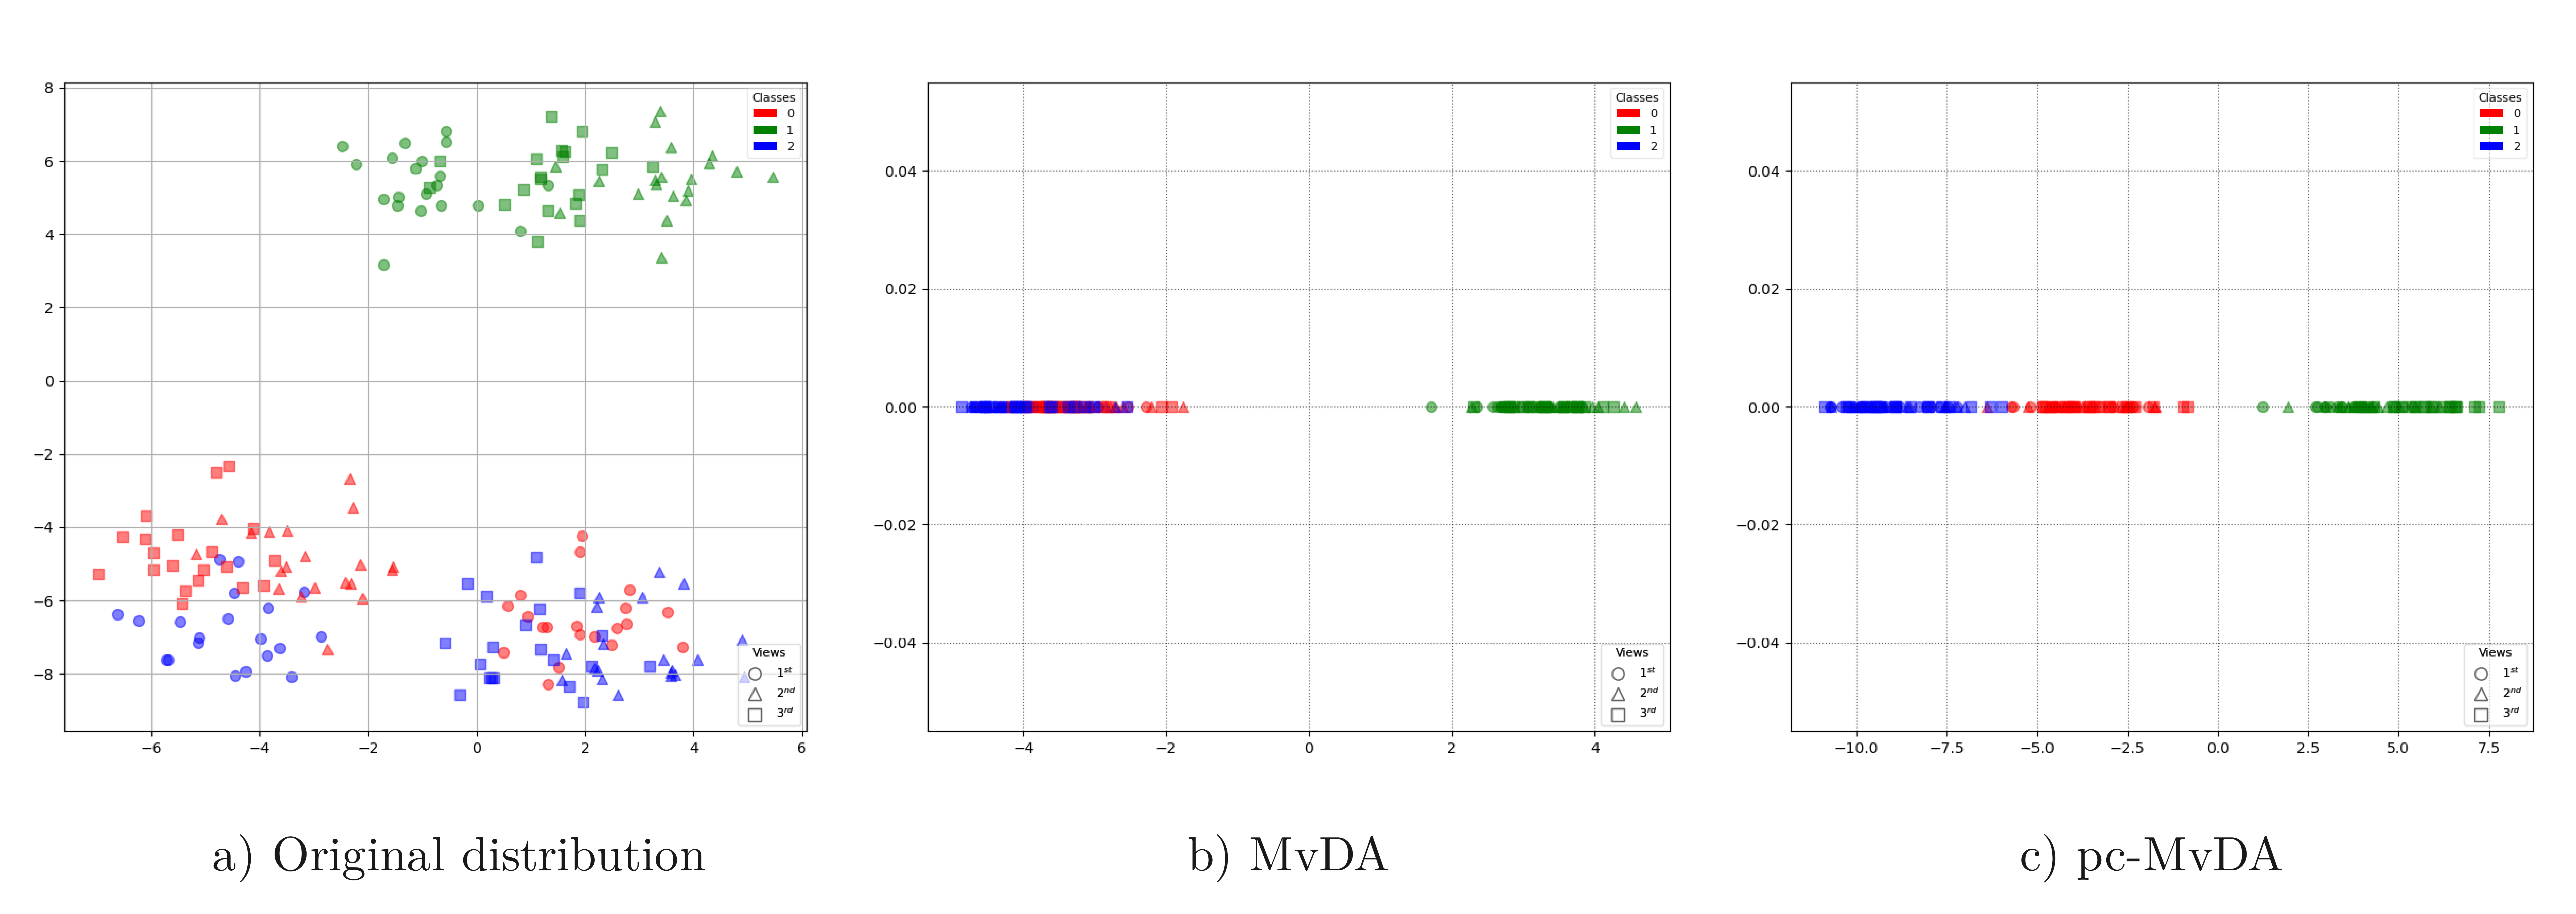
\includegraphics[width=1\linewidth]{Figs/Synthetic1.png}
        \caption{A synthetic dataset of 180 data points, evenly distributed to 3 classes among 3 different views; a) 2-D original distribution; b) 1-D projection of MvDA; c) 1-D projection of pc-MvDA}
        %\vspace{-0.3cm}
        \label{fig:synthetic1}
    \end{figure}

    \begin{figure}[htbp]
        \centering
        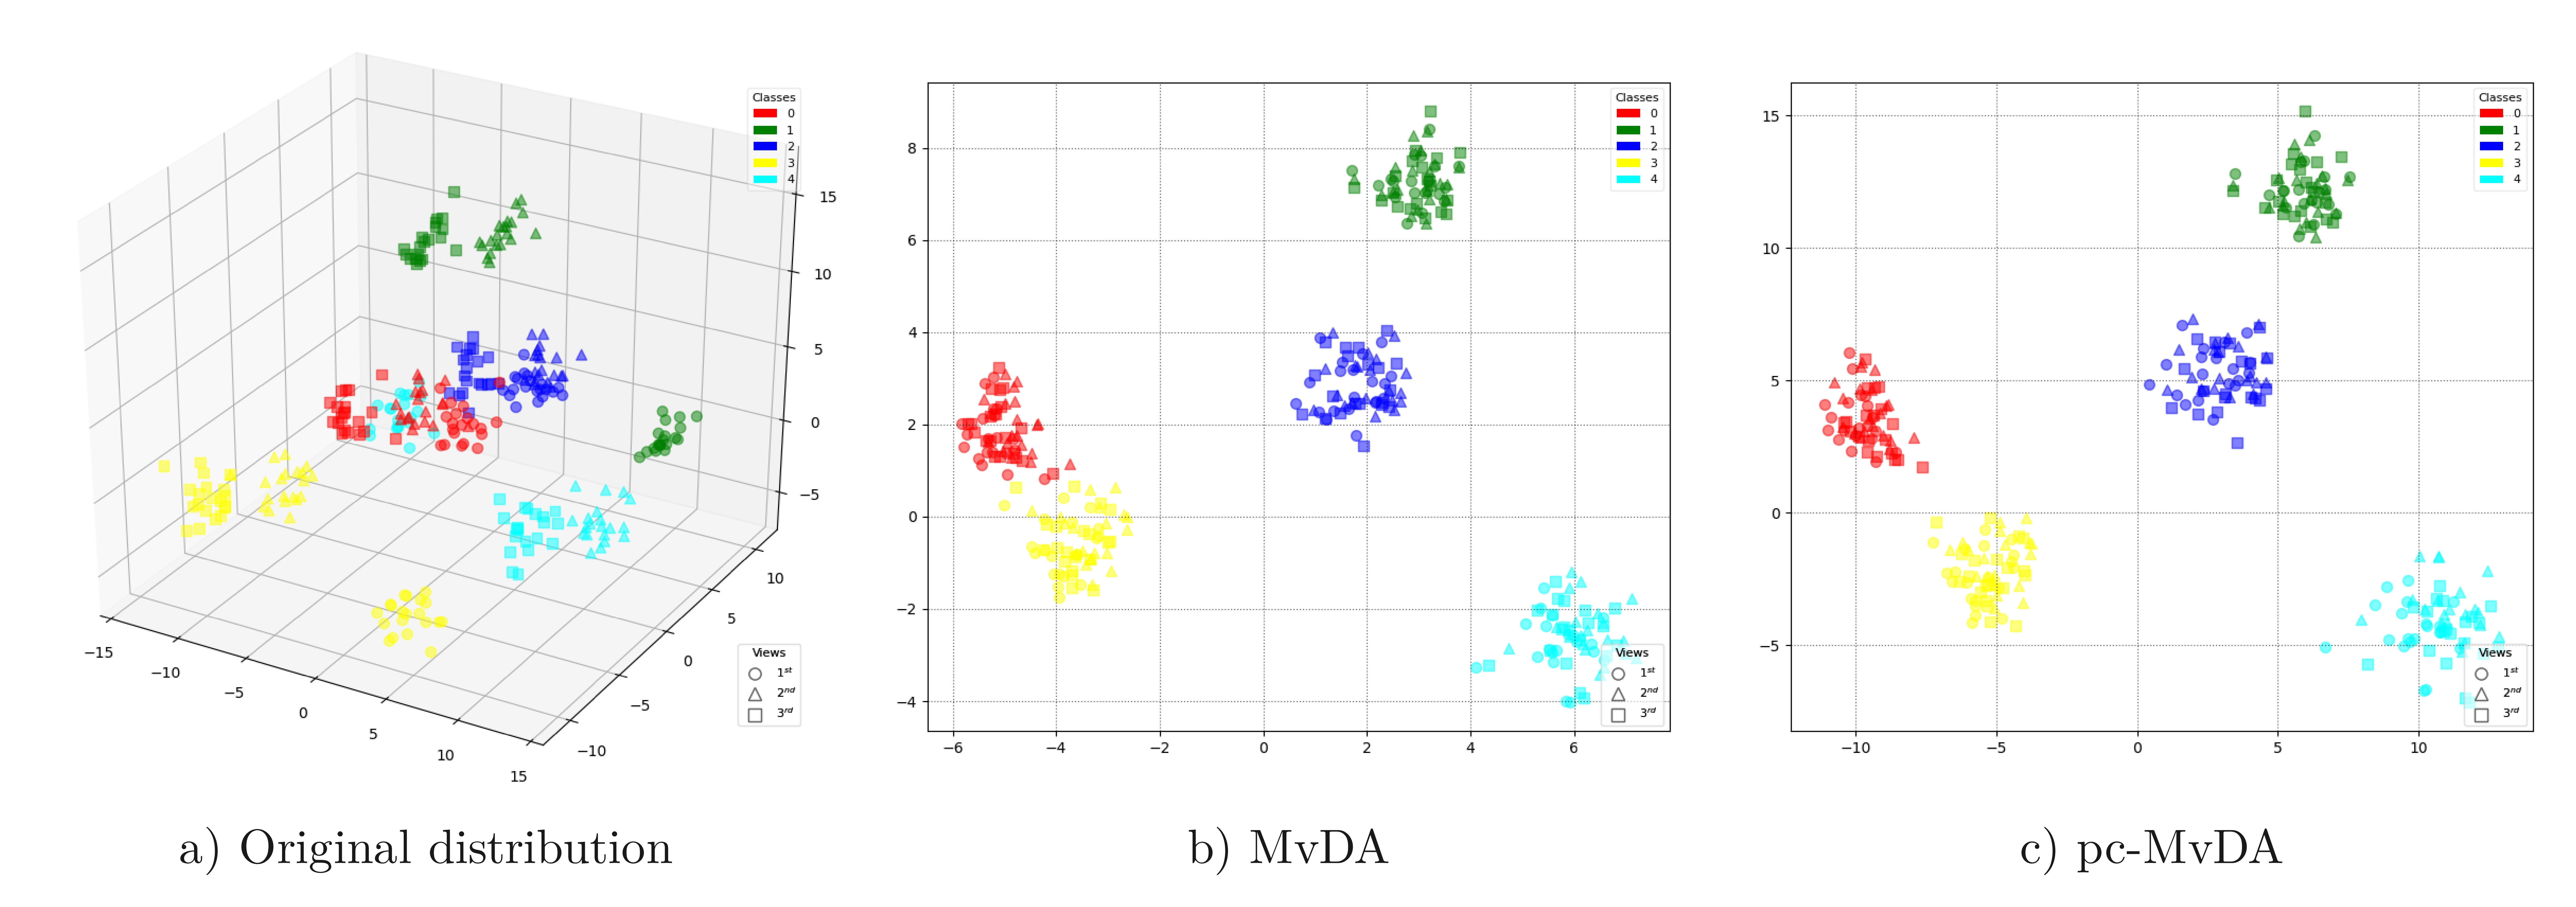
\includegraphics[width=1\linewidth]{Figs/Synthetic2.png}
        \caption{A synthetic dataset of 300 data points, evenly distributed to 5 classes among 3 different views; a) 3-D original distribution; b) 2-D projection of MvDA; c) 2-D projection of pc-MvDA}
        %\vspace{-0.3cm}
        \label{fig:synthetic2}
    \end{figure}



    \section{Summary}
        The novel human action and gesture recognition framework was introduced in this chapter, which consists of two components.
        Firstly, convolutional based clip-level extraction using either 2D CNN (i.e. ResNet) combined with temporal modeling techniques (AP, RNN, TA) or 3D CNN (i.e. C3D, ResNet 3D) are trained separately for each view.
        In the later stage, multi-view analysis algorithms (including pc-MvDA - the main contribution of this thesis) are employed to project common features space, in which the final classification process take place.
        The new formulation of pc-MvDA successfully enforces class separability by adding pairwise distance constraint and casting the final objective to an efficient gradient descent optimization problem that can theoretically be backpropagated to previous layers of CNN feature extractors.
        However, the framework is currently not easily end-to-end trainable due to enormous size of multiple deep feature extractors coupled with the problematic prerequisite of knowing class means when using multi-view analysis as loss function.

    %!TEX root = ../../main.tex

\chapter{Experiments} \label{chap:experimental_result}
    \section{Introduction}
        This chapter represents the methodology proposed in this thesis.
        In section \ref{sec:datasets} and section \ref{sec:protocol}, the benchmarking datasets and evaluation protocol used in experiments of this thesis will be listed out.
        Section \ref{sec:experimental_setup} gives details about the programming configurations of the experiments.
        And finally, section \ref{sec:results} shows the experimental outcomes of proposed framework, compares them with results reported in existing publications and gives discussion.

    %!TEX root = ../../../main.tex

\section{Datasets} \label{sec:datasets}

    In this thesis, three datasets are used in evaluation of the proposed algorithm. Two of which are benchmark datasets IXMAS \cite{weinland2006free}, MuHAVi \cite{murtaza2016multi} and the other (namely MICAGes) is recorded at computer vision department of MICA Institute. 

    %!TEX root = ../../../main.tex

\subsection{IXMAS dataset}
    The IXMAS dataset is a multi-view dataset built by Perception project \cite{weinland2006free}.
    It contains 12 action classes (check watch, cross arms, scratch head, sit down, get up, turn around, walk, wave, punch, kick, point and pick up) recorded simultaneously by 5 cameras (4 side view cameras and 1 top view camera).
    Each action is performed 3 times by 10 actors (5 males / 5 females).
    Some representative frames of action \textit{check watch} are shown in Fig.\ref{Fig:IXMAS1}.

    \begin{figure}[h]
        \centering
        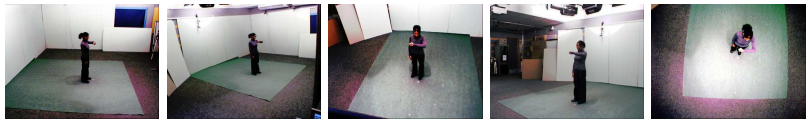
\includegraphics[width=1\linewidth]{figs/IXMAS1.png}
        \caption{Illustration of frames extracted from action \textit{check watch} observed from five camera viewpoints.}
        %\vspace{-0.3cm}
        \label{Fig:IXMAS1}
    \end{figure}

    During the time of writing this thesis, the original version of the dataset is no longer publicly available due to the privacy issues.
    Only a subset of 1692 samples containing samples from four side camera views (excluding the top down view) that have been downloaded previously was utilized with the agreement of the data-set's authors.
    The comparison with SOTA methods on this dataset will only be taken from the four side view cameras. 

    %!TEX root = ../../../main.tex

\subsection{MuHAVi dataset}
    The MuHAVi dataset is constructed and introduced by \cite{murtaza2016multi}. It is usually referred as MuHAVi-uncut because it contains full, raw videos of 17 actions, asynchronously captured by eight cameras that provide completely overlapping coverage of a rectangular action zone from different viewing directions as in Fig.\ref{Fig:MuHAVi1}. 

    \begin{figure}[h]
        \centering
        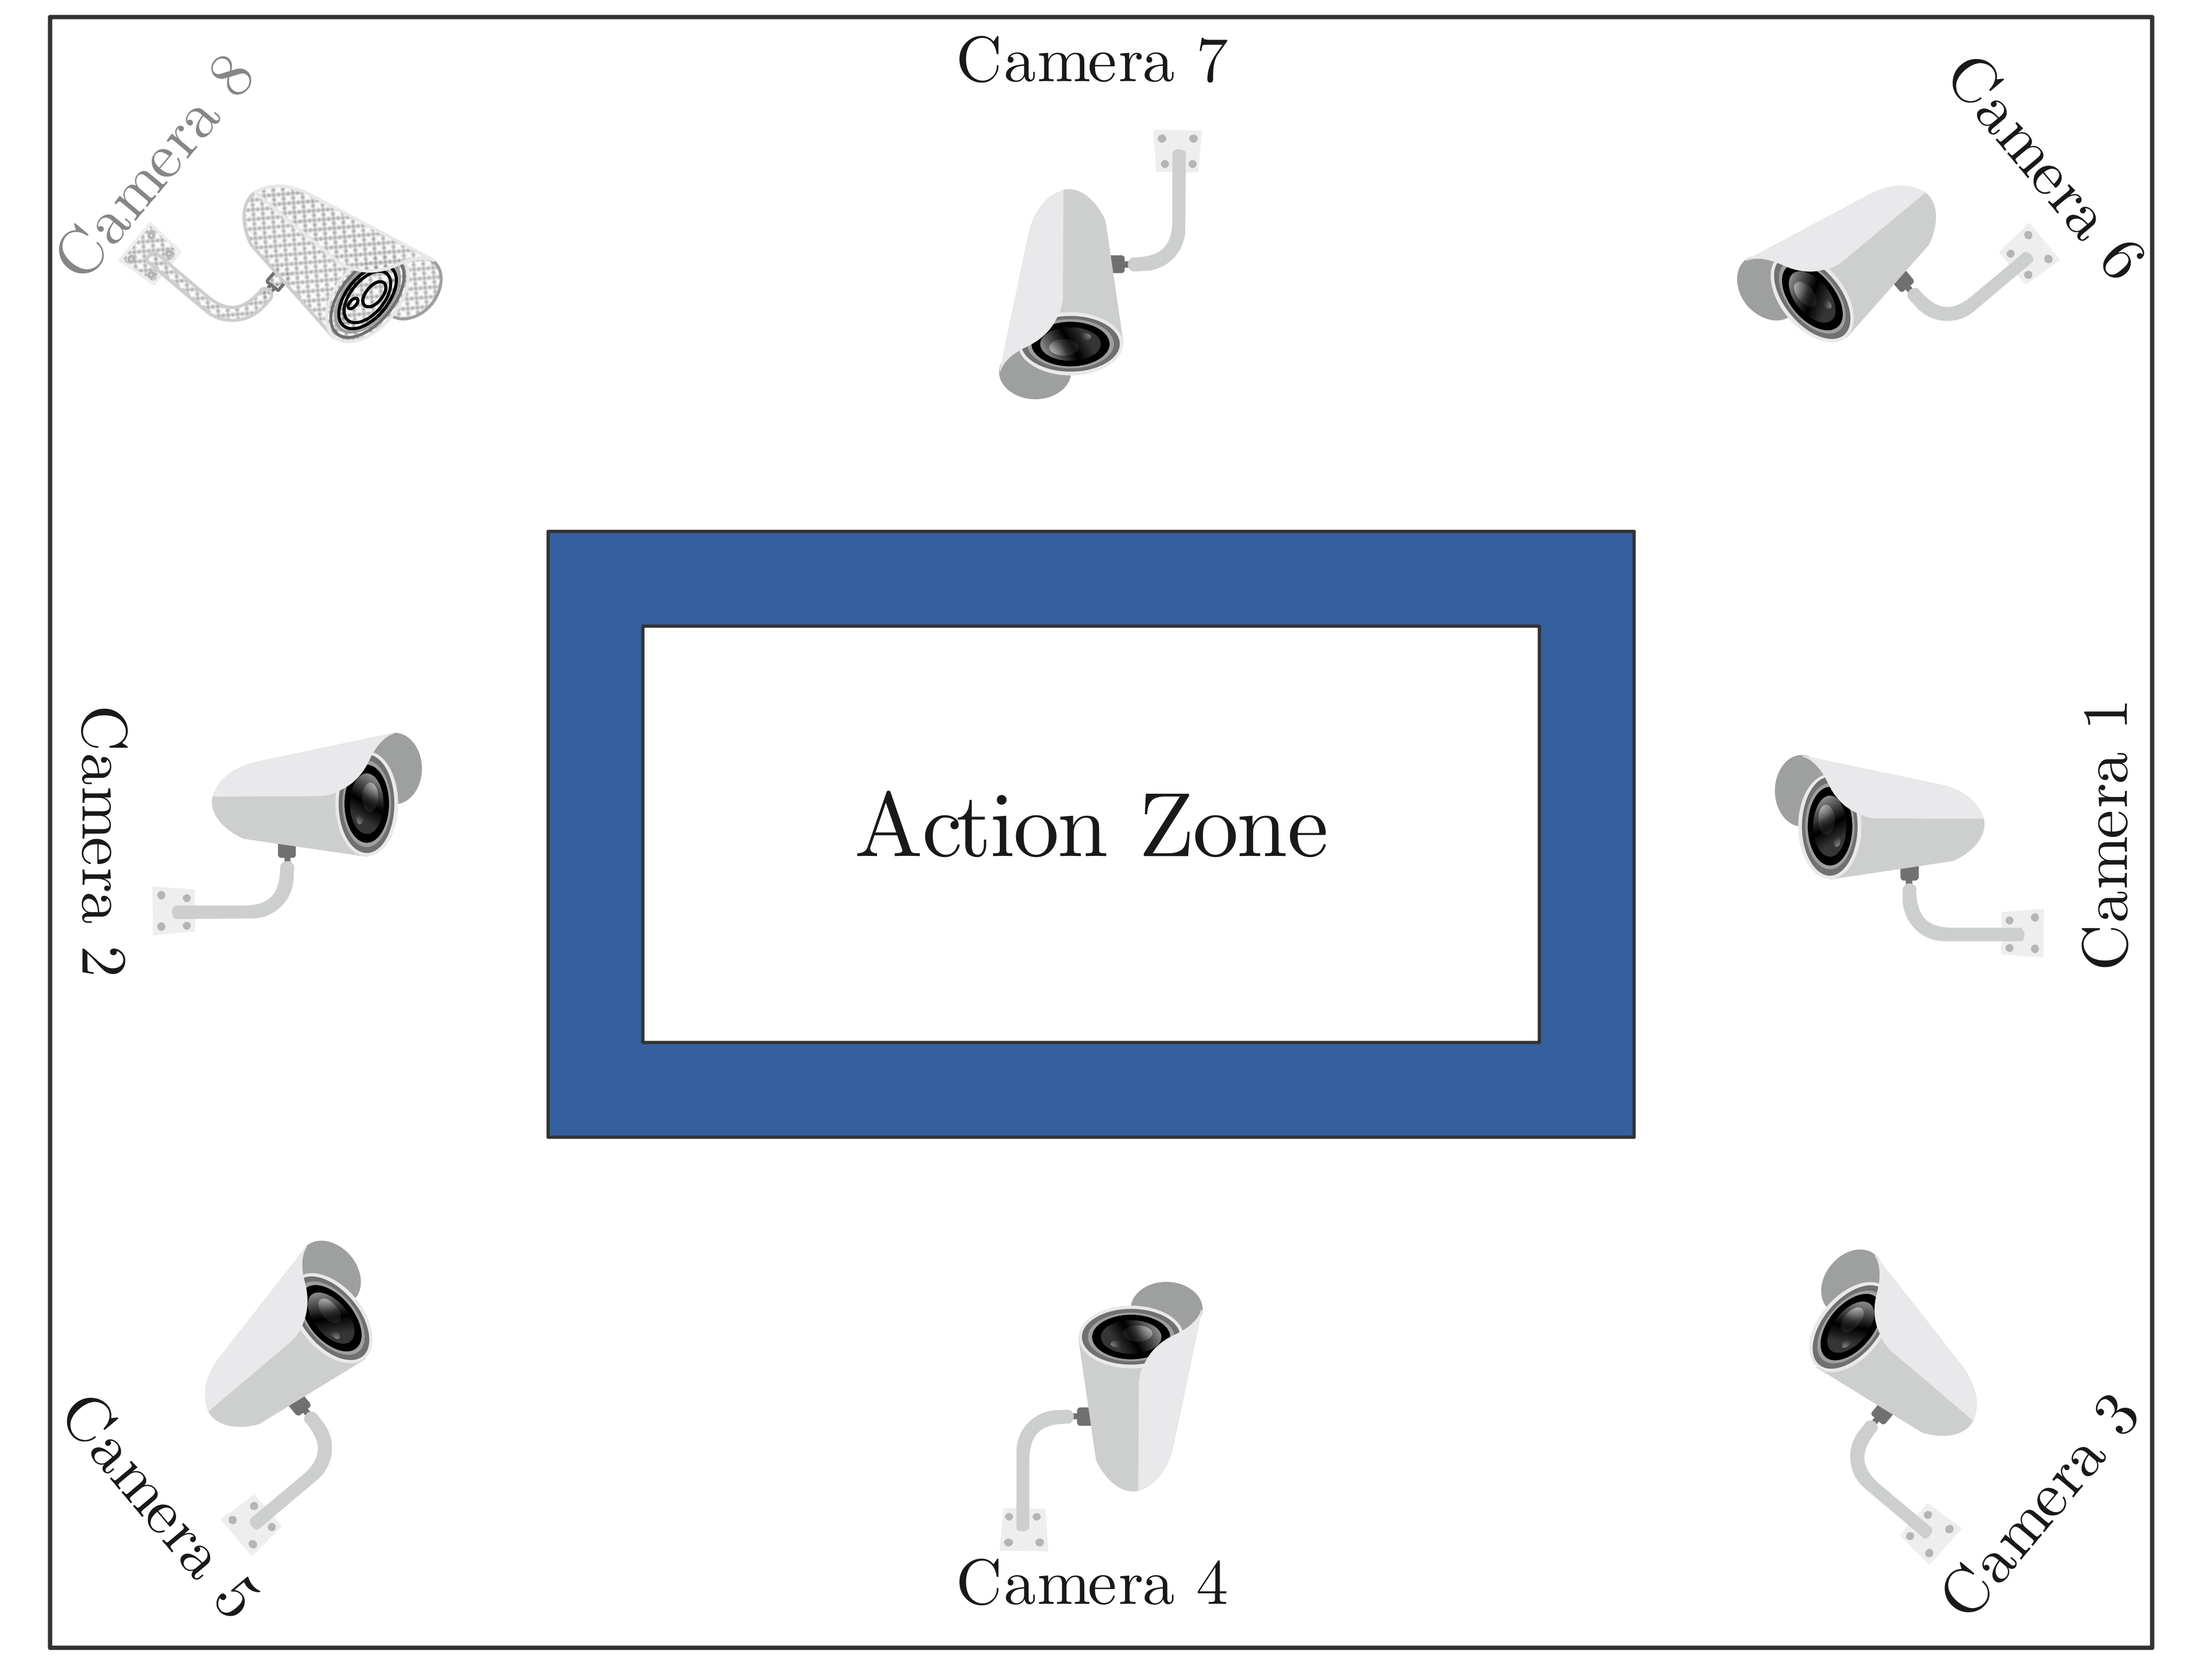
\includegraphics[width=0.8\linewidth]{figs/MuHAVi1.png}
        \caption{Environment setup to collect action sequences from 8 views \cite{murtaza2016multi}.}
        %\vspace{-0.3cm}
        \label{Fig:MuHAVi1}
    \end{figure}

    The actions are are walk turn back, run stop, punch, kick, shotgun collapse, pull heavy object, pickup throw object, walk fall, look in car, crawl on knees, wave arms, draw graffiti, jump over fence, drunk walk, climb ladder, smash object, and jump over gap. 
    Each was performed several times by 7 actors (5 males / 2 females). 
    The videos were collected at rate of 25 fps with resolution of 720 $\times$ 576, except for the $8^{th}$ camera whose data is not included in experiments of this thesis due to absence of annotation.
    Some representative frames of action \textit{punch} are shown in Fig.\ref{Fig:MuHAVi2}.

    \begin{figure}[htbp]
        \centering
        \includegraphics[width=1\linewidth]{figs/MuHAVi2.png}
        \caption{Illustration of frames extracted from an action \textit{punch} observed from Camera 1 to Camera 7.}
        %\vspace{-0.3cm}
        \label{Fig:MuHAVi2}
    \end{figure}

    %!TEX root = ../../../main.tex

\subsection{MICAGes dataset}
    There does not exist a dataset publicly available in the literature which is dedicated to the evaluation of robustness of hand gesture recognition w.r.t. viewpoint changes.
    Therefore, thanks to the work of computer vision department at MICA Institute, a dataset was carefully designed and collected from multiple viewpoints in indoor environment with complex background.
    It consists of 9 dynamic hand gestures which correspond to control commands of electronic home appliances.
    Each gesture is a combination of hand movement following a pre-defined direction and changing of hand shape in a natural manner.

    Five Kinect sensors {K1, K2, K3, K4, K5} are setup at five positions in a square simulation room of $16m^2$ (Figure \ref{Fig:MICAGes1}).
    This work aims to capture hand gestures under multiple viewpoints synchronously. The subjects are invited to stand at a fixed position approximately 2 meters in front of the center view.
    The Kinect sensors provide both RGB and Depth data recorded at frame rate of 20 fps and resolution of 640 $\times$ 480, which legitimates the capture a multi-view and multi-modal dataset.

    \begin{figure}[h]
        \centering
        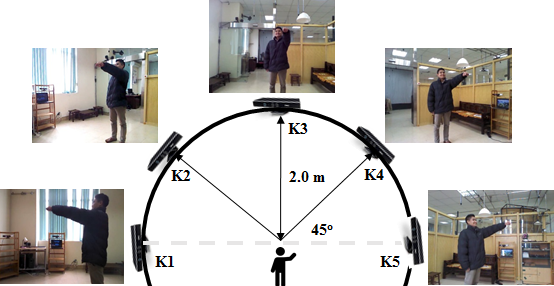
\includegraphics[width=0.8\linewidth]{figs/MICAGes1.png}
        \caption{Environment setup to capture MICAGes dataset.}
        %\vspace{-0.3cm}
        \label{Fig:MICAGes1}
    \end{figure}

    Twelve participants (08 males / 04 females) are voluntary to perform gestures one after another, each gesture three times.
    In the experiments of this thesis, only RGB information is concerned.
    Totally, the dataset contains 1620 (5 views $\times$ 9 gestures $\times$ 12 subjects $\times$ 3 times) dynamic hand gestures.
    Illustrations of segmented hand poses of a gesture are shown in Figure \ref{Fig:MICAGes2}.

    \begin{figure}[htbp]
        \centering
        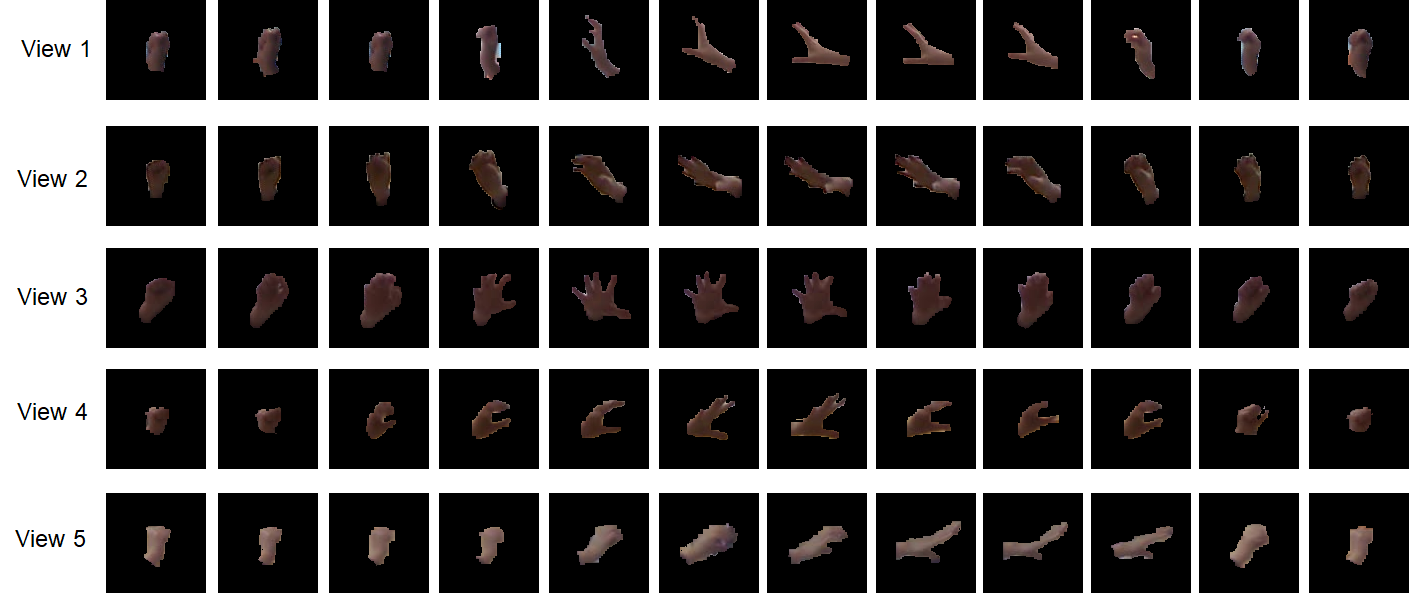
\includegraphics[width=0.9\linewidth]{figs/MICAGes2.png}
        \caption{Illustration of a gesture belonging to the $6^{th}$ class observed from 5 different views.}
        %\vspace{-0.3cm}
        \label{Fig:MICAGes2}
    \end{figure}


    %!TEX root = ../../main.tex

\section{Evaluation Protocol} \label{sec:protocol}
    The leave-one-actor out cross validation strategy represented in \cite{Stone1974} is employed and average accuracy (\%) are computed as means of comparison.
    In order to evaluate the proposed framework in terms of cross-view performance, it is further combined with cross-view validation.
    That means at a moment only two views are picked to evaluate, each consists of a train and a test part defined by the leave-one-actor out strategy.
    Apart from the proposed evaluation protocol, from now named ``\emph{protocol 1}'', another ``\emph{protocol 2}'' is assessed, which is regularly used in the literature.
    The main difference is in second protocol, the notation of train or test is omitted after feature extraction stage, every features samples from single view are included to train the multi-view metrics, then the classifier is fit on common features of one view and tested on common features of another view.
    It is noticed that the first evaluation protocol is more challenging because the in the second protocol, the constructed common space is already fit on the whole multi-view dataset. As a result, the later predictive models are trained and evaluated on features generated by a severely over-fitted projector. % Details about two evaluation protocols is presented in supplemental materials. 
    The difference between two protocols are illustrated in Figure \ref{Fig:ep}. 

    \begin{figure}[htbp]
      \centering
      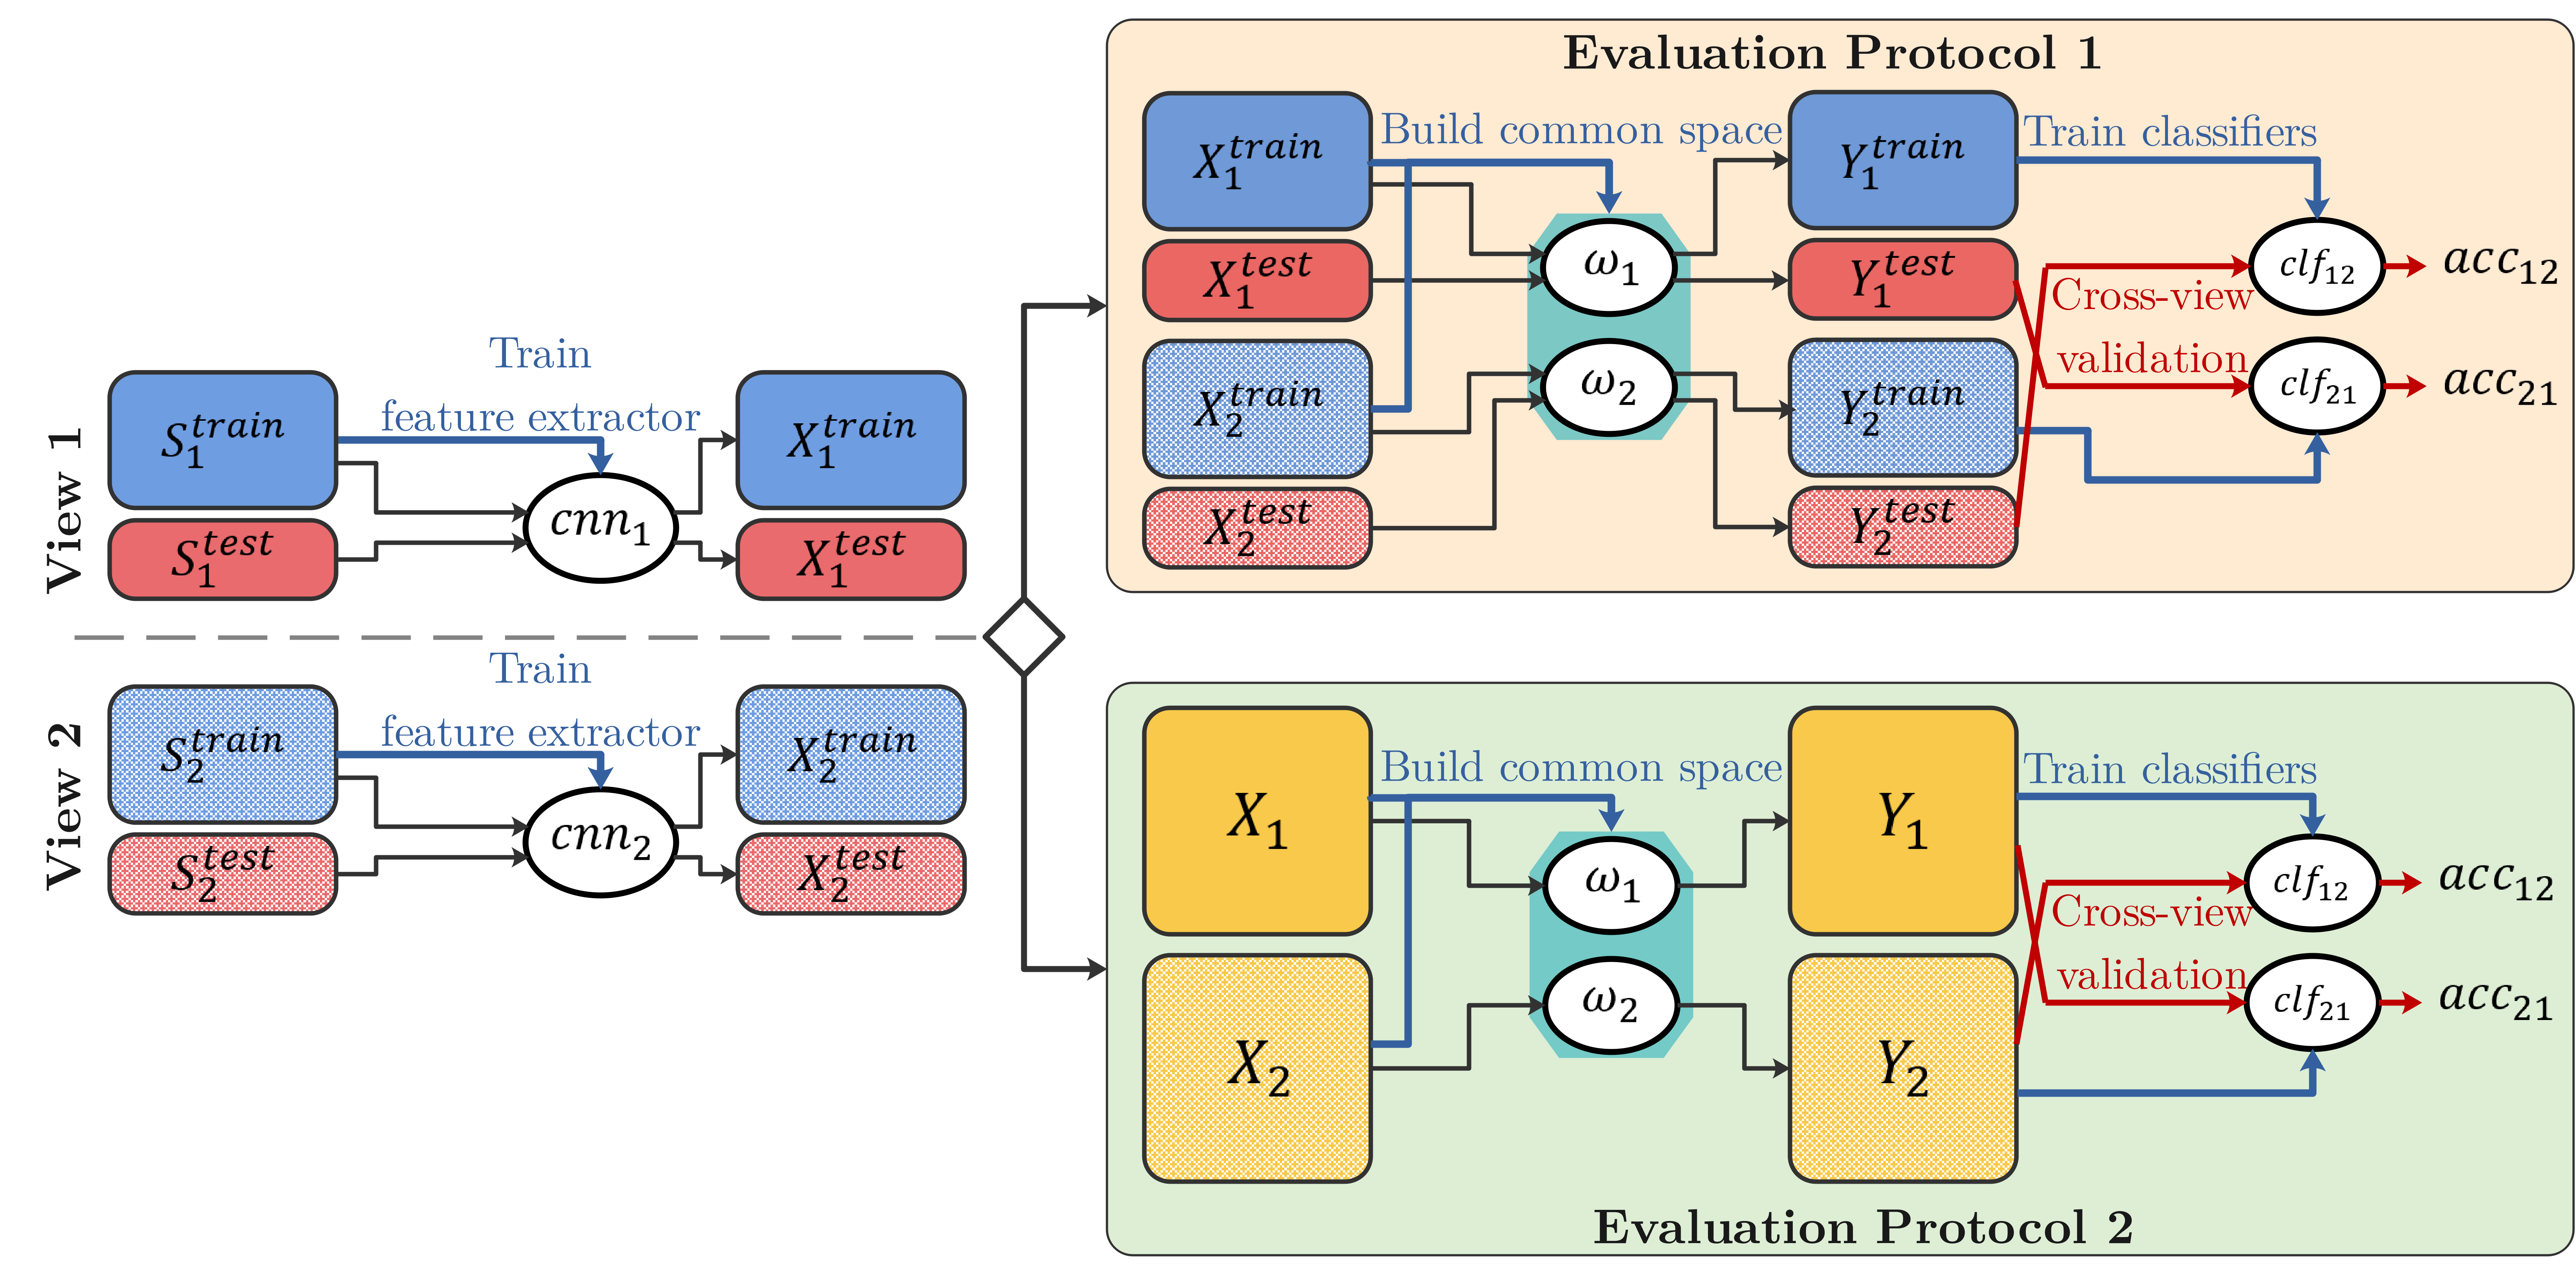
\includegraphics[width=1\linewidth]{figs/protocol.png}
      \caption{Two evaluation protocols used in experiments.}
        %\vspace{-0.3cm}
      \label{Fig:ep}
    \end{figure}
    The overall cross-view evaluation score is computed as average of all evaluation scores of each split, whose method of computation is described specifically in Figure \ref{Fig:ep}:
    \begin{equation}
        {acc}_{ij} = \frac{\sum_{k=1}^M {acc}^{(k)}_{ij}}{M}
    \end{equation}
    where M is the number of actors. Both protocols finally generate a cross-view accuracy matrix as follows:
    \begin{equation}
        \left[\begin{matrix}{acc}_{11}&{acc}_{12}&\cdots&{acc}_{1v}\\{acc}_{21}&{acc}_{22}&\cdots&{acc}_{2v}\\\vdots&\vdots&\ddots&\vdots\\{acc}_{v1}&{acc}_{v2}&\cdots&{acc}_{vv}\\\end{matrix}\right]
        \label{eq:multi-view_scores}
    \end{equation}
    For eager expression, let's define function $\operatorname{accuracy}\left(Y, \tilde{Y}\right)$ as the accuracy score when fitting a classifier on $Y$ features and evaluating its prediction on $\tilde{Y}$ features. Each cell can be expressed accordingly:
    \begin{align}
        {score}_{jr}^{\boldsymbol{protocol 1}} & =\left<\left\{\operatorname{accuracy}\left(Y_j^{train},Y_r^{test}\right)\middle|\ j,r=(1,..,v)\right\}\right> \\
        {score}_{jr}^{\boldsymbol{protocol 2}} & =\left<\left\{\operatorname{accuracy}\left(Y_j,Y_r\right)\middle|\ j,r=(1,..,v)\right\}\right>
    \end{align}

    \textbf{Multi-view strategy:} As MvDA and its variants can theoretically scale for an arbitrary number of views, in order to fairly compare the proposed algorithm with others that only apply for 2 views, I also experiment 2 different multi-view strategies. The key idea is that each strategy restricts the number of views participated in the training process of MvA algorithms.

    In ``\emph{multi-view}'' strategy, only one set of $W^*=\left\{{\omega}_1, {\omega}_2, ..., {\omega}_v\right\}$ is learnt and all separated view features are transformed $Y_j=\omega_j^TX_j,\ j=(1,...,v)$ before computation of accuracy.

    In ``\emph{cross-view}'' strategy, each cell ${score}_{jr}$ of \eqref{eq:multi-view_scores} must be calculated exclusively with the inclusion of only features of those views $j$ and $r$ (wihtout information from other views).
    Therefore, for each distinct combination $jk$, $W_{jr}^*=\left\{{\omega}_j, {\omega}_r\right\}$ is learnt to transform $X_j$ and $X_r$. The diagonal of \eqref{eq:multi-view_scores} is also ignored in this strategy.

    Since there are many scores generated by such extra complicated cross validation process when cycling through every actors, the final reported is average of all.
    Further, it is noticed that in existing works, the evaluation have been done mostly similar to the second evaluation protocol. Hence, in comparison with state of the art techniques, only the scores resulted from the second evaluation protocol are taken.

    %!TEX root = ../../main.tex

\section{Experimental Setup} \label{sec:experimental_setup}
    \subsection{Programming Environment and Libraries}
        The majority of my code implementation is written in Python, fueled by PyTorch \cite{NEURIPS2019_9015} deep learning framework.
        The framework offers powerful supports for matrix manipulation, automatic diffirentiation, accelerated training of deep neural networks on parallel computing platforms and flexibility to efficiently research new algorithmic approaches.
        The MvDA and MvDA-vc Matlab implementations are inherited from the repository published by \cite{kan2015multi} with slight modifications.
        The implementation of proposed pc-MvDA is published at \github{https://github.com/inspiros/pcmvda}.

    \subsection{Configurations}
        \paragraph{Feature extractors}
        All models are trained for 60 epoches with SGD optimizer, initial learning rate is 0.0003 and momentum is 0.9.
        The choosen pre-trained models are:
        \begin{itemize}
            \item{ResNet-50} model was pre-trained on ImageNet dataset and is available in subpackage \textit{torchvision.models} of PyTorch.
            \item{C3D} model was pre-trained on Sports-1M \cite{karpathy2014large} then fine-tuned on Kinetics dataset \cite{kay2017kinetics}. The model is implemented by \cite{VMZ} in Caffe2 deep learning framework, which was improved from original model presented in \cite{tran2015learning} by inserting Batch Normalization layers after each Convolution layer.
            \item{ResNet-50 3D} was pre-trained on Kinetics dataset and weights are given by \cite{hara2018can}.
        \end{itemize}

        \paragraph{Multi-view analysis algorithms}
        Output dimensions of both algorithms are 200. MvDA has no alterable parameter and $\lambda$ of view-consistency term in MvDA-vc is set to 0.03.
        For pc-MvDA, the hyperparameters are $\beta = 1$ and $q = 1$ and the optimizer utilized is Adam with initial learning rate set to 0.01, on each experiment trained 300 epochs.

        \paragraph{Classifier}
        For comparison with related methods, the final classifier used is kNN with $k = 1$.

    %!TEX root = ../../../main.tex

\section{Experimental Results and Discussions}
    %!TEX root = ../../../main.tex

\subsection{Experimental results on IXMAS dataset}
    \paragraph{1) Cross-view validation:} In this experiment, I train on data from one view (training view) and testing on data from another view (testing view) then compute the accuracies for two evaluation protocols. Table \ref{tab:cross_p1_ixmas} shows comparative results of using different deep features (C3D, ResNet-50 3D, ResNet-50 RNN, ResNet-50 TA, ResNet-50 AP) and multi-view discriminant analysis techniques (MvDA, MvDA-vc and my proposed pc-MvDA). 

    With the first evaluation protocol, the proposed pc-MvDA, when combined with deep features, gives mostly best accuracy for both evaluation protocols. With C3D features, accuracy by pc-MvDA (88.43\%) is 6.6\% higher than MvDA (81.84\%). pc-MvDA is even better than MvDA-vc (2.87\%). pc-MvDA achieved higher accuracy (about 6\% higher) than MvDA and MvDA-vc with ResNet-50 TA and ResNet-50 AP features. In average, pc-MvDA is 3.09\% higher than MvDA and 1.4\% higher than MvDA-vc.
    
    \begin{table}[htbp]
    \centering
    \caption{Cross-view recognition comparison on IXMAS dataset}
    \resizebox{0.8\textwidth}{!}{
    \begin{tabular}{|l|c|c|c|c|c|c|}
        \hline
        \multirow{2}{*}{Deep features}          & \multicolumn{3}{c|}{Protocol 1}   & \multicolumn{3}{c|}{Protocol 2}           \\ \cline{2-7} 
                                                & MvDA  & MvDA-vc & pc-MvDA         & MvDA  & MvDA-vc        & pc-MvDA          \\ \hline
        \multicolumn{1}{|c|}{C3D}               & 81.84 & 85.56   & \textbf{88.43}  & 96.54 & 99.29          & \textbf{99.98}   \\ \hline
        \multicolumn{1}{|c|}{ResNet-50 3D}      & 91.25 & 92.19   & \textbf{92.89}  & 97.30 & \textbf{99.73} & 99.65            \\ \hline
        \multicolumn{1}{|c|}{ResNet-50 RNN}     & 75.51 & 76.12   & \textbf{76.54}  & 99.99 & 99.71          & \textbf{100}     \\ \hline
        \multicolumn{1}{|c|}{ResNet-50 TA}      & 79.44 & 80.58   & \textbf{82.05}  & 99.33 & 99.34          & \textbf{99.84}   \\ \hline
        \multicolumn{1}{|c|}{ResNet-50 AP}      & 77.00 & 79.04   & \textbf{80.58}  & 99.68 & 99.81          & \textbf{99.92}   \\ \hline
    \end{tabular}}
    \label{tab:cross_p1_ixmas}
    \end{table}

    For the second evaluation protocol, pc-MvDA almost always keeps better performance compared to MvDA and MvDA-vc. The recognition accuracy scores obtained by both pc-MvDA and MvDA-vc are nearly 100\% for every kind of deep features. With C3D features and ResNet-50 3D features, pc-MvDA is 99.98\% and 99.65\%, which is 3.44\% and 2.35\% higher than the orginal MvDA (96.54\% and 97.3\%) respectively. In average, pc-MvDA is 1.31\% better than MvDA and 0.3\% better than MvDA-vc. 

    In terms of deep features, with the first evaluation protocol, ResNet-50 3D gives the best accuracy (92.89\%) following by C3D (88.43\%), ResNet-50 TA (82.05\%), ResNet-50 AP (80.58\%). The lowest accuracy obtained by ResNet-50 RNN is only 76.54\%. It shows that ResNet-50 3D produces the most discriminative feature space. %Table \ref{tab:cross_feature_ixmas} shows comparative results when using pc-MvDA method with different deep features regarding pairwise views. 

    \begin{table}[htbp]
    \centering
    \caption{Cross-view recognition results of different features on IXMAS dataset with pc-MvDA method. The result in the bracket are accuracies of using features C3D, ResNet-50 3D, ResNet-50 RNN, ResNet-50 TA, Restnet-50 AP respectively. Each row corresponds to training view (from view C0 to view C3). Each column corresponds to testing view (from view C0 to view C3)}
    \resizebox{\textwidth}{!}{\begin{tabular}{|c|c|c|c|c|}
        \hline
        \backslashbox{Training}{Testing} & C0 & C1 & C2 & C3 \\ \hline
        C0 & N/A & (90.7, \textbf{91.9}, 81.6, 84.6, 83.6) & (86.9, \textbf{93.9}, 78.0, 79.6, 78.1) & (89.9, \textbf{93.4}, 76.3, 82.8, 82.1) \\ \hline
        C1 & (86.6, \textbf{91.9}, 71.5, 81.1, 77.5) & N/A & (85.9, \textbf{94.2}, 78.6, 79.3, 80.3) & (88.9, \textbf{93.7}, 74.8, 82.3, 81.3) \\ \hline
        C2 & (87.6, \textbf{92.4}, 72.8, 81.8, 78.5) & (90.7, \textbf{91.7}, 80.6, 83.6, 82.6) & N/A & (89.4, \textbf{93.7}, 75.5, 82.3, 80.6) \\ \hline
        C3 & (87.6, \textbf{92.9}, 70.2, 82.1, 78.8) & (90.7, \textbf{91.2}, 81.6, 84.1, 82.8) & (86.4, \textbf{93.7}, 77.3, 80.6, 80.8) & N/A \\ \hline
    \end{tabular}}
    \label{tab:cross_feature_ixmas}
    \end{table}

    \paragraph{2) Multi-view validation} Table \ref{tab:ixmas_multi} shows multi-view recognition results. The conclusion is consistent with the case of cross-view evaluation: ResNet-50 3D is the best feature extractor. When it is combined with pc-MvDA, the framework gives the highest accuracy for the first protocol (92.82\%), following by C3D (88.19\%), ResNet-50 TA (81.49\%), ResNet-50 AP(80.43\%), and ResNet-50 RNN (76.47\%). Both MvA algorithms give similar accuracies for the second evaluation protocols (nearly 100\%). Again, pc-MvDA enhances the performance of MvDA by 2.43\% for the first protocol and 0.83\% for the second protocol. It only gives slightly better result than MvDA-vc (0.83\% for the first protocol and 0.74\% for the second protocol). 

    \begin{table}[htbp]
    \centering
    \caption{Multi-view recognition comparison on IXMAS dataset}
    \resizebox{0.7\textwidth}{!}{\begin{tabular}{|c|c|c|c|c|c|c|}
        \hline
        \multirow{2}{*}{Deep features}          & \multicolumn{3}{c|}{Protocol 1}   & \multicolumn{3}{c|}{Protocol2}                    \\ \cline{2-7} 
                                                & MvDA  & MvDA-vc & pc-MvDA         & MvDA           & MvDA-vc        & pc-MvDA         \\ \hline
        \multicolumn{1}{|c|}{C3D}               & 86.93 & 87.04   & \textbf{88.19}  & \textbf{99.99} & 99.44          & \textbf{99.98}  \\ \hline
        \multicolumn{1}{|c|}{ResNet-50 3D}      & 91.84 & 92.33   & \textbf{92.82}  & \textbf{100}   & 99.80          & 99,67           \\ \hline
        \multicolumn{1}{|c|}{ResNet-50 RNN}     & 72.44 & 75.95   & \textbf{76.47}  & 99.34          & \textbf{99.97} & \textbf{99.96}  \\ \hline
        \multicolumn{1}{|c|}{ResNet-50 TA}      & 76.74 & 81.01   & \textbf{81.49}  & 95.80          & 98.25          & \textbf{99.79}  \\ \hline
        \multicolumn{1}{|c|}{ResNet-50 AP}      & 79.28 & 78.93   & \textbf{80.43}  & \textbf{100}   & 98.11          & 99.85           \\ \hline
    \end{tabular}}
    \label{tab:ixmas_multi}
    \end{table}

    Figure \ref{fig:pc-MvDA_confusion_ixmas} compares the performance of feature extractors regarding each action class in multi-view evaluation scheme combined with the first evaluation protocol. There are clear margins between the performance of ResNet-50 3D and followed by C3D with other types of deep features, especially in harder actions (the first class to the third class and the eighth class to the eleventh class). These actions (check watch, cross arm, scratch head, wave, punch, kick, point) involve the most part static pose of the body and only movement of limbs, whereas other actions 4 - sit down, 5 - get up, 6 - turn around, 7 - walk and 12 - pickup include movement of the whole body and are easier to be recognized. This suggests that 3D convolution can better deal with small difference of movement in action images, which in turn generates a much more classification-ready feature space for latter stage of recognition.

    \begin{figure}[htbp]
        \centering
        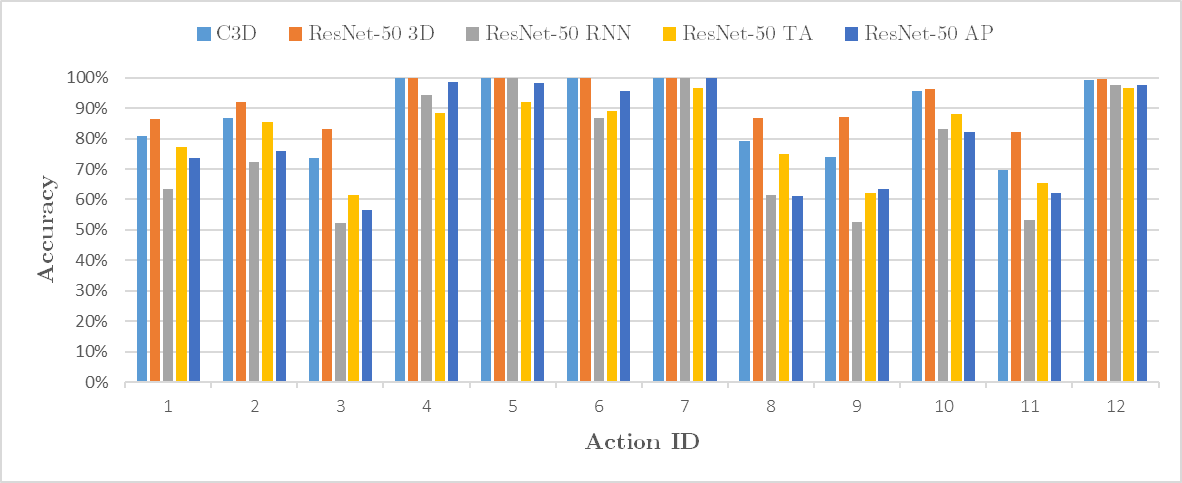
\includegraphics[width=0.8\linewidth]{figs/pc-MvDA_confusion_ixmas.png}
        \caption{Comparison of accuracy on each action class using different deep features combined with pc-MvDA on IXMAS dataset.}
        %\vspace{-0.3cm}
        \label{fig:pc-MvDA_confusion_ixmas}
    \end{figure}

    Table \ref{tab:sota_ixmas} compares the best combination of ResNet-50 3D and pc-MvDA with state-of-the-art frameworks. The comparison is for reference only because in other works, low-level hand-crafted video representation is used as private features and train-test strategy is leave-one-class out, which is not applicable to supervised deep feature extractors in this work. However, the results are still commensurable. % in circumstances where supervised approaches are adopted.
    % TODO - High priority

    \begin{table}[htbp]
    \centering
    \caption{Comparison of proposed methods with SOTA methods on IXMAS dataset according to the second evaluation protocol}
    \resizebox{0.7\textwidth}{!}{
    \begin{tabular}{|c|c|c|}
    \hline
    Methods                                                              & Cross-view & Multi-view \\ \hline
    Liu et al. \cite{liu2011cross}                                   & 76.32      & N/A       \\ \hline
    Zheng et al. \cite{zheng2012cross}                               & 95.1       & 99.32     \\ \hline
    Zheng et al. \cite{zheng2016cross}                               & 97.8       & 99.4      \\ \hline
    Kong et al. \cite{kong2017deeply}                                & 99.92      & 100       \\ \hline
    Ulhaq et al. \cite{ulhaq2017space}                               & 66.82      & 92.47     \\ \hline
    Zhang et al. \cite{zhang2018cross}                               & 84.1       & N/A        \\ \hline
    Liu et al. \cite{liu2018learning}                                & N/A        & 90.3     \\ \hline
    Liu et al. \cite{liu2018hierarchically}                          & 99.95      & 99.67     \\ \hline
    Proposed method (ResNet-50 3D + pc-MvDA)                     & 99.67      & 99.65       \\ \hline
    \end{tabular}}
    \label{tab:sota_ixmas}
    \end{table}

    %!TEX root = ../../../main.tex

\subsection{Experimental results on MuHAVi dataset}
    \paragraph{1) Cross-view validation:} Table.\ref{tab:muhavi_cross} illustrates cross-view recognition results. The proposed pc-MvDA consistently produces a better average accuracy of around 96.19\% for protocol 1, approximately 4.55\% and 1.51\% higher than that of MvDA (91.64\%) and MvDA-vc (94.67\%) respectively.

    \begin{table}[htbp]
    \centering
    \caption{Cross-view recognition comparison on MuHAVi dataset}
    \resizebox{0.8\textwidth}{!}{
    \begin{tabular}{|c|c|c|c|c|c|c|}
        \hline
        \multirow{2}{*}{Deep features}          & \multicolumn{3}{c|}{Protocol 1}   & \multicolumn{3}{c|}{Protocol 2}           \\ \cline{2-7} 
                                                & MvDA  & MvDA-vc & pc-MvDA         & MvDA  & MvDA-vc        & pc-MvDA          \\ \hline
        \multicolumn{1}{|c|}{C3D}               & 92.85 & 95.15   & \textbf{97.65}  & 98.95 & 99.76          & \textbf{100}     \\ \hline
        \multicolumn{1}{|c|}{ResNet-50 3D}      & 97.94 & 99.15   & \textbf{99.18}  & 96.77 & \textbf{99.94} & \textbf{99.94}   \\ \hline
        \multicolumn{1}{|c|}{ResNet-50 RNN}     & 95.54 & 95.14   & \textbf{96.18}  & 98.70 & 99.05          & \textbf{99.99}   \\ \hline
        \multicolumn{1}{|c|}{ResNet-50 TA}      & 85.80 & 88.95   & \textbf{91.12}  & 96.57 & 97.03          & \textbf{99.88}   \\ \hline
        \multicolumn{1}{|c|}{ResNet-50 AP}      & 86.09 & 94.98   & \textbf{96.82}  & 89.04 & 98.62          & \textbf{99.93}   \\ \hline
    \end{tabular}}
    \label{tab:muhavi_cross}
    \end{table}

    %Results in Table.\ref{tab:cross_feature_muhavi} show that our combination with ResNet-50 3D has the highest accuracies in almost every circumstances, even though both features coupled with our proposed pc-MvDA give satisfactory performance with all scores exceeding 91\%.

    \begin{table}[htbp]
    \centering
    \caption{Cross-view recognition results of different features on MuHAVi dataset with pc-MvDA method. The result in the bracket are accuracies of using features C3D, ResNet-50 3D, ResNet-50 RNN, ResNet-50 TA, ResNet-50 AP respectively. Each row corresponds to training view (from view C1 to view C7). Each column corresponds to testing view (from view C1 to view C7)}
    \resizebox{\textwidth}{!}{\begin{tabular}{|c|c|c|c|c|c|c|c|}
        \hline
        \backslashbox{Training}{Testing} & C1 & C2 & C3 & C4 & C5 & C6 & C7 \\ \hline
        C1 & N/A & \begin{tabular}{@{}c@{}} (96.1, \textbf{100}, 96.8, \\ 88.5, 98.5) \end{tabular} & \begin{tabular}{@{}c@{}} (98.6, \textbf{99.6}, 96.6, \\ 88.9, 96.3) \end{tabular} & \begin{tabular}{@{}c@{}} (98.6, \textbf{99.6}, 98.0, \\ 93.1, 98.2) \end{tabular} & \begin{tabular}{@{}c@{}} (97.7, \textbf{99.6}, 95.4, \\ 91.3, 96.1) \end{tabular} & \begin{tabular}{@{}c@{}} (97.7, \textbf{98.4}, 92.3, \\ 93.1, 96.3) \end{tabular} & \begin{tabular}{@{}c@{}} (98.2, \textbf{98.5}, 97.2, \\ 89.8, 97.1) \end{tabular} \\ \hline
        C2 & \begin{tabular}{@{}c@{}} (95.6, \textbf{99.0}, 95.2, \\ 91.3, 95.5) \end{tabular} & N/A & \begin{tabular}{@{}c@{}} (98.9, \textbf{99.6}, 96.9, \\ 90.3, 96.1) \end{tabular} & \begin{tabular}{@{}c@{}} (98.4, \textbf{99.6}, 97.6, \\ 92.6, 98.2) \end{tabular} & \begin{tabular}{@{}c@{}} (97.7, \textbf{99.6}, 95.4, \\ 90.9, 96.1) \end{tabular} & \begin{tabular}{@{}c@{}} (97.8, \textbf{98.4}, 92.7, \\ 93.6, 96.5) \end{tabular} & \begin{tabular}{@{}c@{}} (98.6, \textbf{99.0}, 97.4, \\ 90.6, 96.9) \end{tabular} \\ \hline
        C3 & \begin{tabular}{@{}c@{}} (96.1, \textbf{99.0}, 95.6, \\ 90.3, 95.1) \end{tabular} & \begin{tabular}{@{}c@{}} (97.0, \textbf{100}, 96.7, \\ 88.4, 97.8) \end{tabular} & N/A & \begin{tabular}{@{}c@{}} (98.1, \textbf{99.2}, 98.2, \\ 92.8, 98.2) \end{tabular} & \begin{tabular}{@{}c@{}} (97.9, \textbf{99.6}, 95.4, \\ 90.2, 95.6) \end{tabular} & \begin{tabular}{@{}c@{}} (97.9, \textbf{98.2}, 93.0, \\ 94.2, 96.5) \end{tabular} & \begin{tabular}{@{}c@{}} (97.8, \textbf{98.7}, 97.4, \\ 89.4, 97.6) \end{tabular} \\ \hline
        C4 & \begin{tabular}{@{}c@{}} (96.4, \textbf{98.8}, 95.4, \\ 89.6, 95.3) \end{tabular} & \begin{tabular}{@{}c@{}} (96.3, \textbf{100}, 96.6, \\ 91.0, 98.5) \end{tabular} & \begin{tabular}{@{}c@{}} (98.6, \textbf{99.6}, 97.3, \\ 89.5, 96.1) \end{tabular} & N/A & \begin{tabular}{@{}c@{}} (97.7, \textbf{99.4}, 95.6, \\ 91.3, 96.1) \end{tabular} & \begin{tabular}{@{}c@{}} (\textbf{98.4}, 98.0, 93.2, \\ 93.8, 95.6) \end{tabular} & \begin{tabular}{@{}c@{}} (97.7, \textbf{98.7}, 97.4, \\ 91.3, 96.7) \end{tabular} \\ \hline
        C5 & \begin{tabular}{@{}c@{}} (95.9, \textbf{99.0}, 95.6, \\ 91.3, 95.5) \end{tabular} & \begin{tabular}{@{}c@{}} (96.6, \textbf{100}, 97.1, \\ 89.9, 98.3) \end{tabular} & \begin{tabular}{@{}c@{}} (98.8, \textbf{99.4}, 96.8, \\ 90.7, 96.1) \end{tabular} & \begin{tabular}{@{}c@{}} (98.4, \textbf{99.6}, 98.0, \\ 92.1, 97.6) \end{tabular} & N/A & \begin{tabular}{@{}c@{}} (97.9, \textbf{98.2}, 93.4, \\ 94.4, 96.8) \end{tabular} & \begin{tabular}{@{}c@{}} (98.0, \textbf{98.7}, 96.9, \\ 89.0, 97.8) \end{tabular} \\ \hline
        C6 & \begin{tabular}{@{}c@{}} (95.8, \textbf{99.0}, 95.8, \\ 90.3, 95.0) \end{tabular} & \begin{tabular}{@{}c@{}} (97.0, \textbf{100}, 97.6, \\ 89.7, 98.5) \end{tabular} & \begin{tabular}{@{}c@{}} (98.8, \textbf{99.6}, 96.9, \\ 88.7, 96.1) \end{tabular} & \begin{tabular}{@{}c@{}} (98.4, \textbf{99.4}, 98.0, \\ 92.8, 98.2) \end{tabular} & \begin{tabular}{@{}c@{}} (97.5, \textbf{99.6}, 95.9, \\ 91.2, 95.5) \end{tabular} & N/A & \begin{tabular}{@{}c@{}} (98.2, \textbf{99.0}, 97.2, \\ 90.7, 97.4) \end{tabular} \\ \hline
        C7 & \begin{tabular}{@{}c@{}} (96.2, \textbf{98.8}, 95.7, \\ 91.5, 96.2) \end{tabular} & \begin{tabular}{@{}c@{}} (96.4, \textbf{100}, 97.5, \\ 90.3, 98.5) \end{tabular} & \begin{tabular}{@{}c@{}} (98.4, \textbf{99.0}, 97.3, \\ 90.0, 96.7) \end{tabular} & \begin{tabular}{@{}c@{}} (\textbf{98.8}, 98.8, 98.2, \\ 92.8, 98.0) \end{tabular} & \begin{tabular}{@{}c@{}} (97.5, \textbf{99.8}, 95.9, \\ 91.5, 95.9) \end{tabular} & \begin{tabular}{@{}c@{}} (\textbf{98.9}, 98.2, 92.8, \\ 93.9, 97.1) \end{tabular} & N/A \\ \hline
    \end{tabular}}
    \label{tab:cross_feature_muhavi}
    \end{table}

    \paragraph{2) Multi-view validation}: Table.\ref{tab:muhavi_multi} shows multi-view recognition results. The first protocol shows very close capability of MvDA-vc and pc-MvDA at 95.54\% and 95.83\% whereas MvDA is about 3\% behind at 92.7\%. For the second protocol, my variant exceeds MvDA by 2.21\% and MvDA-vc by 1.49\%. The near perfect results of the second protocol give us the same indication that it is not an inequitable method of comparison of MvL algorithms. 

    \begin{table}[htbp]
    \centering
    \caption{Multi-view recognition comparison on MuHAVi dataset}
    \resizebox{0.8\textwidth}{!}{
    \begin{tabular}{|c|c|c|c|c|c|c|}
        \hline
        \multirow{2}{*}{Deep features}          & \multicolumn{3}{c|}{Protocol 1}                   & \multicolumn{3}{c|}{Protocol2}            \\ \cline{2-7} 
                                                & MvDa           & MvDA-vc        & pc-MvDa         & MvDa           & MvDA-vc & pc-MvDa        \\ \hline
        \multicolumn{1}{|c|}{C3D}               & 81.80          & 96.05          & \textbf{97.37}  & 88.39          & 99.61   & \textbf{100}   \\ \hline
        \multicolumn{1}{|c|}{ResNet-50 3D}      & 99.07          & 99.12          & \textbf{99.15}  & \textbf{99.98} & 99.96   & 99.89          \\ \hline
        \multicolumn{1}{|c|}{ResNet-50 RNN}     & \textbf{96.18} & 95.55          & 95.97           & \textbf{100}   & 99.00   & 99.98          \\ \hline
        \multicolumn{1}{|c|}{ResNet-50 TA}      & \textbf{90.45} & 89.73          & 90.22           & \textbf{99.92} & 98.17   & 99.72          \\ \hline
        \multicolumn{1}{|c|}{ResNet-50 AP}      & 96.01          & \textbf{96.75} & 96.42           & \textbf{100}   & 95.13   & 99.68          \\ \hline
    \end{tabular}}
    \label{tab:muhavi_multi}
    \end{table}

    Figure.\ref{fig:pc-MvDA_confusion_muhavi} compares the performance of feature extractors regarding each action class in multi-view evaluation scheme combined with protocol 1. For this dataset, ResNet-50 3D persistently yields out-standing performance while ResNet-50 TA has the worst recognition rates in all action classes.

    \begin{figure}[htbp]
        \centering
        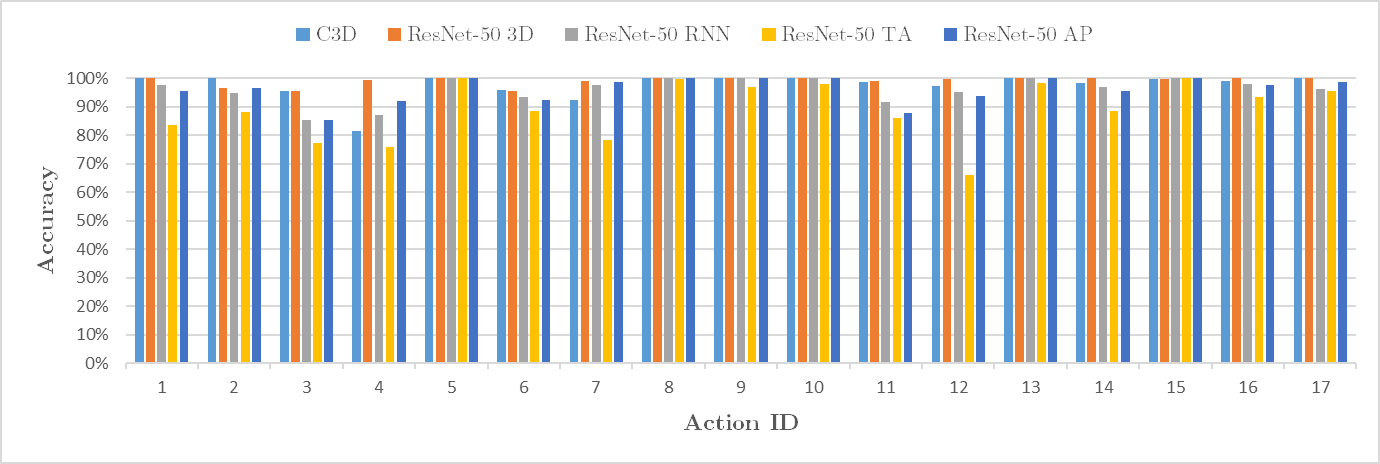
\includegraphics[width=1.0\linewidth]{Figs/pc-MvDA_confusion_muhavi.png}
        \caption{Comparison of accuracy on each action class using different deep features combined with pc-MvDA.}
        %\vspace{-0.3cm}
        \label{fig:pc-MvDA_confusion_muhavi}
    \end{figure}

    Table.\ref{tab:sota_muhavi} compares the best investigated combination of ResNet-50 3D and pc-MvDA with state-of-the-art frameworks. The comparison is for reference only because of aforementioned difference in setup of number of views and cross validation scheme.

    \begin{table}[htbp]
    \centering
    \caption{Comparison of the proposed methods with SOTA methods on MuHAVi dataset according to the second evaluation protocol.}
    \resizebox{0.7\textwidth}{!}{
    \begin{tabular}{|c|c|c|}
    \hline
    Methods                                                   & Cross-view & Multi-view \\ \hline
    Wu et al. \cite{wu2012view}                               & N/A       & 94.5     \\ \hline
    Zheng et al. \cite{zheng2016cross}                        & 94.88     & 99.8     \\ \hline
    Liu et al. \cite{liu2018learning}                         & N/A       & 91.2     \\ \hline
    Liu et al. \cite{liu2018hierarchically}                   & 99.91     & 99.8     \\ \hline
    Proposed method (ResNet-50 3D + pc-MvDA) \protect\footnotemark              & 99.90     & 99.88    \\ \hline
    \end{tabular}}
    \label{tab:sota_muhavi}
    \end{table}
    \footnotetext{Results when choosing only 4 views Camera 1, Camera 3, Camera 4 and Camera 6 following the other works.}

    %!TEX root = ../../../main.tex

\subsection{Experimental results on MICAGes dataset}

    \paragraph{1) Cross-view validation:} It can be seen in Table.\ref{tab:mica_cross} that pc-MvDA outperforms in almost every cases. With the first protocol, the norm accuracy of pc-MvDA of 74.52\% surpasses that of MvDA-vc (72.12\%) by 2.4\% and that of MvDA (64.94\%) by a large margin of 9.58\%. Especially in case of C3D features, the proposed algorithm achieved 90.2\% recognition rate whereas MvDA returns only 67.13\%.

    \begin{table}[htbp]
    \centering
    \caption{Cross-view recognition comparison on MICAGes dataset.}
    \resizebox{0.8\textwidth}{!}{
    \begin{tabular}{|c|c|c|c|c|c|c|}
        \hline
        \multirow{2}{*}{Deep features}          & \multicolumn{3}{c|}{Protocol 1}          & \multicolumn{3}{c|}{Protocol 2}            \\ \cline{2-7} 
                                                & MvDA  & MvDA-vc        & pc-MvDA         & MvDA  & MvDA-vc        & pc-MvDA           \\ \hline
        \multicolumn{1}{|c|}{C3D}               & 67.13 & 85.98          & \textbf{90.20}  & 93.74 & 99.80          & \textbf{100}      \\ \hline
        \multicolumn{1}{|c|}{ResNet-50 3D}      & 94.91 & 95.25          & \textbf{95.62}  & 97.43 & \textbf{99.97} & 99.79             \\ \hline
        \multicolumn{1}{|c|}{ResNet-50 RNN}     & 58.01 & 61.64          & \textbf{64.13}  & 100   & 100            & 100               \\ \hline
        \multicolumn{1}{|c|}{ResNet-50 TA}      & 53.58 & \textbf{59.55} & 58.62           & 96.70 & 99.48          & \textbf{99.83}    \\ \hline
        \multicolumn{1}{|c|}{ResNet-50 AP}      & 51.07 & 58.19          & \textbf{64.04}  & 99.73 & \textbf{99.99} & 99.89             \\ \hline
    \end{tabular}}
    \label{tab:mica_cross}
    \end{table}

    %Table.\ref{tab:cross_feature_mica} compares all types of deep features regarding accuracy of the proposed algorithm. 
    The top ranking of features applies identically and radically proves the superiority of 3D convolution based clip-level feature extraction in video recognition: ResNet-50 3D at 95.62\% and C3D at 90.2\%. The rest are ResNet-50 RNN (64.13\%), ResNet-50 AP (64.04\%) and ResNet-50 TA (58.62\%). For the second protocol, MvDA-vc (99.85\%) and pc-MvDA (99.9\%) are nearly even in performance while MvDA achieved 97.52\%.

    \begin{table}[htbp]
    \centering
    \caption{Cross-view recognition results of different features on MICAGes dataset with pc-MvDA method. The result in the bracket are accuracies of using features C3D, ResNet-50 3D, ResNet-50 RNN, ResNet-50 TA, RestNet-50 AP respectively. Each row corresponds to training view (from view K1 to view K5). Each column corresponds to testing view (from view K1 to view K5).}
    \resizebox{\textwidth}{!}{\begin{tabular}{|c|c|c|c|c|c|}
        \hline
        \backslashbox{Training}{Testing} & K1 & K2 & K3 & K4 & K5 \\ \hline
        K1 & N/A & \begin{tabular}{@{}c@{}} (92.9, \textbf{95.5}, 69.4, \\ 63.9, 65.1) \end{tabular} & \begin{tabular}{@{}c@{}} (93.7, \textbf{98.0}, 79.1, \\ 75.8, 74.7) \end{tabular} & \begin{tabular}{@{}c@{}} (90.5, \textbf{97.6}, 64.5, \\ 68.8, 70.8) \end{tabular} & \begin{tabular}{@{}c@{}} (89.2, \textbf{92.6}, 56.0, \\ 43.7, 58.2) \end{tabular} \\ \hline       
        K2 & \begin{tabular}{@{}c@{}} (84.7, \textbf{94.6}, 51.3, \\ 41.4, 53.7) \end{tabular} & N/A & \begin{tabular}{@{}c@{}} (94.6, \textbf{97.6}, 78.9, \\ 75.4, 77.5) \end{tabular} & \begin{tabular}{@{}c@{}} (91.3, \textbf{97.6}, 64.4, \\ 68.5, 68.0) \end{tabular} & \begin{tabular}{@{}c@{}} (87.4, \textbf{92.7}, 56.1, \\ 42.0, 55.6) \end{tabular} \\ \hline       
        K3 & \begin{tabular}{@{}c@{}} (87.5, \textbf{94.9}, 51.9, \\ 43.6, 52.7) \end{tabular} & \begin{tabular}{@{}c@{}} (93.0, \textbf{95.5}, 70.1, \\ 64.7, 63.4) \end{tabular} & N/A & \begin{tabular}{@{}c@{}} (90.0, \textbf{97.6}, 63.2, \\ 62.6, 67.5) \end{tabular} & \begin{tabular}{@{}c@{}} (88.9, \textbf{92.2}, 57.2, \\ 41.8, 56.6) \end{tabular} \\ \hline       
        K4 & \begin{tabular}{@{}c@{}} (86.7, \textbf{94.7}, 50.8, \\ 48.9, 54.9) \end{tabular} & \begin{tabular}{@{}c@{}} (90.2, \textbf{95.5}, 71.5, \\ 68.2, 61.8) \end{tabular} & \begin{tabular}{@{}c@{}} (92.5, \textbf{98.0}, 81.0, \\ 76.0, 74.4) \end{tabular} & N/A & \begin{tabular}{@{}c@{}} (89.7, \textbf{92.3}, 54.3, \\ 44.9, 56.6) \end{tabular} \\ \hline       
        K5 & \begin{tabular}{@{}c@{}} (84.9, \textbf{94.9}, 48.4, \\ 41.5, 57.9) \end{tabular} & \begin{tabular}{@{}c@{}} (90.4, \textbf{95.5}, 72.6, \\ 64.1, 65.7) \end{tabular} & \begin{tabular}{@{}c@{}} (94.0, \textbf{97.8}, 79.1, \\ 72.5, 76.3) \end{tabular} & \begin{tabular}{@{}c@{}} (91.9, \textbf{97.3}, 62.7, \\ 64.1, 69.0) \end{tabular} & N/A \\ \hline
    \end{tabular}}
    \label{tab:cross_feature_mica}
    \end{table}

    \paragraph{2) Multi-view validation}: The multi-view recognition results in Table.\ref{tab:mica_multi} shows an almost alike trend for both protocols. In general, pc-MvDA is 8.95\% and 0.72\% higher in accuracy for protocol 1, and 2.75\% and 0.04\% for protocol 2, in comparison with MvDA and MvDA-pc respectively.

    % TODO
    In virtually every experiments of MICAGes and two earlier benchmark datasets, the proposed extension is superior. The average accuracies of pc-MvDA is, in comparison on protocol 1 (and protocol 2 resp.), 5.29\% (1.21\% resp.) higher than MvDA, 1.21\% (0.62\% resp.) better than MvDA-vc. Despite not being as intuitive and straightly intelligible as pairwise-covariance, the multi-view resemblance added in MvDA-vc achieved nearly the performance of pc-MvDA. However, this view-consistency can be easily splitted into pairwise terms and intergrated into the objective of pc-MvDA in future works for further analysis.

    \begin{table}[htbp]
    \centering
    \caption{Multi-view recognition comparison on MICAGes dataset.}
    \resizebox{0.8\textwidth}{!}{
    \begin{tabular}{|c|c|c|c|c|c|c|}
        \hline
        \multirow{2}{*}{Deep features}          & \multicolumn{3}{c|}{Protocol 1}          & \multicolumn{3}{c|}{Protocol2}                     \\ \cline{2-7} 
                                                & MvDA  & MvDA-vc        & pc-MvDA         & MvDA           & MvDA-vc       & pc-MvDA           \\ \hline
        \multicolumn{1}{|c|}{C3D}               & 68.31 & 87.70          & \textbf{89.99}  & 88.79          & 99.54         & \textbf{100}      \\ \hline
        \multicolumn{1}{|c|}{ResNet-50 3D}      & 95.32 & 95.26          & \textbf{95.54}  & \textbf{100}   & 99.96         & 99.80             \\ \hline
        \multicolumn{1}{|c|}{ResNet-50 RNN}     & 57.50 & 63.05          & \textbf{63.83}  & 99.90          & \textbf{100}  & 99.97             \\ \hline
        \multicolumn{1}{|c|}{ResNet-50 TA}      & 54.43 & \textbf{61.46} & 58.25           & 96.72          & 99.49         & \textbf{99.69}    \\ \hline
        \multicolumn{1}{|c|}{ResNet-50 AP}      & 50.93 & 60.20          & \textbf{63.66}  & \textbf{99.99} & 99.93         & 99.67             \\ \hline
    \end{tabular}}
    \label{tab:mica_multi}
    \end{table}

    In addition to the same propensity shown, MICAGes also reveals the robustness of 3D convolution to generate fine clustered private feature space because this dataset contains exclusively hand gestures, which take part in a relatively small region of the captured videos. ResNet-50 3D and C3D are predominant for discriminant common space construction and classification and distances other features (Figure \ref{fig:pc-MvDA_confusion_mica}).

    \begin{figure}[htbp]
        \centering
        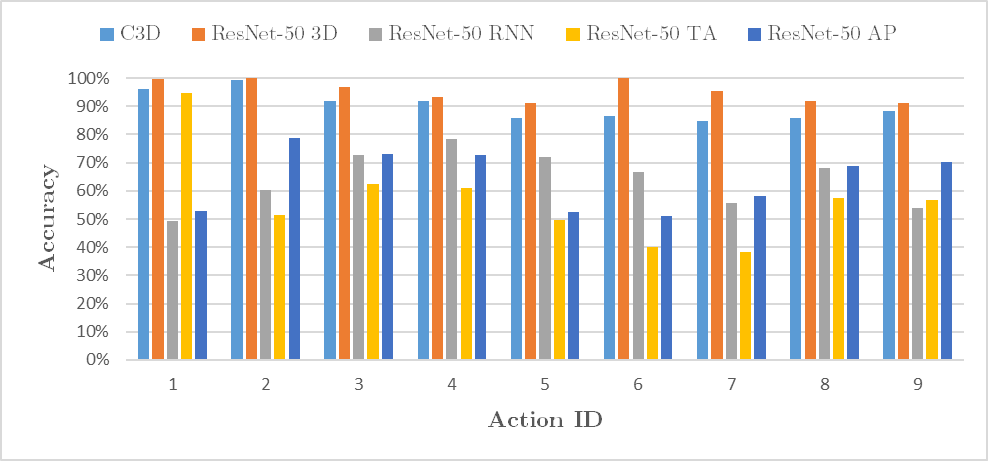
\includegraphics[width=0.8\linewidth]{figs/pc-MvDA_confusion_mica.png}
        \caption{Comparison of accuracy on each action class using different deep features combined with pc-MvDA on MICAGes dataset.}
        %\vspace{-0.3cm}
        \label{fig:pc-MvDA_confusion_mica}
    \end{figure}

    To better study the behavior of investigated multi-view analysis algorithms, t-SNE embedding of original private spaces, MvDA and pc-MvDA common space generated by protocol 1 are plotted in Figure \ref{fig:mica-tsne}. In these scatter plots, colors denote action classes, shapes as different views and train/test data are distinguished by border type. They explicitly denotes the surpassing capability of the proposed algorithm in finding a common space with prominent extra-class discrepancy. The data samples involved in training process are generally clustered in compact and separated blobs while testing data samples dissolve nearby. The better convergence of pc-MvDA compared to the baseline is usually only visible for harder features, whereas with the inputs of ResNet-50 3D features, which are already highly discriminated in private spaces, the improvement of pc-MvDA is negligible. Note that these illustrations of t-SNE embedding do not strictly depict an identical distribution of data.

    \begin{figure}[htbp]
        \centering
        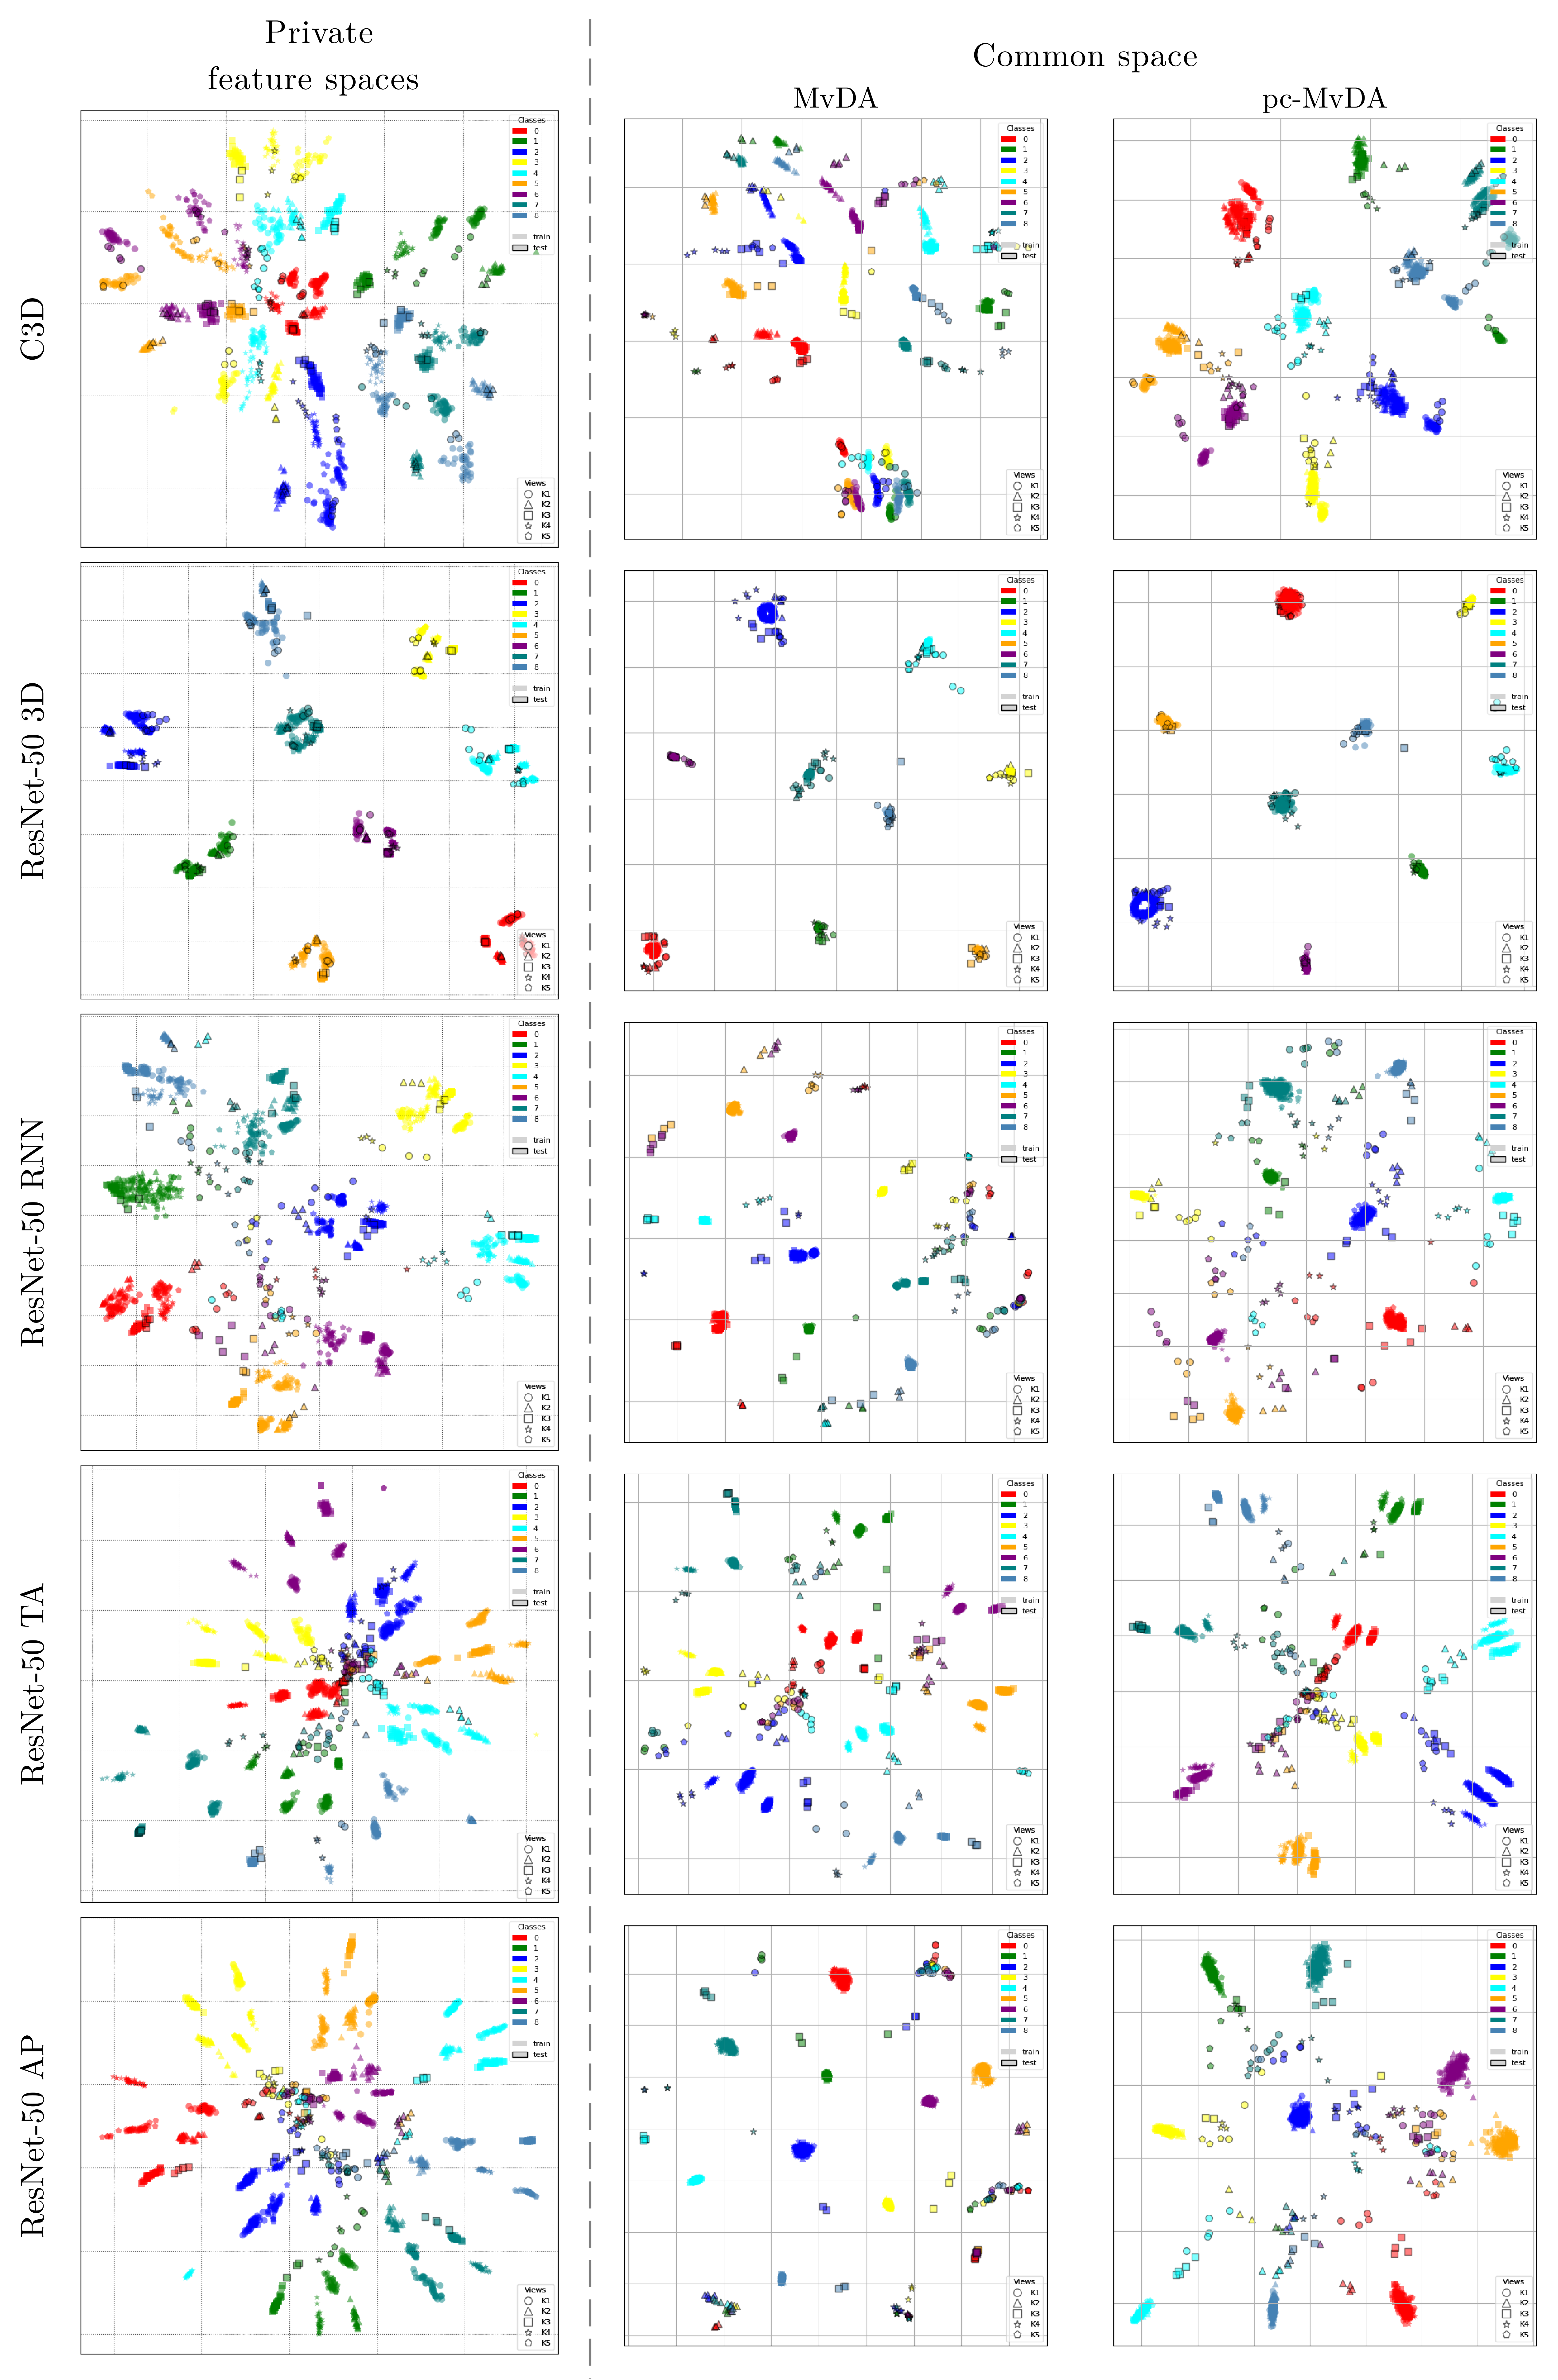
\includegraphics[width=1\linewidth, height=0.6\pdfpageheight, keepaspectratio=false]{figs/mica-tsne.png}
        \caption{First column: private feature spaces stacked and embedded together in a same coordinate system; Second column: MvDA common space; Third column: pc-MvDA common space.}
        %\vspace{-0.3cm}
        \label{fig:mica-tsne}
    \end{figure}



    \section{Summary}
        The experiments conducted indicates that the framework could achieve competitive results.
        The second evaluation protocol is shown to be less equitable for multi-view analysis algorithms compared to the first evaluation protocol represented in this thesis.
        Overall, the proposed pc-MvDA also achieved amelioration in almost every cases compared to baseline MvDA by a 5.29\% margin in terms of average accuracy.

    %!TEX root = ../../main.tex

\chapter{Conclusion} \label{chap:conclusion}
    %!TEX root = ../../main.tex

\section{Accomplishments}
    This thesis has presented a novel framework for human action recognition.
    The framework integrates various successful deep features with multi-view discriminant analysis to deal with cross-view human action recognition.
    In particular, five deep models have been utilized: ResNet with three pooling techniques; ResNet-3D and C3D.
    These deep features have been universally used for action recognition from a common view but rarely utilized for evaluating cross-view HAR.
    Besides, three variations of multi-view discriminant analysis: the original MvDA, MvDA with view consistency (MvDA-vc) and my proposed pairwise-covariance MvDA (pc-MvDA) have been investigated.
    Multi-view analysis algorithms have been successfully deployed for cross-view recognition of static images but never applied for spatio-temporal features.
    The experiments show that the proposed algorithm achieved highest average accuracy (5.29\% higher than MvDA and 1.21\% higher than MvDA-vc).
    % In addition, ResNet-50 3D gives the best overall HAR accuracy for both cross-view and multi-view evaluation protocols.
    % It concludes that the combination of deep features with pc-MvDA is suitable and feasible to deploy the proposed framework in practical applications. 

    %!TEX root = ../../main.tex

\section{Drawbacks} \label{sec:drawbacks}
    The overall framework is not end-to-end trainable.
    The proposed pc-MvDA is a batch algorithm, in effect, it is essential to process whole training dataset at once to compute class means at each optimization step.
    This makes pc-MvDA unsuitable to be a loss function that trains multiple large-scale neural networks concurrently, especially when input data is 3-dimensional spatio-temporal tensors.
    
    %!TEX root = ../../main.tex

\section{Future Works}


    %!TEX root = ../main.tex

\cleardoublepage
\ihead[]{Appendix}
\ohead[]{\pagemark}
\begin{appendix}
\chapter{Appendix}

\section{Derivation}\label{app:derivation}

We define the class vector $e_i \in \mathbb{R}^{\frac{n}{v}\times 1}$ which has $k^{th}$ element ${e_i}_{(k)} = 1$ if $class(x_k) = i$ and ${e_i}_{(k)} = 0$ otherwise.
It follows that $e = \sum_{i=1}^{c}e_i$ is a vector of ones.

\subsection{Derivation of \texorpdfstring{$\boldsymbol{S}^y_W$}{intra-class} and \texorpdfstring{$\boldsymbol{S}^y_B$}{inter-class} scatter matrices in MvDA} \label{subsec:derivation_mvda}

    \begin{equation}
        \begin{split}
            \boldsymbol{S}^y_W &= \sum_{i=1}^{c}\sum_{j=1}^{v}\sum_{k=1}^{n_{ij}}(y_{ijk}-\mu_i)(y_{ijk}-\mu_i)^T \\
            &= \sum_{i=1}^{c}\sum_{j=1}^{v}\sum_{k=1}^{n_{ij}}\left(y_{ijk}y_{ijk}^T - y_{ijk}\mu_i^T - \mu_iy_{ijk}^T + \mu_i\mu_i^T\right) \\
            &= \sum_{i=1}^{c}\left(\sum_{j=1}^{v}\sum_{k=1}^{n_{ij}}y_{ijk}y_{ijk}^T - n_i\mu_i\mu_i^T\right) \\
            &= \sum_{i=1}^{c}\left(\sum_{j=1}^{v}\sum_{k=1}^{n_{ij}}y_{ijk}y_{ijk}^T - \frac{1}{n_i}\left(\sum_{j=1}^{v}n_{ij}\mu_{ij}\right){\left(\sum_{j=1}^{v}n_{ij}\mu_{ij}\right)}^T\right) \\
            &= \sum_{i=1}^{c}\left(\sum_{j=1}^{v}\sum_{k=1}^{n_{ij}}y_{ijk}y_{ijk}^T - \frac{1}{n_i}\sum_{j=1}^{v}\sum_{r=1}^{v}n_{ij}n_{ir}\mu_{ij}\mu_{ir}^T\right) \\
            &= \sum_{j=1}^{v}\omega_j^T\left(\sum_{i=1}^{c}\sum_{k=1}^{n_{ij}}x_{ijk}x_{ijk}^T\right)\omega_j - \sum_{j=1}^{v}\sum_{r=1}^{v}\omega_j^T\left(\sum_{i=1}^{c}\frac{n_{ij}n_{ir}}{n_i}\mu^{(x)}_{ij}{\mu^{(x)}_{ir}}^T\right)\omega_r \\
            &= \sum_{j=1}^{v}\omega_j^T X_j I X_j^T\omega_j - \sum_{j=1}^{v}\sum_{r=1}^{v}\omega_j^T\left(\sum_{i=1}^{c}\frac{n_{ij}n_{ir}}{n_i}\left(\frac{1}{n_{ij}}X_j e_i\right)\left(\frac{1}{n_{ir}}X_r e_i\right)^T\right)\omega_r \\
            &= \sum_{j=1}^{v}\omega_j^T X_j I X_j^T\omega_j - \sum_{j=1}^{v}\sum_{r=1}^{v}\omega_j^T\left(\sum_{i=1}^{c}\frac{1}{n_i}X_j e_i e_i^T X_r^T\right)\omega_r \\
            &= \sum_{j=1}^{v}\omega_j^T X_j I X_j^T\omega_j - \sum_{j=1}^{v}\sum_{r=1}^{v}\omega_j^T X_j\left(\sum_{i=1}^{c}\frac{1}{n_i}e_i e_i^T\right)X_r^T\omega_r \\
            &= \sum_{j=1}^{v}\omega_j^T X_j I X_j^T\omega_j - \sum_{j=1}^{v}\sum_{r=1}^{v}\omega_j^T X_j E X_r^T\omega_r \\
            &= W^T X \boldsymbol{I} X^T W - W^T X \boldsymbol{E} X^T W \\
            &= W^T X \left(\boldsymbol{I} - \boldsymbol{E}\right) X^T W
        \end{split}
        \label{eq:mvda_Sw_derivation}
    \end{equation}
    where $I \in \mathbb{R}^{\frac{n}{v}\times \frac{n}{v}}$ and $\boldsymbol{I} \in \mathbb{R}^{n\times n}$ are identity matrices; $E = \sum_{i=1}^{c}\frac{1}{n_i}e_i e_i^T \in \mathbb{R}^{\frac{n}{v}\times \frac{n}{v}}$ is a square matrix whose elements satisfy:
    \begin{equation}
        \boldsymbol{E}_{(k,l)} = \left\{\begin{array}{lr}
            \frac{1}{n_i}, & \text{if } class(x_k) = class(x_l) = i\\
            0, & \text{otherwise}
            \end{array}\right\}
    \end{equation}
    and $\boldsymbol{E} = \left[E\right]_{v\times v} \in \mathbb{R}^{n\times n}$ is $v \times v$ grid stack of $E$:
    \begin{equation}
        \boldsymbol{E} = \left[\begin{matrix}E&E&\cdots&E\\E&E&\cdots&E\\\vdots&\vdots&\ddots&\vdots\\E&E&\cdots&E\\\end{matrix}\right]
    \end{equation}

    \begin{equation}
        \begin{split}
            \boldsymbol{S}^y_B &= \sum_{i=1}^{c}n_i\left(\mu_i - \mu\right)\left(\mu_i - \mu\right)^T \\
            &= \sum_{i=1}^{c}n_i\left(\mu_i\mu_i^T - \mu_i\mu^T - \mu\mu_i^T + \mu\mu^T\right) \\
            &= \sum_{i=1}^{c}n_i\mu_i\mu_i^T - n\mu\mu^T \\
            &= \sum_{i=1}^{c}n_i\left(\frac{1}{n_i}\sum_{j=1}^{v}n_{ij}\mu_{ij}\right)\left(\frac{1}{n_i}\sum_{j=1}^{v}n_{ij}\mu_{ij}\right)^T - n\left(\frac{1}{n}\sum_{i=1}^{c}\sum_{j=1}^{v}n_{ij}\mu_{ij}\right)\left(\frac{1}{n}\sum_{i=1}^{c}\sum_{j=1}^{v}n_{ij}\mu_{ij}\right)^T \\
            &= \sum_{i=1}^{c}\frac{1}{n_i}\left(\sum_{j=1}^{v}\sum_{r=1}^{v}n_{ij}n_{ir}\mu_{ij}\mu_{ir}^T\right) - \frac{1}{n}\left(\sum_{j=1}^{v}\sum_{i=1}^{c}n_{ij}\mu_{ij}\right)\left(\sum_{j=1}^{v}\sum_{i=1}^{c}n_{ij}\mu_{ij}\right)^T \\
            &= \sum_{j=1}^{v}\sum_{r=1}^{v}\left(\sum_{i=1}^{c}\frac{n_{ij}n_{ir}}{n_i}\mu_{ij}\mu_{ir}^T\right) - \frac{1}{n}\sum_{j=1}^{v}\sum_{r=1}^{v}\left(\sum_{i=1}^{c}n_{ij}\mu_{ij}\right)\left(\sum_{i=1}^{c}n_{ij}\mu_{ij}\right)^T \\
            &= \sum_{j=1}^{v}\sum_{r=1}^{v}\left(\sum_{i=1}^{c}\frac{n_{ij}n_{ir}}{n_i}\mu_{ij}\mu_{ir}^T\right) - \frac{1}{n}\sum_{j=1}^{v}\sum_{r=1}^{v}\left(\sum_{a=1}^{c}\sum_{b=1}^{c}n_{aj}n_{br}\mu_{aj}\mu_{br}^T\right) \\
            &= \sum_{j=1}^{v}\sum_{r=1}^{v}\omega_j^T\left(\sum_{i=1}^{c}\frac{n_{ij}n_{ir}}{n_i}\mu^{(x)}_{ij}{\mu^{(x)}_{ir}}^T\right)\omega_r - \sum_{j=1}^{v}\sum_{r=1}^{v}\omega_j^T\left(\sum_{a=1}^{c}\sum_{b=1}^{c}\frac{n_{aj}n_{br}}{n}\mu^{(x)}_{aj}{\mu^{(x)}_{br}}^T\right)\omega_r \\
            &= \sum_{j=1}^{v}\sum_{r=1}^{v}\omega_j^T\left(\sum_{i=1}^{c}\frac{n_{ij}n_{ir}}{n_i}\left(\frac{1}{n_{ij}}X_j e_i\right)\left(\frac{1}{n_{ir}}X_r e_i\right)^T\right)\omega_r \\
            &\ \ \ \ \ \ \ \ \ \ \ \ \ \ \ \ \ \ \ \ \ \ \ \ \ \ \ \ \ \  - \sum_{j=1}^{v}\sum_{r=1}^{v}\omega_j^T\left(\sum_{a=1}^{c}\sum_{b=1}^{c}\frac{n_{aj}n_{br}}{n}\left(\frac{1}{n_{aj}}X_j e_a\right)\left(\frac{1}{n_{br}}X_r e_b\right)\right)\omega_r \\
            &= \sum_{j=1}^{v}\sum_{r=1}^{v}\omega_j^T X_j\left(\sum_{i=1}^{c}\frac{1}{n_i}e_i e_i^T\right)X_r^T\omega_r - \sum_{j=1}^{v}\sum_{r=1}^{v}\omega_j^T X_j\left(\sum_{a=1}^{c}\sum_{b=1}^{c}\frac{1}{n}e_a e_b^T\right)X_r^T\omega_r \\
            &= \sum_{j=1}^{v}\sum_{r=1}^{v} \omega_j^T X_j E X_r^T \omega_r - \sum_{j=1}^{v}\sum_{r=1}^{v} \omega_j^T X_j \mathbbm{1} X_r^T \omega_r \\
            &= W^T X \boldsymbol{E} X^T W - W^T X \boldsymbol{\mathbbm{1}} X^T W \\
            &= W^T X \left(\boldsymbol{E} - \boldsymbol{\mathbbm{1}}\right) X^T W
        \end{split}
        \label{eq:mvda_Sb_derivation}
    \end{equation}
    where $E = \sum_{i=1}^{c}\frac{1}{n_i}e_i e_i^T \in \mathbb{R}^{\frac{n}{v}\times \frac{n}{v}}$ and $\boldsymbol{E} = \left[E\right]_{v\times v} \in \mathbb{R}^{n\times n}$ are defined above; $\mathbbm{1} = \sum_{a=1}^{c}\sum_{b=1}^{c}e_a e_b^T = \left[1\right]_{\frac{n}{v} \times \frac{n}{v}} \in \mathbb{R}^{\frac{n}{v}\times \frac{n}{v}}$ and $\boldsymbol{\mathbbm{1}} = \left[\mathbbm{1}\right]_{v\times v} = \left[1\right]_{n \times n} \in \mathbb{R}^{n\times n}$ are matrices of ones.

\subsection{Derivation of \texorpdfstring{$\boldsymbol{O}_{view-consistency}$}{view-consistency term} in MvDA-vc} \label{subsec:derivation_mvdavc}

    \begin{equation}
        \begin{split}
            \boldsymbol{O}_{view-consistency} &= \sum_{j=1}^{v}\sum_{r=1}^{v}\left|\left|\beta_j - \beta_r\right|\right|_2^2 \\
            &= \sum_{j=1}^{v}\sum_{r=1}^{v}\left(\beta_j^T\beta_j - \beta_j^T\beta_r - \beta_r^T\beta_j + \beta_r^T\beta_r\right) \\
            &= \sum_{j=1}^{v}\sum_{r=1}^{v}\left(2\beta_j^T\beta_j - 2\beta_j^T\beta_r\right) \\
            &= \sum_{j=1}^{v}2v\omega_j^T\boldsymbol{P}_j I \boldsymbol{P}_j^T\omega_j - \sum_{j=1}^{v}\sum_{r=1}^{v}2\omega_j^T\boldsymbol{P}_j I \boldsymbol{P}_r^T\omega_r \\
            &= W^T \boldsymbol{P}^T \left(2v\boldsymbol{I}\right) \boldsymbol{P} W - W^T \boldsymbol{P}^T \left(2\boldsymbol{\widehat{I}}\right) \boldsymbol{P} W \\
            &= W^T \boldsymbol{P}^T \left(2v\boldsymbol{I} - 2\boldsymbol{\widehat{I}}\right) \boldsymbol{P} W
        \end{split}
        \label{eq:mvdavc_vc_derivation}
    \end{equation}
    where $\beta_j = \boldsymbol{P}_j\omega_j$ and $\boldsymbol{P}_j = \left(X_j^T X_j\right)^{-1}X_j^T$ as defined in Section \ref{subsubsec:mvdavc}; $I \in \mathbb{R}^{\frac{n}{v}\times \frac{n}{v}}$ and $\boldsymbol{I} \in \mathbb{R}^{n\times n}$ are defined in \ref{subsec:derivation_mvda}, $\boldsymbol{\widehat{I}} = \left[I\right]_{v\times v} \in \mathbb{R}^{n\times n}$ is $v\times v$ grid stack of $I$:
    \begin{equation}
        \boldsymbol{\widehat{I}} = \left[\begin{matrix}I&I&\cdots&I\\I&I&\cdots&I\\\vdots&\vdots&\ddots&\vdots\\I&I&\cdots&I\\\end{matrix}\right]
    \end{equation}

\subsection{Derivation of \texorpdfstring{${\boldsymbol{S}^x_W}_{ab}$}{paired intra-class} and \texorpdfstring{${\boldsymbol{S}^x_B}_{ab}$}{paired inter-class} scatter matrices in pc-MvDA} \label{subsec:derivation_pcmvda}

    Firstly we reformulate the local intra-class ${\boldsymbol{S}^x_W}_{i}$ from Equation \eqref{eq:pcmvda_Sw_i}.
    It can be easily derived by removing sum over classes $\sum_{i=1}^{c}$ from $\boldsymbol{S}_W^y$ in Equation \eqref{eq:mvda_Sw_derivation}:
    \begin{equation}
        \begin{split}
            {\boldsymbol{S}_W^y}_i &= \sum_{j=1}^{v}\sum_{k=1}^{n_{ij}}\left(y_{ijk}-\mu_i\right)\left(y_{ijk}-\mu_i\right)^T \\
            &= \sum_{j=1}^{v}\omega_j^T\left(\sum_{k=1}^{n_ij}x_{ijk}x_{ijk}^T\right)\omega_j - \sum_{j=1}^{v}\sum_{r=1}^{v}\omega_j^T X_j\left(\frac{1}{n_i} e_i e_i^T\right)X_r^T\omega_r \\
            &= \sum_{j=1}^{v}\omega_j^T X_j I_i X_j^T\omega_j - \sum_{j=1}^{v}\sum_{r=1}^{v}\omega_j^T X_j E X_r^T\omega_r \\
            &= W^T X \boldsymbol{I}_i X^T W - W^T X \boldsymbol{E} X^T W \\
            &= W^T X \left(\boldsymbol{I}_i - \boldsymbol{E}\right) X^T W
        \end{split}
        \label{eq:pcmvda_Sw_i_derivation}
    \end{equation}
    where $E \in \mathbb{R}^{\frac{n}{v}\times \frac{n}{v}}$ and $\boldsymbol{E} \in \mathbb{R}^{n\times n}$ are defined in Section \ref{subsec:derivation_mvda}; $I_{i} = I e_i \in \mathbb{R}^{\frac{n}{v}\times \frac{n}{v}}$ is $e_i$ masked identity matrix whose elements satisfy:
    \begin{equation}
        {\boldsymbol{I}_{i}}_{(k,k)} = \left\{\begin{array}{lr}
            1, & \text{if } class(x_k) = i \\
            0, & \text{otherwise}
            \end{array}\right\}
    \end{equation}
    and $\boldsymbol{I}_{i} \in \mathbb{R}^{n\times n}$ is $v$ diagonal stack of $I_i$:
    \begin{equation}
        \boldsymbol{I}_{i} = \left[\begin{matrix}I_i&0&\cdots&0\\0&I_i&\cdots&0\\\vdots&\vdots&\ddots&\vdots\\0&0&\cdots&I_i\\\end{matrix}\right]
    \end{equation}

    Subtituing \eqref{eq:pcmvda_Sw_i_derivation} and \eqref{eq:mvda_Sw_derivation} in \eqref{eq:pcmvda_Sw_ab} we get:
    \begin{equation}
        \begin{split}
            {\boldsymbol{S}_W^y}_{ab} &= \beta\frac{n_a{\boldsymbol{S}_W^y}_a + n_b{\boldsymbol{S}_W^y}_b}{n_a + n_b} + (1 - \beta)\boldsymbol{S}_W^y \\
            &= \beta\frac{n_a W^T X \left(\boldsymbol{I}_a - \boldsymbol{E}\right) X^T W + n_b W^T X \left(\boldsymbol{I}_b - \boldsymbol{E}\right) X^T W}{n_a + n_b} + (1 - \beta)W^T X \left(\boldsymbol{I} - \boldsymbol{E}\right) X^T W \\
            &= W^T X \left(\beta\frac{n_a\left(\boldsymbol{I}_a - \boldsymbol{E}\right) + n_b\left(\boldsymbol{I}_b - \boldsymbol{E}\right)}{n_a + n_b} + (1 - \beta)\left(\boldsymbol{I} - \boldsymbol{E}\right)\right) X^T W \\
            &= W^T X \left(\beta\frac{n_a\boldsymbol{I}_a + n_b\boldsymbol{I}_b}{n_a + n_b} + (1 - \beta)\boldsymbol{I} - \boldsymbol{E}\right) X^T W
        \end{split}
        \label{eq:pcmvda_Sw_ab_derivation}
    \end{equation}
    where $0 \leq \beta \leq 1$ is a hyperparameter.

    \begin{equation}
        \begin{split}
            {\boldsymbol{S}_B^y}_{ab} &= {\left(\mu_a-\mu_b\right)\left(\mu_a-\mu_b\right)^T} \\
            &= \left[\sum_{j=1}^{v}\left(\frac{n_{aj}}{n_a}\mu_{aj} - \frac{n_{bj}}{n_b}\mu_{bj}\right)\right] \left[\sum_{j=1}^{v}\left(\frac{n_{aj}}{n_a}\mu_{aj} - \frac{n_{bj}}{n_b}\mu_{bj}\right)\right]^T \\
            &= \left[\sum_{j=1}^{v}\omega_j^T\left(\frac{n_{aj}}{n_a}\mu^{(x)}_{aj} - \frac{n_{bj}}{n_b}\mu^{(x)}_{bj}\right)\right] \left[\sum_{j=1}^{v}\omega_j^T\left(\frac{n_{aj}}{n_a}\mu^{(x)}_{aj} - \frac{n_{bj}}{n_b}\mu^{(x)}_{bj}\right)\right]^T \\
            &= \left[\sum_{j=1}^{v}\omega_j^T\left(\frac{n_{aj}}{n_a}\left(\frac{1}{n_{aj}}X_j e_a\right) - \frac{n_{bj}}{n_b}\left(\frac{1}{n_{bj}}X_j e_b\right)\right)\right] \\
            &\ \ \ \ \ \ \ \ \ \ \ \ \ \ \ \ \ \ \ \ \ \ \ \ \ \ \ \ \ \ \left[\sum_{j=1}^{v}\omega_j^T\left(\frac{n_{aj}}{n_a}\left(\frac{1}{n_{aj}}X_j e_a\right) - \frac{n_{bj}}{n_b}\left(\frac{1}{n_{bj}}X_j e_b\right)\right)\right]^T \\
            &= \left[\sum_{j=1}^{v}\omega_j^T X_j\left(\frac{1}{n_a}e_a - \frac{1}{n_b}e_b\right)\right] \left[\sum_{j=1}^{v}\omega_j^T X_j\left(\frac{1}{n_a}e_a - \frac{1}{n_b}e_b\right)\right]^T \\
            &= \sum_{j=1}^{v}\sum_{r=1}^{v}\omega_j^T X_j \left(\frac{1}{n_a}e_a - \frac{1}{n_b}e_b\right) \left(\frac{1}{n_a}e_a^T - \frac{1}{n_b}e_b^T\right) X_r^T\omega_r \\
            &= \sum_{j=1}^{v}\sum_{r=1}^{v}\omega_j^T X_j \left(\frac{1}{n_a^2}e_a e_a^T + \frac{1}{n_b^2}e_b e_b^T\right) X_r^T\omega_r - \sum_{j=1}^{v}\sum_{r=1}^{v}\omega_j^T X_j \frac{1}{n_a n_b}\left(e_a e_b^T + e_b e_a^T\right) X_r^T\omega_r \\
            &= \sum_{j=1}^{v}\sum_{r=1}^{v}\omega_j^T X_j E_{ab} X_r^T\omega_r - \sum_{j=1}^{v}\sum_{r=1}^{v}\omega_j^T X_j \tilde{E}_{ab} X_r^T\omega_r \\
            &= W^T X \boldsymbol{E}_{ab} X^T W - W^T X \boldsymbol{\tilde{E}}_{ab} X^T W \\
            &= W^T X \left(\boldsymbol{E}_{ab} - \boldsymbol{\tilde{E}}_{ab}\right) X^T W
        \end{split}
        \label{eq:pcmvda_Sb_i_derivation}
    \end{equation}
    where $E_{ab} = \frac{1}{n_a^2}e_a e_a^T + \frac{1}{n_b^2}e_b e_b^T \in \mathbb{R}^{\frac{n}{v}\times \frac{n}{v}}$ and $\tilde{E}_{ab} = \frac{1}{n_a n_b}\left(e_a e_b^T + e_b e_a^T\right) \in \mathbb{R}^{\frac{n}{v}\times \frac{n}{v}}$ are square matrices whose elements satisfy:
    \begin{align}
        {\boldsymbol{E}_{ab}}_{(k,l)} &= \left\{\begin{array}{lr}
            \frac{1}{{n_i}^2}, & \text{if } class(x_k) = class(x_l) = i \text{ and } i \in \{a, b\} \\
            0, & \text{otherwise}
            \end{array}\right\} \\
        {\boldsymbol{\tilde{E}}_{ab}}_{(k,l)} &= \left\{\begin{array}{lr}
            \frac{1}{n_a n_b}, & \text{if } i = class(x_k) \neq class(x_l) = j \text{ and } i,j \in \{a, b\} \\
            0, & \text{otherwise}
            \end{array}\right\}
    \end{align}
    and $\boldsymbol{E}_{ab} = \left[E_{ab}\right]_{v \times v} \in \mathbb{R}^{n\times n}$ and $\boldsymbol{\tilde{E}}_{ab} = \left[\tilde{E}_{ab}\right]_{v \times v} \in \mathbb{R}^{n\times n}$ are $v \times v$ grid stacks of $E_{ab}$ and $\tilde{E}_{ab}$ respectively:
    \begin{equation}
        \boldsymbol{E}_{ab} = \left[\begin{matrix}E_{ab}&E_{ab}&\cdots&E_{ab}\\E_{ab}&E_{ab}&\cdots&E_{ab}\\\vdots&\vdots&\ddots&\vdots\\E_{ab}&E_{ab}&\cdots&E_{ab}\\\end{matrix}\right]; \quad
        \boldsymbol{\tilde{E}}_{ab} = \left[\begin{matrix}\tilde{E}_{ab}&\tilde{E}_{ab}&\cdots&\tilde{E}_{ab}\\\tilde{E}_{ab}&\tilde{E}_{ab}&\cdots&\tilde{E}_{ab}\\\vdots&\vdots&\ddots&\vdots\\\tilde{E}_{ab}&\tilde{E}_{ab}&\cdots&\tilde{E}_{ab}\\\end{matrix}\right]
    \end{equation}

\normalsize
\end{appendix}


    \cleardoublepage
    \footnotesize
    \ihead[]{Bibliography}
    \bibliography{main}
    \normalsize

\end{document}
